\chapter{Análisis Sintáctico con {\tt Parse::Eyapp}}
\label{chapter:parseeyapp}
\section{Conceptos Básicos para el Análisis Sintáctico}
\label{section:conceptosbasicosanalisissintactico}
Suponemos que el lector de esta sección ha realizado con éxito
un curso en teoría de autómatas y lenguajes formales.
Las siguientes definiciones repasan los conceptos mas importantes.

\begin{definition}
Dado un conjunto $A$, se define $A^*$ el cierre de Kleene de $A$ como:
\begin{math}
A^* = \cup_{n=0}^{\infty} A^n
\end{math}

Se admite que $A^0 = \{ \epsilon \}$, donde $\epsilon$ denota la palabra vacía, esto es
la palabra que tiene longitud cero, formada por cero símbolos del conjunto base $A$.
\end{definition}

\begin{definition}
Una gramática $G$ es una cuaterna $G =(\Sigma,V,P,S)$. 
$\Sigma$ es el conjunto de terminales. $V$ es un conjunto (disjunto de $\Sigma$)
que se denomina conjunto de \emph{variables sintácticas} o \emph{categorías gramáticales},
P es un conjunto de pares de $V \times (V \cup \Sigma )^*$. En vez de escribir
un par usando la notación $(A, \alpha) \in P$ se escribe $A \rightarrow \alpha$.
Un elemento de $P$ se denomina producción. Por último, $S$ es un símbolo del conjunto
$V$ que se denomina símbolo de arranque.
\end{definition}

\begin{definition}
Dada una gramática $G=(\Sigma,V,P,S)$ y $\mu = \alpha A \beta \in (V \cup \Sigma)^*$
una frase formada por variables y terminales y $A \rightarrow \gamma$ una producción de 
$P$, decimos que  $\mu$ deriva en un paso en  $\alpha \gamma \beta$. Esto es, derivar 
una cadena $\alpha A \beta$ es sustituir 
una variable sintáctica $A$ de $V$ por la parte derecha $\gamma$ de una de sus reglas de producción.
Se dice que $\mu$ deriva en $n$ pasos en $\delta$ si deriva en $n-1$ pasos en una cadena
$\eta$ la cual deriva en un paso en $\delta$. 
Se escribe entonces que $\mu  \stackrel{n}{\Longrightarrow}  \delta$. 
Una cadena deriva en 0 pasos en si misma.
Se escribe entonces que $\mu  \stackrel{*}{\Longrightarrow}  \delta$. 
\end{definition}

\begin{definition}
\label{definition:lenguajegenerado}
Dada una gramática $G=(\Sigma,V,P,S)$ se denota por $L(G)$ o lenguaje
generado por $G$ al lenguaje:

\begin{center}
$L(G) = \{ x \in \Sigma^* : S \stackrel{*}{\Longrightarrow} x \}$
\end{center}

Esto es, el lenguaje generado por la gramática $G$ esta formado por las cadenas
de terminales que pueden ser derivados desde el símbolo de arranque.
\end{definition}

\begin{definition}
Una derivación que comienza en el símbolo de arranque y termina en una secuencia
formada por sólo terminales de $\Sigma$ se dice \emph{completa}.

Una derivación $\mu  \stackrel{*}{\Longrightarrow}  \delta$ 
en la cual en cada paso $\alpha A x$ la regla de producción aplicada $A \rightarrow \gamma$
se aplica en la variable sintáctica mas a la derecha se dice \emph{una derivación a derechas}

Una derivación $\mu  \stackrel{*}{\Longrightarrow}  \delta$ 
en la cual en cada paso $x A \alpha$ la regla de producción aplicada $A \rightarrow \gamma$
se aplica en la variable sintáctica mas a la izquierda se dice \emph{una derivación a izquierdas}
\end{definition}

\begin{definition}
Observe que una derivación puede ser representada como un árbol cuyos nodos
están etiquetados en $V \cup \Sigma$. La aplicación de la regla de 
producción $A \rightarrow \gamma$ se traduce en asignar como hijos del nodo etiquetado con $A$
a los nodos etiquetados con los símbolos $X_1 \ldots X_n$ que constituyen
la frase $\gamma = X_1 \ldots X_n$.  
Este árbol se llama \cei{árbol sintáctico concreto} asociado 
con la derivación.
\end{definition}

\begin{definition}
\label{definition:arbolconcreto}
Observe que, dada una frase $x \in L(G)$ una derivación desde el
símbolo de arranque da lugar a  un árbol. Ese árbol tiene como raíz el 
símbolo de arranque y como hojas los terminales 
$x_1 \ldots x_n$ que forman $x$. Dicho árbol se denomina \emph{árbol
de análisis sintáctico concreto} de $x$. Una derivación determina
una forma de recorrido del árbol de análisis sintáctico concreto.
\end{definition}

\begin{definition}
Una gramática $G$ se dice ambigua si existe alguna frase $x \in L(G)$
con al menos dos árboles sintácticos. 
Es claro que esta definición es equivalente a afirmar que existe 
alguna frase $x \in L(G)$ para la cual existen dos derivaciones a 
izquierda (derecha) distintas.
\end{definition}

\begin{definition}
Un \cei{esquema de traducción} es una gramática independiente del contexto
en la cual se han insertado fragmentos de código en las partes derechas
de sus reglas de producción. 

\begin{center}
$A \rightarrow \alpha \{ action \}$
\end{center}

Los fragmentos de código asi insertados
se denominan \cei{acciones semánticas}. 


En un esquema de traducción los nodos del árbol sintáctico tienen asociados
\emph{atributos}. Si pensamos que cada nodo del árbol es un objeto, entonces
los atributos del nodo son los atributos del objeto. Las reglas semánticas
determinan la forma en la que son evaluados los atributos.

Los fragmentos de código de un esquema de traducción calculan
y modifican los atributos asociados con los nodos del árbol sintáctico.
El orden en que se evalúan los fragmentos
es el de \underline{un recorrido primero-profundo} del árbol de análisis sintáctico.
Esto significa que si en la regla 
$A \rightarrow \alpha \beta $
insertamos un fragmento de código:

\begin{center}
$A \rightarrow \alpha \{ action \} \beta $
\end{center}

La acción $\{ action \}$ se ejecutará después de todas las acciones
asociadas con el recorrido del subárbol de $\alpha$ y antes que todas
las acciones asociadas con el recorrido del subárbol $\beta$.

Obsérvese que para poder aplicar un esquema de traducción hay
que - al menos conceptualmente - construir el árbol sintáctico y 
después aplicar las acciones empotradas
en las reglas en el orden de recorrido primero-profundo. Por supuesto, \emph{si
la gramática es ambigua una frase podría tener dos árboles y la ejecución de las
acciones para ellos podría dar lugar a diferentes resultados}. Si se quiere
evitar la multiplicidad de resultados (interpretaciones semánticas)
es necesario precisar de que árbol sintáctico concreto se esta hablando.

\end{definition}

\begin{definition}
Un atributo tal que su valor en un nodo
puede ser computado en términos de los atributos de los hijos del nodo se dice
que es un \cei{atributo sintetizado}.
\end{definition}

El siguiente esquema de traducción recibe como entrada una expresión en infijo
y produce como salida su traducción a postfijo para expresiones aritmeticas con sólo 
restas de números:

\vspace{0.5cm}
\begin{tabular}{ll}
$expr   \rightarrow expr_1  -  NUM$  & \verb|{ $expr{TRA} = $expr[1]{TRA}." ".$NUM{VAL}." - "}| \\
$expr   \rightarrow NUM$             & \verb|{ $expr{TRA} = $NUM{VAL} }|
\end{tabular}
\vspace{0.5cm}

Que para una entrada \verb|2 - 3 - 7| daría lugar a la siguiente evaluación:

\begin{verbatim}
e '2 3 - 7 -'
`-- --- e '2 3 -'
    |   `------ e '2'
    |       |    `-- N 2
    |       |-- '-'
    |       `-- N 3
    |-- '-'
    `-- N 7
\end{verbatim}


\begin{definition}
Un \cei{atributo heredado} es aquel cuyo valor se computa a partir de los
valores de sus hermanos y de su padre.
\end{definition}

\begin{example}
\label{example:eyapptypesandts}
Un ejemplo de atributo heredado es el tipo de las variables en las declaraciones:

\vspace{0.5cm}
\begin{tabular}{ll}
$decl   \rightarrow type$ \verb|{ $list{T} = $type{T} }| $list$\\
$type   \rightarrow INT$ \verb|{ $type{T} = $int }|\\
$type   \rightarrow STRING$ \verb|{ $type{T} = $string }|\\
$list   \rightarrow ID$ , \verb|{ $ID{T} = $list{T}; $list_1{T} = $list{T} }| $list_1$\\
$list   \rightarrow ID$ \verb|{ $ID{T} = $list{T} }|
\end{tabular}
\vspace{0.5cm}
\end{example}


\section{{\tt Parse::Eyapp}: Un Generador de Analizadores Sintácticos}
\label{section:ungeneradordeanalizadoressintacticos}
El generador de analizadores sintácticos \tei{Parse::Eyapp} es un
analizador LALR inspirado en \tei{yacc}. 
\htmladdnormallink{Parse::Eyapp}{http://search.cpan.org/~casiano/Parse-Eyapp/}
es una extensión de 
\htmladdnormallink{Parse::Yapp}{http://search.cpan.org/~fdesarmenien/Parse-Yapp/}
escrita por Casiano
Rodriguez-Leon. Puede descargarlo desde CPAN e instalarlo en su máquina siguiendo
el procedimiento habitual.

El generador de analizadores sintácticos \tei{Parse::Eyapp} que
estudiaremos en las siguientes secciones funciona de manera similar
a un esquema de traducción. Las reglas de producción de la gramática
son aumentadas con reglas semánticas. Los símbolos que aparecen en la regla
de producción tienen \emph{atributos} asociados y las reglas semánticas
dicen como deben ser computados dichos atributos.
Consideremos, por ejemplo, el siguiente fragmento de programa \verb|eyapp|:

\begin{center}
\begin{tabular}{p{12cm}}
\begin{verbatim}
exp:  exp '+' exp         { $_[1] + $_[3] }
\end{verbatim}\\
\end{tabular}
\end{center}

que dice que asociado con el símbolo $exp$ de la regla de producción  $exp \rightarrow exp '+' exp$ 
tenemos el atributo  \underline{valor} numérico y que para computar el atributo 
\underline{valor} de la variable sintáctica $exp$ en la parte izquierda tenemos
que sumar los atributos asociados con los símbolos primero y tercero de la parte derecha.

Por defecto \verb|Parse::Eyapp| no provee un esquema de traducción ya que - aunque el orden de
ejecucíon de las acciones es de abajo-arriba y de izquierda a derecha como en un esquema -
no es posible acceder a atributos de nodos que aún no han sido visitados.

Para ilustrar el uso de \verb|Parse::Eyapp| veamos
un ejemplo en el que se implanta una gramática
cuyas frases son secuencias (separadas por retornos de carro)
de expresiones aritméticas.

Los contenidos del programa \tei{eyapp} los hemos guardado
en un fichero denominado \verb|CalcSyntax.eyp|

\parrafo{Partes de un Programa {\tt Eyapp}}

Un programa \verb|eyapp| consta de tres partes: 

\begin{itemize}
\item
la cabeza, 
\item
el cuerpo
\item
y la cola. 
\end{itemize}

Cada una de las partes va separada de las otras por el
símbolo \verb|%%| en una línea aparte. 

Así, el \verb|%%| de la línea 8
separa la cabeza del cuerpo y el de la línea 31 el cuerpo de la cola. 

\begin{itemize}
\item
En la cabecera se colocan el
código de inicialización, las declaraciones de terminales, las reglas
de precedencia, etc.  

\item
El cuerpo contiene las reglas de la gramática y
las acciones asociadas. 

\item
Por último, la cola de un program \verb|eyapp|
contiene las rutinas de soporte al código que aparece en las acciones 
asi como, posiblemente, rutinas para el análisis léxico 
y el tratamiento de errores.
\end{itemize}

\begin{verbatim}
pl@nereida:~/LEyapp/examples$ cat -n CalcSyntax.eyp
 1  # CalcSyntax.eyp
 2  %right  '='
 3  %left   '-' '+'
 4  %left   '*' '/'
 5  %left   NEG
 6  %right  '^'
 7
 8  %%
 9
10  input:  line *  { print "input -> line *\n" }
11  ;
12
13  line:
14    '\n'         { print "line -> \\n\n" }
15    | exp '\n'   { print "line -> exp \\n\n"}
16  ;
17
18  exp:
19      NUM                { print "exp -> NUM ($_[1])\n"; }
20    | VAR                { print "exp -> VAR ($_[1])\n"; }
21    | VAR '=' exp        { print "exp -> VAR '=' exp\n"; }
22    | exp '+' exp        { print "exp -> exp '+' exp\n"; }
..    . ....................................................
29  ;
30
31  %%
32
33  sub _Error {
..    ....................................
41  }
42
..  ......................................
44
45  sub _Lexer {
46      my($parser)=shift;
..      .................
58  }
59
60  sub Run {
61      my($self)=shift;
62
63      $input = shift;
64      return $self->YYParse( yylex => \&_Lexer, yyerror => \&_Error );
65  }
\end{verbatim}

\parrafo{Las Reglas}

Todas las partes derechas de las reglas de producción de una misma variable sintáctica se escriben
juntas separadas mediante la barra vertical \verb#|#.

\begin{verbatim}
10  input:  line *  { print "input -> line *\n" }
11  ;
12
13  line:
14    '\n'         { print "line -> \\n\n" }
15    | exp '\n'   { print "line -> exp \\n\n"}
16  ;
\end{verbatim}

En este ejemplo hemos simplificado las acciones semánticas 
reduciéndolas a mostrar la regla de producción encontrada.

\parrafo{Reglas de Producción Vacías}
\label{parrafo:reglasvacias}

Un asterisco (como en la línea 10) indica repetición cero o mas veces
de la expresión a la que se aplica.
De hecho la línea 10 es casi equivalente a:

\begin{verbatim}
input:  temp   
;
temp: 
    /* vacio */
  | temp line
;
\end{verbatim}

Observe como en el código anterior
hemos codificado la regla de producción $temp \rightarrow \epsilon$
como:

\begin{verbatim}
temp: 
    /* vacio */
\end{verbatim}

Es buena costumbre de programación
cuando se tiene una regla de producción que produce vacío 
ponerla la primera del grupo y añadir un comentario como este.
Dado que vacío se representa en \verb|Eyapp| mediante la cadena vacía
es fácil que pase desapercibida. Es por ello que se recomienda
que \emph{una regla vacía sea siempre la primera y que este comentada}
como en el ejemplo.


\parrafo{Tratamiento de las Ambiguedades}

Hay numerosas ambiguedades en esta gramática. 
Observe las reglas para los diferentes tipos de expresiones:

\begin{verbatim}
18 exp:
19     NUM                { print "exp -> NUM ($_[1])\n"; }
20   | VAR                { print "exp -> VAR ($_[1])\n"; }
21   | VAR '=' exp        { print "exp -> VAR '=' exp\n"; }
22   | exp '+' exp        { print "exp -> exp '+' exp\n"; }
23   | exp '-' exp        { print "exp -> exp '-' exp\n"; }
24   | exp '*' exp        { print "exp -> exp '*' exp\n"; }
25   | exp '/' exp        { print "exp -> exp '/' exp\n"; }
26   | '-' exp %prec NEG  { print "exp -> '-' exp\n"; }
27   | exp '^' exp        { print "exp -> exp '^' exp\n"; }
28   | '(' exp ')'        { print "exp -> '(' exp ')'\n"; }
29 ;
\end{verbatim}

Surgen preguntas como:

\begin{itemize}
\item
¿Como debo interpretar la expresión \verb|4 - 5 - 2|?
¿Como \verb|(4 - 5) - 2|? ¿o bien \verb|4 - (5 - 2)|?
La respuesta la da la asignación de asociatividad a los operadores
que hicimos en la cabecera:
\begin{verbatim}
1 # CalcSyntax.eyp
2 %right  '='
3 %left   '-' '+'
4 %left   '*' '/'
5 %left   NEG
6 %right  '^'
7
8 %%
\end{verbatim}

\parrafo{La Asociatividad de Terminales y la Ambiguedad}

Las declaraciones \tei{\%left} y \tei{\%right} expresan la asociatividad
y precedencia de los terminales, permitiendo decidir que árbol construir 
en caso de  ambiguedad. 

\emph{ Los terminales declarados en líneas 
posteriores tienen mas prioridad que los declarados en las líneas anteriores}.

Por defecto, \emph{una regla de producción
tiene la prioridad del último terminal que aparece
en su parte derecha}.

Al declarar como asociativo a izquierdas al terminal \verb|-| 
hemos 
resuelto la ambiguedad en \verb|4 -5 -2|. Lo que estamos haciendo es
indicarle al analizador que a la hora de elegir entre 
los árboles abstractos 
$-(-(4,5),2)$ y $-(4, -(5,2))$ elija siempre
el árbol que se hunde a izquierdas.
\item
¿Como debo interpretar la expresión \verb|4 - 5 * 2|?
¿Como \verb|(4 - 5) * 2|? ¿o bien \verb|4 - (5 * 2)|?
Al declarar que \verb|*| tiene mayor prioridad que \verb|-| estamos
resolviendo esta otra fuente de ambiguedad. Esto es así pues
\verb|*| fué declarado en la línea 11 y \verb|-| en la 10.
Por tanto el árbol será \verb|-(4, *(5,2))|.
\end{itemize}

La declaración de \verb|^| como asociativo a derechas y con un nivel
de prioridad alto resuelve las ambiguedades relacionadas 
con este operador:

\begin{verbatim}
  18  exp:
  ..    ......................................................
  28    | '(' exp ')'        { print "exp -> '(' exp ')'\n"; }

\end{verbatim}

\begin{exercise}
¿Como se esta interpretando la expresión \verb|-2^2|?
¿Cómo \verb|(-2)^2|? ¿o bien  \verb|-(2^2)|? 
\end{exercise}

\parrafo{Modificación de la Prioridad Implícita de una Regla}

Una regla de producción puede ir seguida de una directiva
\verb|%prec| la cual le da una prioridad explícita.  
Esto puede ser de gran ayuda en ciertos casos de 
ambiguedad.

\begin{verbatim}
26    | '-' exp %prec NEG  { print "exp -> '-' exp\n"; }
\end{verbatim}

¿Cual es la ambiguedad que surge con esta regla? 
La ambiguedad de esta regla 
esta relacionada con el doble significado
del menos como operador unario y binario: hay frases
como \verb|-y-z| que tiene dos posibles interpretaciones:
Podemos verla como \verb|(-y)-z| o bien como \verb|-(y-z)|.
Hay dos árboles posibles. El analizador, cuando este analizando
la entrada \verb|-y-z| y vea el
segundo \verb|-| (después de haber leído \verb|-y|)
deberá escoger uno de los dos árboles. 
¿Cuál?. El conflicto puede verse como una ``lucha'' entre
la regla \verb|exp: '-' exp| la cual interpreta la frase como
\verb|(-y)-z| y la segunda aparición del terminal \verb|-| 
el cuál ``quiere entrar'' para que gane la regla \verb|exp: exp '-' exp|
y dar lugar a la interpretación \verb|-(y-z)|.
En este caso, las dos reglas 
$E \rightarrow - E$ y $E \rightarrow E - E$ tienen, en principio
la prioridad del terminal \verb|-|, el cual fué declarado en la
zona de cabecera:
\begin{verbatim}
1 # CalcSyntax.eyp
2 %right  '='
3 %left   '-' '+'
4 %left   '*' '/'
5 %left   NEG
6 %right  '^'
7
8 %%
\end{verbatim}

La prioridad expresada explícitamente
para la regla por la declaración \verb|%prec NEG| de la línea
41 hace que la regla tenga la prioridad
del terminal \verb|NEG| y por tanto mas prioridad
que el terminal \verb|-|. Esto hará que \verb|eyapp| finalmente opte
por la regla \verb|exp: '-' exp| dando lugar a la interpretación
\verb|(-y)-z|.

\parrafo{La Cola}

Después de la parte de la gramática, y separada de la anterior
por el símbolo \verb|%%|, sigue la parte en la que se 
suelen poner las rutinas de apoyo. Hay al menos dos rutinas de apoyo que 
el analizador sintáctico requiere le sean pasados como argumentos: 
la de manejo de errores y la de análisis léxico. 

\begin{verbatim}
31  %%
32
33  sub _Error {
34          exists $_[0]->YYData->{ERRMSG}
35      and do {
36          print $_[0]->YYData->{ERRMSG};
37          delete $_[0]->YYData->{ERRMSG};
38          return;
39      };
40      print "Syntax error.\n";
41  }
42
43  my $input;
44
45  sub _Lexer {
46      my($parser)=shift;
47
48      # topicalize $input
49      for ($input) {
50        s/^[ \t]+//;      # skip whites
51        return('',undef) unless $input;
52
53        return('NUM',$1) if s{^([0-9]+(?:\.[0-9]+)?)}{};
54        return('VAR',$1) if s/^([A-Za-z][A-Za-z0-9_]*)//;
55        return($1,$1)    if s/^(.)//s;
56      }
57  }
58
59  sub Run {
60      my($self)=shift;
61
62      $input = shift;
63      return $self->YYParse( yylex => \&_Lexer, yyerror => \&_Error );
64  }
\end{verbatim}

\parrafo{El Método {\tt Run}}

El método \verb|Run|
ilustra como se hace la llamada al método de análisis sintáctico 
generado, utilizando la técnica de llamada con argumentos con nombre 
y pasándole las referencias a las dos subrutinas (en Perl,
es un convenio que si el nombre de una subrutina comienza
por un guión bajo es que el autor la considera privada):
\begin{verbatim}
78  sub Run {
79      my($self)=shift;
80
81      $input = shift;
82      return $self->YYParse( yylex => \&_Lexer, yyerror => \&_Error );
83  }
\end{verbatim}

\parrafo{El Atributo {\tt YYData} y el Método {\tt \_Error}}

El método \verb|YYData| provee acceso a un hash que contiene los datos 
que están siendo analizados. 

La subrutina de manejo de errores \verb|_Error| imprime 
el mensaje de error proveído por el usuario, el cual, si existe, fué guardado en
\verb|$_[0]->YYData->{ERRMSG}|.
\begin{verbatim}
51  sub _Error {
52          exists $_[0]->YYData->{ERRMSG}
53      and do {
54          print $_[0]->YYData->{ERRMSG};
55          delete $_[0]->YYData->{ERRMSG};
56          return;
57      };
58      print "Syntax error.\n";
\end{verbatim}

\parrafo{El Método {\tt \_Lexer}}
\label{parrafo:lexerparaeyapp}

A continuación sigue el método que implanta
el  análisis léxico \verb|_Lexer|.

\begin{verbatim}
45  sub _Lexer {
46      my($parser)=shift;
47
48      # topicalize $input
49      for ($input) {
50        s/^[ \t]+//;      # skip whites
51        return('',undef) unless $input;
52
53        return('NUM',$1) if s{^([0-9]+(?:\.[0-9]+)?)}{};
54        return('VAR',$1) if s/^([A-Za-z][A-Za-z0-9_]*)//;
55        return($1,$1)    if s/^(.)//s;
56      }
\end{verbatim}

El bucle \verb|for| constituye
en este caso una ''frase hecha'': el efecto es hacer que \verb|$_| sea un 
alias de \verb|$input|. Se simplifica la escritura (obsérvese que no es
necesario explicitar el operador de binding en las líneas 50-55,
no teniendo que escribir \verb|$input =~ s{^([0-9]+(?:\.[0-9]+)?)}{}|)
y que la computación será mas eficiente al acceder a través de \verb|$_| en vez de \verb|$input|.

El bucle \verb|for ($input)|
se ejecutará mientras la cadena
en \verb|$input| no sea vacía, lo que ocurrirá cuando todos 
los terminales hayan sido consumidos. sin embargo es un ''falso for'':
no hay iteración. El interior del bucle es ejecutado una sola vez en cada
llamada.

Eliminamos los blancos iniciales (lo que en inglés se conoce por
\cei{trimming}) y a
continuación vamos detectando los números, identificadores
y los símbolos individuales. 

En primer lugar se comprueba la existencia de
datos. Si no es el caso, estamos ante el
final de la entrada.
Cuando el analizador léxico alcanza el final de la entrada
debe devolver la pareja \verb|('',undef)|.

\begin{exercise}
\begin{enumerate}
\item ¿Quién es la variable índice en la línea 49? 
\item ¿Sobre quién ocurre el binding en las líneas 50-54? 
\item ¿Cual es la razón por la que \verb|$input| se 
ve modificado aún cuando no aparece como variable para el binding en las líneas 50-54?
\item Dada la entrada '\verb|4 * 3  |' con blancos al final:
como termina el analizador léxico. ¿Funciona correctamente en ese caso?
\end{enumerate}
\end{exercise}

\parrafo{Compilación con {\tt eyapp}}

Construimos el módulo \verb|CalcSyntax.pm| a partir del fichero \verb|CalcSyntax.eyp|
especificando la gramática, usando elejecutable \verb|eyapp|:
\begin{verbatim}
pl@nereida:~/LEyapp/examples$ eyapp -m CalcSyntax CalcSyntax.eyp
pl@nereida:~/LEyapp/examples$ ls -ltr | tail -3
-rw-r--r-- 1 pl users   1545 2007-10-24 09:03 CalcSyntax.eyp
-rwxr-xr-x 1 pl users    329 2007-10-24 09:05 usecalcsyntax.pl
-rw-r--r-- 1 pl users   7848 2007-10-24 09:36 CalcSyntax.pm
\end{verbatim}
Esta compilación genera el fichero \verb|CalcSyntax.pm| conteniendo el
analizador.

El script \verb|eyapp| es un \emph{frontend} al módulo \verb|Parse::Eyapp|.
Admite diversas formas de uso:

\begin{itemize}
\item
{\tt eyapp [options] \textit{grammar}[.eyp]}

Los sufijos {\tt .eyp} io {\tt .yp} son opcionales.
\item
{\tt eyapp \textit{-V}}

Nos muestra la versión:
\begin{verbatim}
pl@nereida:~/LEyapp/examples$ eyapp -V
This is Parse::Eyapp version 1.081.
\end{verbatim}

\item
{\tt eyapp \textit{-h}}

Nos muestra la ayuda:

\begin{verbatim}
pl@nereida:~/LEyapp/examples$ eyapp -h

Usage:  eyapp [options] grammar[.yp]
  or    eyapp -V
  or    eyapp -h

    -m module   Give your parser module the name <module>
                default is <grammar>
    -v          Create a file <grammar>.output describing your parser
    -s          Create a standalone module in which the driver is included
    -n          Disable source file line numbering embedded in your parser
    -o outfile  Create the file <outfile> for your parser module
                Default is <grammar>.pm or, if -m A::Module::Name is
                specified, Name.pm
    -t filename Uses the file <filename> as a template for creating the parser
                module file.  Default is to use internal template defined
                in Parse::Eyapp::Output
    -b shebang  Adds '#!<shebang>' as the very first line of the output file

    grammar     The grammar file. If no suffix is given, and the file
                does not exists, .yp is added

    -V          Display current version of Parse::Eyapp and gracefully exits
    -h          Display this help screen
\end{verbatim}

\end{itemize}

La opción \textit{-o outfile} \mbox{}
da el nombre del fichero de salida. Por defecto toma el nombre de la gramática,
seguido del sufijo \verb|.pm|. sin embargo, si hemos especificado la opción
\textit{-m A::Module::Name} el valor por defecto será  \emph{Name.pm}.

\parrafo{La Jerarquía de un Módulo y La Opción \textit{-m module}}

La opción \textit{-m module} \mbox{}
da el nombre  al paquete o espacio de nombres o clase encapsulando el
analizador. Por defecto toma el nombre de la gramática.  En el ejemplo anterior
podría haberse omitido. Sin embargo es necesaria cuando se esta desarrollando 
un módulo con un nombre complejo. Construyamos una distribución con
\verb|h2xs|:

\begin{verbatim}
$ h2xs -XA -n Calc::Syntax
Writing Calc-Syntax/lib/Calc/Syntax.pm
Writing Calc-Syntax/Makefile.PL
Writing Calc-Syntax/README
Writing Calc-Syntax/t/Calc-Syntax.t
Writing Calc-Syntax/Changes
Writing Calc-Syntax/MANIFEST
\end{verbatim}
Ahora añadimos el fichero \verb|.eyp| en el directorio de
la librería y producimos el módulo \verb|Syntax.pm|
al compilarlo. Para darle al paquete el nombre
\verb|Calc::Syntax| usamos la opción \verb|-m|:
\begin{verbatim}
$ cd Calc-Syntax/lib/Calc/
$ cp ~/LEyapp/examples/CalcSyntax.eyp .
$ eyapp -m Calc::Syntax  CalcSyntax.eyp
$  head -12 Syntax.pm | cat -n
     1  ###################################################################################
     2  #
     3  #    This file was generated using Parse::Eyapp version 1.081.
     4  #
     5  # (c) Parse::Yapp Copyright 1998-2001 Francois Desarmenien.
     6  # (c) Parse::Eyapp Copyright 2006 Casiano Rodriguez-Leon. Universidad de La Laguna.
     7  #        Don't edit this file, use source file "CalcSyntax.eyp" instead.
     8  #
     9  #             ANY CHANGE MADE HERE WILL BE LOST !
    10  #
    11  ###################################################################################
    12  package Calc::Syntax;
\end{verbatim}
La opción que recomiendo para documentar el módulo  es escribir
la documentación en un fichero aparte
\verb|Calc/Syntax.pod|.

\parrafo{El Programa Cliente}

A continuación escribimos el programa cliente:
\begin{verbatim}
$ cd ../..
$ mkdir scripts
$ cd scripts/
$ vi usecalcsyntax.pl
$ cat -n usecalcsyntax.pl
 1  #!/usr/bin/perl -w -I../lib
 2  use strict;
 3  use Calc::Syntax;
 4  use Carp;
 5
 6  sub slurp_file {
 7    my $fn = shift;
 8    my $f;
 9
10    local $/ = undef;
11    if (defined($fn)) {
12      open $f, $fn
13    }
14    else {
15      $f = \*STDIN;
16    }
17    my $input = <$f>;
18    return $input;
19  }
20
21  my $parser = Calc::Syntax->new();
22
23  my $input = slurp_file( shift() );
24  $parser->Run($input);
\end{verbatim}

\parrafo{Ejecución}

La ejecución muestra la \emph{antiderivación a derechas construida por {\tt eyapp}}:
\begin{verbatim}
$ cat prueba.exp
a=2*3

$ usecalcsyntax.pl prueba.exp
exp -> NUM (2)
exp -> NUM (3)
exp -> exp '*' exp
exp -> VAR '=' exp
line -> exp \n
input -> line *
\end{verbatim}


\parrafo{Orden de Ejecución de las Acciones Semánticas}

¿En que orden ejecuta \verb|YYParse| las acciones? 
La respuesta es que el analizador generado por 
\verb|eyapp| construye una derivación a derechas 
inversa y ejecuta las acciones asociadas a las reglas de producción
que se han aplicado. Así, para la frase \verb|2*3| la antiderivación es:

\begin{center}
\begin{math}
NUM + NUM \stackrel{NUM \leftarrow E}{\Longleftarrow} E + NUM \stackrel{NUM \leftarrow E}{\Longleftarrow} E + E \stackrel{E +E \leftarrow E}{\Longleftarrow} E
\end{math}
\end{center}

por tanto las acciones ejecutadas son las asociadas con las correspondientes reglas 
de producción:
\begin{enumerate}
\item
La acción asociada con $E \rightarrow NUM$:
\begin{verbatim}
 NUM                { print "exp -> NUM ($_[1])\n"; }
\end{verbatim}
Esta instancia de \verb|exp| tiene ahora como atributo \verb|2| (pasado por el analizador léxico).
\item
De nuevo la acción asociada con $E \rightarrow NUM$:
\begin{verbatim}
 NUM                { print "exp -> NUM ($_[1])\n"; }
\end{verbatim}
Esta nueva instancia de \verb|exp| tiene como atributo \verb|3|.
\item
La acción asociada con $E \rightarrow E * E$:
\begin{verbatim}
  | exp '*' exp        { print "exp -> exp '*' exp\n"; }
\end{verbatim}
\end{enumerate}
Obsérvese que la antiderivación a derechas da lugar a un
recorrido ascendente y a izquierdas del árbol:

\begin{equation*}
E_3(E_1(NUM[2]), *, E_2(NUM[2]))
\end{equation*}

Los subíndices indican el orden de visita de las nodos/producciones.

\section{Depuración de Errores}

Las fuentes de error
cuando se programa con una herramienta como \verb|eyapp| 
son diversas. En esta sección trataremos tres tipos de error:

\begin{itemize}
\item
Conflictos en la gramática: la gramática es ambigua o 
quizá - posiblemente debido a que en \verb|eyapp| se usa un sólo símbolo
de predicción - no queda claro para el generador 
que analizador sintáctico producir
\item
Ya no tenemos conflictos pero el analizador sintáctico
generado no se comporta como esperabamos: no acepta frases correctas
o construye un árbol erróneo para las mismas
\item
Ya hemos resuelto los conflictos y además el análisis sintáctico
es correcto pero tenemos errores semánticos. Los errores se producen
durante la ejecución de las acciones semánticas
\end{itemize}

\parrafo{Resolución de Conflictos}

El siguiente programa \verb|eyapp| contiene 
algunos errores. El lenguaje generado 
esta constituido por listas de \verb|D|s (por
declaraciones)
seguidas de listas de \verb|S|s (por sentencias)
separadas por puntos y coma:

\begin{verbatim}
pl@nereida:~/LEyapp/examples$ cat -n Debug.eyp
 1  %token D S
 2
 3  %{
 4  our $VERSION = '0.01';
 5  %}
 6
 7  %%
 8  p:
 9                  ds ';' ss
10          |       ss
11  ;
12
13  ds:
14            D ';' ds
15          | D
16            {
17              print "Reducing by rule:\n";
18              print "\tds -> D\n";
19              $_[1];
20            }
21  ;
22
23  ss:
24            S ';' ss
25          | S
26  ;
27
28  %%
29
30  my $tokenline = 0;
31
32  sub _Error {
33          my $parser = shift;
34          my ($token) = $parser->YYCurval;
35          my ($what) = $token ? "input: '$token'" : "end of input";
36          die "Syntax error near $what line num $tokenline\n";
37  }
38
39  my $input;
40
41  sub _Lexer {
42
43          for ($input) {
44            s{^(\s)}{} and $tokenline += $1 =~ tr{\n}{};
45            return ('',undef) unless $_;
46            return ($1,$1) if s/^(.)//;
47          }
48          return ('',undef);
49  }
50
51  sub Run {
52          my ($self) = shift;
53
54          $input = shift;
55
56          return $self->YYParse( yylex => \&_Lexer, yyerror => \&_Error,
57                           yydebug => 0xF
58    );
59  }
\end{verbatim}

Al compilar este programa con \verb|eyapp| produce un mensaje de advertencia anunciándonos
la existencia de un conflicto.
\begin{verbatim}
pl@nereida:~/LEyapp/examples$ eyapp Debug.eyp
1 shift/reduce conflict (see .output file)
State 4: shifts:
  to state    8 with ';'
\end{verbatim}
La existencia de advertencias da lugar a la creación de
un fichero \verb|Debug.output| conteniendo información
sobre la gramática y el analizador construido.

Veamos los contenidos del fichero:

\begin{verbatim}
pl@nereida:~/LEyapp/examples$ cat -n Debug.output
   1  Warnings:
   2  ---------
   3  1 shift/reduce conflict (see .output file)
   4  State 4: shifts:
   5    to state    8 with ';'
   6
   7  Conflicts:
   8  ----------
   9  State 4 contains 1 shift/reduce conflict
  10
  11  Rules:
  12  ------
  13  0:      $start -> p $end
  14  1:      p -> ds ';' ss
  15  2:      p -> ss
  16  3:      ds -> D ';' ds
  17  4:      ds -> D
  18  5:      ss -> S ';' ss
  19  6:      ss -> S
  20
  21  States:
  22  -------
  23  State 0:
  24
  25          $start -> . p $end      (Rule 0)
  26
  27          D       shift, and go to state 4
  28          S       shift, and go to state 1
  29
  30          p       go to state 2
  31          ss      go to state 3
  32          ds      go to state 5
  33
  ..  .........................................
  55  State 4:
  56
  57          ds -> D . ';' ds        (Rule 3)
  58          ds -> D .       (Rule 4)
  59
  60          ';'     shift, and go to state 8
  61
  62          ';'     [reduce using rule 4 (ds)]
  63
  ..  .........................................
  84  State 8:
  85
  86          ds -> D ';' . ds        (Rule 3)
  87
  88          D       shift, and go to state 4
  89
  90          ds      go to state 11
  91
  ..  .........................................
 112  State 12:
 113
 114          p -> ds ';' ss .        (Rule 1)
 115
 116          $default        reduce using rule 1 (p)
 117
 118
 119  Summary:
 120  --------
 121  Number of rules         : 7
 122  Number of terminals     : 4
 123  Number of non-terminals : 4
 124  Number of states        : 13
\end{verbatim}

El problema según se nos anuncia ocurre en el estado 4.
Como veremos mas adelante el analizador sintáctico
generado por \verb|Parse::Eyapp| es un autómata finito.
Cada estado guarda información sobre las reglas 
que podrían aplicarse durante el análisis de la entrada.
Veamos en detalle la información asociada con el estado 4:

\begin{verbatim}
  55  State 4:
  56
  57          ds -> D . ';' ds        (Rule 3)
  58          ds -> D .       (Rule 4)
  59
  60          ';'     shift, and go to state 8
  61
  62          ';'     [reduce using rule 4 (ds)]
  63
\end{verbatim}

Un estado es un conjunto de reglas de producción 
con un marcador en su parte derecha.
La idea es que - si estamos en un estado dado -
esas reglas son potenciales candidatos para la construcción
del árbol sintáctico. Que lo sean o no dependerá de los
terminales que se vean a continuación.

El punto que aparece en la parte derecha de una regla
indica ''posición'' de lectura. Así el hecho de que
en el estado cuatro aparezcan los items:

\begin{verbatim}
  57          ds -> D . ';' ds        (Rule 3)
  58          ds -> D .       (Rule 4)
\end{verbatim}

Significa que si estamos en este estado es por que se leyó
una \verb|D| y se espera ver un punto y 
coma. 

El comentario de la línea 60 indica que si el siguiente terminal es \verb|;|
podríamos ir  al estado 8. Obsérvese que el estado 8 contiene un item 
de la forma \verb|ds -> D ';' . ds|. La marca recuerda ahora que se vió 
una \verb|D| y un punto y coma.
El comentario de la línea 62:

\begin{verbatim}
  62          ';'     [reduce using rule 4 (ds)]
\end{verbatim}
indica que \verb|Parse::Eyapp| considera factible otro árbol cuando el token
actual es punto y coma: 
Reducir por la regla \verb|ds -> D|.

Para ilustrar el problema consideremos las frases
\verb|D;S| y \verb|D;D;S|. 

Para ambas frases,
después de consumir la \verb|D| el
analizador irá al estado 4 y el terminal actual será punto y coma.
Para la primera frase \verb|D;S| la decisión correcta 
es utilizar (''reducir'' en la jerga) la regla 4 \verb|ds -> D|.

Para la segunda frase \verb|D;D;S| la decisión correcta
es conjeturar la regla 3 \verb|ds -> D . ';' ds|.
El analizador podría saber que regla es la correcta si consumiera 
el terminal que sigue al punto y coma: si es \verb|S| se trata 
de la regla 4 y si es \verb|D| de la regla 3. Los analizadores generados 
por Eyapp no ''miran'' mas allá del siguiente terminal y por tanto
no están en condiciones de decidir.
 
Cualquier solución  a este tipo de conflictos
implica una reformulación de la gramática
modificando prioridades o reorganizando las reglas.
Reescribiendo la regla para \verb|ds| recursiva por la derecha
desaparece el conflicto:
\begin{verbatim}
l@nereida:~/LEyapp/examples$ sed -ne '/^ds:/,/^;/p' Debug1.eyp | cat -n
 1  ds:
 2            ds ';' D
 3          | D
 4      {
 5        print "Reducing by rule:\n";
 6        print "\tds -> D\n";
 7        $_[1];
 8      }
 9  ;
\end{verbatim}

Ahora ante una frase de la forma \verb|D ; ...| siempre hay que
reducir por \verb|ds -> D|. 
La antiderivación a derechas para \verb|D;D;S| es:

\begin{tabular}{|p{7cm}|p{5cm}|}
\hline
Derivación & Árbol\\
\hline
\begin{verbatim}
D;D;S <= ds;D;S <= ds;S <= ds;ss <= p
\end{verbatim}
&
p(ds(ds(D),';',D),';',ss(S))
\\
\hline
o\end{tabular}
Mientras que la antiderivación a derechas para \verb|D;S| es:

\begin{tabular}{|p{7cm}|p{5cm}|}
\hline
Derivación & Árbol\\
\hline
\begin{verbatim}
D;S <= ds;S <= ds;ss <= p
\end{verbatim}
&
p(ds(D),';',ss(S))
\\
\hline
\end{tabular}

Recompilamos la nueva versión de la gramática. 
Las advertencias han desaparecido:
\begin{verbatim}
pl@nereida:~/LEyapp/examples$ eyapp Debug1.eyp
pl@nereida:~/LEyapp/examples$ 
\end{verbatim}

\parrafo{Errores en la Construcción del Arbol}
\label{section:depuracion}

Escribimos el típico programa cliente:

\begin{verbatim}
pl@nereida:~/LEyapp/examples$ cat -n usedebug1.pl
 1  #!/usr/bin/perl -w
 2  # usetreebypass.pl prueba2.exp
 3  use strict;
 4  use Debug1;
 5
 6  sub slurp_file {
 7    my $fn = shift;
 8    my $f;
 9
10    local $/ = undef;
11    if (defined($fn)) {
12      open $f, $fn  or die "Can't find file $fn!\n";
13    }
14    else {
15      $f = \*STDIN;
16    }
17    my $input = <$f>;
18    return $input;
19  }
20
21  my $input = slurp_file( shift() );
22
23  my $parser = Debug1->new();
24
25  $parser->Run($input);
\end{verbatim}

y ejecutamos. 
Cuando damos la entrada \verb|D;S| introduciendo algunos blancos y retornos de carro
entre los terminales ocurre un mensaje de error:
\begin{verbatim}
casiano@cc111:~/LPLsrc/Eyapp/examples/debuggingtut$ usedebug1.pl
D

;

S
Reducing by rule:
        ds -> D
Syntax error near end of input line num 1
\end{verbatim}
Como esta  conducta es anómala activamos  la opción \verb|yydebug => 0xF| 
en la llamada a \verb|YYParser|.

Es posible añadir un parámetro en la llamada a \verb|YYParse|
con nombre \cei{yydebug} y valor el nivel de depuración requerido.
Ello 
nos permite observar la conducta del analizador. Los 
posibles valores de depuración son:

\vspace{0.5cm}
\begin{center}
\begin{tabular}{|l|l|}
\hline
   Bit      &    Información de Depuración \\
\hline
    0x01    &    Lectura de los terminales\\
\hline
    0x02    &    Información sobre los estados\\
\hline
    0x04    &    Acciones (shifts, reduces, accept \ldots)\\
\hline
    0x08    &    Volcado de la pila\\
\hline
    0x10    &    Recuperación de errores\\
\hline
\end{tabular}
\end{center}
\vspace{0.5cm}
 
Veamos que ocurre cuando damos la entrada \verb|D;S| introduciendo algunos blancos y retornos de carro
entre los terminales:
\begin{verbatim}
pl@nereida:~/LEyapp/examples$ usedebug1.pl
D

;

S

----------------------------------------
In state 0:
Stack:[0]
Need token. Got >D<
Shift and go to state 4.
----------------------------------------
In state 4:
Stack:[0,4]
Don't need token.
Reduce using rule 4 (ds --> D): Reducing by rule:
        ds -> D
Back to state 0, then go to state 5.
----------------------------------------
In state 5:
Stack:[0,5]
Need token. Got ><
Syntax error near end of input line num 1
\end{verbatim}
¿Que está pasando?
Vemos que después de leer \verb|D| el analizador sintáctico recibe 
un \verb|end of file|. Algo va mal en las comunicaciones entre el analizador léxico
y el sintáctico. Repasemos el analizador léxico:
\begin{verbatim}
pl@nereida:~/LEyapp/examples$ sed -ne '/sub.*_Lexer/,/^}/p' Debug1.eyp | cat -n
 1  sub _Lexer {
 2
 3          for ($input) {
 4             s{^(\s)}{} and $tokenline += $1 =~ tr{\n}{};
 5             return ('',undef) unless $_;
 6             return ($1,$1) if s/^(.)//;
 7          }
 8          return ('',undef);
 9  }
\end{verbatim}
El error está en la línea 4. ¡Sólo se consume un blanco!.
Escribimos una nueva versión \verb|Debug2.eyp| corrigiendo el 
problema:
\begin{verbatim}
pl@nereida:~/LEyapp/examples$ sed -ne '/sub.*_Lexer/,/^}/p' Debug2.eyp | cat -n
 1  sub _Lexer {
 2
 3          for ($input) {
 4             s{^(\s+)}{} and $tokenline += $1 =~ tr{\n}{};
 5             return ('',undef) unless $_;
 6             return ($1,$1) if s/^(.)//;
 7          }
 8          return ('',undef);
 9  }
\end{verbatim}

Ahora el análisis 
parece funcionar correctamente:
\begin{verbatim}
pl@nereida:~/LEyapp/examples$ usedebug2.pl
D

;

S

----------------------------------------
In state 0:
Stack:[0]
Need token. Got >D<
Shift and go to state 4.
----------------------------------------
In state 4:
Stack:[0,4]
Don't need token.
Reduce using rule 4 (ds --> D): Reducing by rule:
        ds -> D
Back to state 0, then go to state 5.
----------------------------------------
In state 5:
Stack:[0,5]
Need token. Got >;<
Shift and go to state 8.
----------------------------------------
In state 8:
Stack:[0,5,8]
Need token. Got >S<
Shift and go to state 1.
----------------------------------------
In state 1:
Stack:[0,5,8,1]
Need token. Got ><
Reduce using rule 6 (ss --> S): Back to state 8, then go to state 10.
----------------------------------------
In state 10:
Stack:[0,5,8,10]
Don't need token.
Reduce using rule 1 (p --> ds ; ss): Back to state 0, then go to state 2.
----------------------------------------
In state 2:
Stack:[0,2]
Shift and go to state 7.
----------------------------------------
In state 7:
Stack:[0,2,7]
Don't need token.
Accept.
\end{verbatim}

\parrafo{Errores en las Acciones Semánticas}

Un tercer tipo de error ocurre cuando el código 
de una acción semántica no se conduce como esperamos.

Las acciones semánticas son convertidas en métodos
anónimos del objeto analizador sintáctico
generado por \verb|Parse::Eyapp|. Puesto que son 
subrutinas anónimas no podemos utilizar comandos
de ruptura del depurador como
\begin{verbatim}
b nombre # parar cuando se entre en la subrutina ''nombre''
\end{verbatim}
o bien
\begin{verbatim}
c nombredesub  # continuar hasta alcanzar la subrutina ''nombre''
\end{verbatim}
Además el fichero cargado durante la ejecución es el \verb|.pm|
generado. El código en \verb|Debug.pm| nos es ajeno
- fue generado automáticamente por \verb|Parse::Eyapp| -
y puede resultar difícil encontrar en él las acciones
semánticas que insertamos en nuestro esquema de traducción.

La estrategia a utilizar para poner un punto de parada
en una acción semántica se ilustra en la 
siguiente sesión con el depurador. Primero arrancamos
el depurador con el programa y usamos la opción \verb|f file|
para indicar el nuevo ''fichero de vistas'' por defecto:

\begin{verbatim}
pl@nereida:~/LEyapp/examples$ perl -wd usedebug2.pl

Loading DB routines from perl5db.pl version 1.28
Editor support available.

Enter h or `h h' for help, or `man perldebug' for more help.

main::(usedebug2.pl:21):        my $input = slurp_file( shift() );
  DB<1> f Debug2.eyp
1       2       #line 3 "Debug2.eyp"
3
4:      our $VERSION = '0.01';
5
6       7       8       9       10
\end{verbatim}
Ahora usamos la orden \verb|b 18| para poner un punto de ruptura en la línea 18.
El comando \verb|l| muestra las correspondientes líneas del fichero \verb|.eyp|:
\begin{verbatim}
  DB<2> b 18
  DB<3> l
11      12      13      14      15      16      #line 17 "Debug2.eyp"
17
18:b          print "Reducing by rule:\n";
19:           print "\tds -> D\n";
20:           $_[1];
\end{verbatim}
La orden \verb|c| (continuar) hace que el programa se ejecute hasta alcanzar 
el único punto de ruptura en la línea 18 de \verb|Debug2.eyp|:
\begin{verbatim}
  DB<3> c
D

;

S

Debug2::CODE(0x85129d8)(Debug2.eyp:18):
18:           print "Reducing by rule:\n";
  DB<3> n
Reducing by rule:
\end{verbatim}
En este momento podemos usar cualesquiera comandos del depurador
para visualizar el estado interno de nuestro programa y determinar
la causa de una potencial conducta anómala de la acción semántica:
\begin{verbatim}
Debug2::CODE(0x85129d8)(Debug2.eyp:19):
19:           print "\tds -> D\n";
  DB<3> x $_[0]{GRAMMAR}
0  ARRAY(0x8538360)
   0  ARRAY(0x855aa88)
      0  '_SUPERSTART'
      1  '$start'
      2  ARRAY(0x855ab60)
         0  'p'
         1  '$end'
      3  0
   1  ARRAY(0x855a890)
      0  'p_1'
      1  'p'
      2  ARRAY(0x855a8fc)
         0  'ds'
         1  ';'
         2  'ss'
      3  0
   2  ARRAY(0x855a800)
      0  'p_2'
      1  'p'
      2  ARRAY(0x855a830)
         0  'ss'
      3  0
   3  ARRAY(0x855a764)
      0  'ds_3'
      1  'ds'
      2  ARRAY(0x855a7a0)
         0  'ds'
         1  ';'
         2  'D'
      3  0
   4  ARRAY(0x85421d4)
      0  'ds_4'
      1  'ds'
      2  ARRAY(0x855a6e0)
         0  'D'
      3  0
   5  ARRAY(0x8538474)
      0  'ss_5'
      1  'ss'
      2  ARRAY(0x854f9c8)
         0  'S'
         1  ';'
         2  'ss'
      3  0
   6  ARRAY(0x85383b4)
      0  'ss_6'
      1  'ss'
      2  ARRAY(0x85383f0)
         0  'S'
      3  0
  DB<4>                   
\end{verbatim}
Con el comando \verb|c| podemos hacer que la ejecución continúe,
esta vez hasta a finalización del programa
\begin{verbatim}
  DB<3> c
Debugged program terminated.  Use q to quit or R to restart,
  use o inhibit_exit to avoid stopping after program termination,
  h q, h R or h o to get additional info.
  DB<3>                                   
\end{verbatim}

\section{Acciones y Acciones por Defecto}
\label{section:accionesyaccionespordefecto}
En el ejemplo anterior la acción semántica asociada con cada una de las reglas de
producción es básicamente la misma: escribir la regla.
Parece lógico intentar factorizar todo ese código común.

\parrafo{Las Acciones en {\tt eyapp}}

En \verb|Parse::Eyapp| las acciones semánticas son convertidas en subrutinas
anónimas. Mas bien en métodos anónimos dado que el primer argumento (\verb|$_[0]|)
de toda acción semántica es una referencia al objeto analizador sintáctico. 
Los restantes parámetros
se corresponden con los \cei{atributos de los símbolos}
en la parte derecha de la regla de producción (\verb|$_[1]| \ldots ).
Esto es, si la regla es:

\begin{center}
\( A \rightarrow X_1 X_2 \ldots X_n \) \verb| { action(@_) } |
\end{center}

cuando se ''reduzca'' por la regla $A \rightarrow X_1 X_2 \ldots X_n$ 
la acción será llamada con argumentos

\begin{center}
\begin{tabular}{p{12cm}}
\verb| action(parserref, $X_1, $X_2, ..., $X_n) |
\end{tabular}
\end{center}

donde \verb|$X_1|, \verb|$X_2|, etc. denotan los atributos de $X_1$, $X_2$, etc.
y  \verb|parserref| es una referencia al objeto analizador sintáctico.

El valor retornado por la acción semántica es asignado como valor del atributo 
del lado izquierdo de la regla $A$.

Cuando una regla $A \rightarrow X_1 X_2 \ldots X_n$
no tiene acción semántica asociada se ejecuta la \emph{acción por defecto}.
La acción por defecto en \verb|eyapp| es \verb|{ $_[1] }|: 

\begin{center}
\( A \rightarrow X_1 X_2 \ldots X_n \) \verb| { $_[1] } |
\end{center}

El efecto de tal acción
es asignar al atributo de la variable sintáctica en la parte izquierda
el atributo del primer símbolo en la parte derecha. Si la parte derecha
fuera vacía se asigna \verb|undef|.

\parrafo{La Directiva {\tt \%defaultaction}}

La directiva \verb|%defaultaction| permite especificar una acción por defecto
alternativa. Observe esta nueva versión del programa anterior:

\begin{verbatim}
pl@nereida:~/LEyapp/examples$ cat -n CalcSyntaxDefaultWithHOPLexer.eyp
 1  # CalcSyntaxDefaultWithHOPLexer.eyp
 2  %right  '='
 3  %left   '-' '+'
 4  %left   '*' '/'
 5  %left   NEG
 6  %right  '^'
 7
 8  %defaultaction {
 9    my $parser = shift;
10
11    print $parser->YYLhs." --> ";
12    my $i = 0;
13    for ($parser->YYRightside) {
14       print "$_";
15       print "[$_[$i]]" if /NUM|VAR/;
16       print " ";
17       $i++;
18    }
19    print "\n";
20  }
21
22  %{
23  use HOP::Lexer qw(string_lexer);
24  %}
25  %%
26  line: (exp '\n')*
27  ;
28
29  exp:
30      NUM
31    | VAR
32    | VAR '=' exp
33    | exp '+' exp
34    | exp '-' exp
35    | exp '*' exp
36    | exp '/' exp
37    | '-' exp %prec NEG
38    | exp '^' exp
39    | '(' exp ')'
40  ;
\end{verbatim}

El método  \tei{YYLhs} (línea 11) retorna el nombre de la variable
sintáctica asociada con la regla actual.
El método \tei{YYRightside} (línea 13)
devuelve la lista de nombres de los símbolos de la parte 
derecha de la regla de producción actual.

Observe como la modificación de la acción con defecto
nos permite eliminar todas las acciones del cuerpo de la gramática.

Al ejecutar el cliente obtenemos una salida similar a la del programa anterior:
\begin{verbatim}
pl@nereida:~/LEyapp/examples$ eyapp CalcSyntaxDefaultWithHOPLexer.eyp
pl@nereida:~/LEyapp/examples$ cat -n prueba4.exp
     1  4*3
pl@nereida:~/LEyapp/examples$ usecalcsyntaxdefaultwithhoplexer.pl prueba4.exp | cat -n
     1  exp --> NUM[4]
     2  exp --> NUM[3]
     3  exp --> exp * exp
     4  line --> STAR-2
\end{verbatim}

\parrafo{La Opción {\tt -v} de {\tt eyapp}}

Posiblemente llame su atención la línea \verb|line --> STAR-2| en la salida.
Es consecuencia de la existencia de la línea 26 que contiene una aplicación
del operador de repetición \verb|*| a una expresión entre paréntesis:
\begin{verbatim}
26  line: (exp '\n')*
\end{verbatim}
De hecho la gramática anterior es desplegada como se indica 
en el fichero \verb|CalcSyntaxDefaultWithHOPLexer.output|
obtenido al compilar usando la opción \verb|-v| de \verb|eyapp|:
\begin{verbatim}
pl@nereida:~/LEyapp/examples$ eyapp -v CalcSyntaxDefaultWithHOPLexer.eyp
pl@nereida:~/LEyapp/examples$ ls -ltr | tail -1
-rw-r--r-- 1 pl users   8363 2007-10-30 11:45 CalcSyntaxDefaultWithHOPLexer.output
pl@nereida:~/LEyapp/examples$ sed -ne '/Rules/,/^$/p' CalcSyntaxDefaultWithHOPLexer.output
Rules:
------
0:      $start -> line $end
1:      PAREN-1 -> exp '\n'
2:      STAR-2 -> STAR-2 PAREN-1
3:      STAR-2 -> /* empty */
4:      line -> STAR-2
5:      exp -> NUM
6:      exp -> VAR
7:      exp -> VAR '=' exp
8:      exp -> exp '+' exp
9:      exp -> exp '-' exp
10:     exp -> exp '*' exp
11:     exp -> exp '/' exp
12:     exp -> '-' exp
13:     exp -> exp '^' exp
14:     exp -> '(' exp ')'
\end{verbatim}

\parrafo{Análisis Léxico con {\tt HOP::Lexer}}

En esta ocasión hemos elegido un método alternativo para construir el
analizador léxico: Usar el módulo 
\htmladdnormallink{HOP::Lexer}{http://search.cpan.org/~ovid/HOP-Lexer/}.

El módulo \verb|HOP::Lexer|
es cargado en las líneas 22-24. Los delimitadores \verb|%{|
y \verb|%}| permiten introducir código Perl en cualquier
lugar de la sección de cabecera.

Estudie la documentación del módulo \verb|HOP::Lexer|
y compare la solución que sigue con la dada
en la sección anterior  ( véase \ref{parrafo:lexerparaeyapp}).
Este es el código en la sección de cola:

\begin{verbatim}
42  %%
43
44  sub _Error {
..      ..................................
52  }
53
54  sub Run {
55      my($self)=shift;
56      my $input = shift;
57
58      my @lexemes = (
59        ['SPACE', qr{[ \t]+}, sub { () } ],
60        ['NUM',   qr{[0-9]+(?:\.[0-9]+)?}],
61        ['VAR',   qr{[A-Za-z][A-Za-z0-9_]*}],
62        ["\n",    qr{\n}],
63        ['ANY',   qr{.},
64                    sub {
65                      my ($label, $val) = @_;
66                      return [ $val, $val ];
67                    }
68        ]
69
70      );
71      my $lexer = string_lexer($input, @lexemes);
72
73      return $self->YYParse(
74        yylex => sub {
75          my $parser = shift;
76          my $token = $lexer->();
77          return @$token if defined($token);
78          return ('', undef);
79        },
80        yyerror => \&_Error,
81        #yydebug => 0xF
82      );
83  }
\end{verbatim}

\parrafo{La Opción {\tt yydebug}}

Cuando \verb|YYParse| se llama con la opción \verb|yydebug| activada 
(descomente la línea 81 si quiere ver el efecto) la ejecución
del analizador produce un informe detallado (version de eyapp 0.83 o superior)
de su avance durante el análisis:

\begin{verbatim}
pl@nereida:~/LEyapp/examples$ usecalcsyntaxdefaultwithhoplexer.pl prueba4.exp >& warn
pl@nereida:~/LEyapp/examples$ head -30 warn
----------------------------------------
In state 0:
Stack:[0]
Don't need token.
Reduce using rule 3 (STAR-2 --> /* empty */): Back to state 0, then go to state 1.
----------------------------------------
In state 1:
Stack:[0,1]
Need token. Got >NUM<
Shift and go to state 4.
----------------------------------------
In state 4:
Stack:[0,1,4]
Don't need token.
Reduce using rule 5 (exp --> NUM): Back to state 1, then go to state 5.
----------------------------------------
In state 5:
Stack:[0,1,5]
Need token. Got >*<
Shift and go to state 13.
----------------------------------------
In state 13:
Stack:[0,1,5,13]
Need token. Got >NUM<
Shift and go to state 4.
----------------------------------------
In state 4:
Stack:[0,1,5,13,4]
Don't need token.
Reduce using rule 5 (exp --> NUM): Back to state 13, then go to state 21.
\end{verbatim}

\section{Traducción de Infijo a Postfijo}

Las acción por defecto (en yacc \verb|$$ = $1|) puede ser modificada
de manera parecida a como lo hace la variable \verb|$::RD_AUTOACTION| en
\verb|Parse::RecDescent| usando la directiva \verb|%defaultaction|:

\begin{verbatim}
%defaultaction { perl code }
\end{verbatim}

El código especificado en la acción por defecto
se ejecutará siempre que se produzca una reducción 
por una regla en la que no se haya explicitado
código.

El siguiente ejemplo traduce una expresión en infijo
como \verb|a=b*-3| a una en postfijo como \verb|a b 3 NEG * = |:

\begin{verbatim}
  # File Postfix.yp
  %right  '='
  %left   '-' '+'
  %left   '*' '/'
  %left   NEG
  %{
  use IO::Interactive qw(interactive);
  %}

  %defaultaction {
    my $self = shift;

    return  "$_[0]" if (@_==1);  # NUM and VAR
    return  "$_[0] $_[2] $_[1]"  if (@_==3); # other operations
    die "Fatal Error\n";
  }

  %%
  line: (exp  { print "$_[1]\n" })?
  ;

  exp:        NUM
          |   VAR
          |   VAR '=' exp
          |   exp '+' exp
          |   exp '-' exp
          |   exp '*' exp
          |   exp '/' exp
          |   '-' exp %prec NEG { "$_[2] NEG" }
          |   '(' exp ')' { $_[2] }
  ;

  %%

  sub _Error {
    my($token)=$_[0]->YYCurval;
    my($what)= $token ? "input: '$token'" : "end of input";
    my @expected = $_[0]->YYExpect();

    local $" = ', ';
    die "Syntax error near $what. Expected one of these tokens: @expected\n";
  }

  my $x;

  sub _Lexer {
    my($parser)=shift;

    for ($x) {
      s/^\s+//;
      $_ eq '' and return('',undef);

      s/^([0-9]+(?:\.[0-9]+)?)//   and return('NUM',$1);
      s/^([A-Za-z][A-Za-z0-9_]*)// and return('VAR',$1);
      s/^(.)//s                    and return($1,$1);
    }
  }

  sub Run {
    my($self)=shift;
    print {interactive} "Write an expression: ";
    $x = <>;
    $self->YYParse( yylex => \&_Lexer, yyerror => \&_Error,
      #yydebug => 0xFF
    );
  }
\end{verbatim}

\sectionpractica{Traductor de Términos a GraphViz}

El objetivo de esta práctica  es el diseño e implementación de un lenguaje de domino específico
(\wikip{DSL}{Domain-specific\_language}) usando \cpan{Parse::Eyapp}.

\begin{itemize}
\item
Escriba una gramática que reconozca el lenguaje de los términos que describen árboles.
Frases como
\begin{verbatim}
MULT(NUM,ADD(NUM,NUM))
\end{verbatim}
o
\begin{verbatim}
MULT\(*\)(NUM\(2\),ADD\(+\)(NUM\(3\),NUM\(4\)))
\end{verbatim}
deberían ser aceptadas.

Un término no es mas que una secuencia de nombres de nodo seguida de un  paréntesis abrir 
y una lista de términos separados por comas, terminada por el correspondiente paréntesis
cerrar. Los nombres de nodo admiten cualesquiera caracteres que no sean los paréntesis.
Sin embargo, los nombres de nodo pueden contener paréntesis escapados.

\item 
Instale \htmladdnormallink{GraphViz}{http://www.graphviz.org/} y el
módulo \cpan{GraphViz} de Leon Brocard en su ordenador.
Con este módulo es posible generar imágenes a partir de una descripción de alto nivel
de un grafo. Por ejemplo, el programa Perl:
\begin{verbatim}
pl@nereida:~/Lbook$ cat -n ast.pl
 1  #!/usr/bin/perl -w
 2  use strict;
 3  use GraphViz;
 4
 5  my $g = GraphViz->new();
 6
 7  $g->add_node('MULT(*)', shape => 'box', color => 'blue');
 8  $g->add_node('NUM(2)', shape => 'box', color => 'blue');
 9  $g->add_node("ADD(+)", shape => 'box', color => 'blue');
10  $g->add_node("NUM(3)", shape => 'box', color => 'blue');
11  $g->add_node("NUM(4)", shape => 'box', color => 'blue');
12
13  $g->add_edge('MULT(*)' => "NUM(2)", label => 'left', color => 'blue');
14  $g->add_edge('MULT(*)' => "ADD(+)", label => 'right', color => 'blue');
15  $g->add_edge("ADD(+)"  => "NUM(3)", label => 'left', color => 'blue');
16  $g->add_edge("ADD(+)"  => "NUM(4)", label => 'right', color => 'blue');
17
18  open my $f, ">", "perlexamples/ast234.png";
19  print $f $g->as_png;
20  close($f);
\end{verbatim}
Genera un fichero \verb|png| (es posible generar otros formatos, si se prefiere)
conteniendo el gráfico del árbol:
\begin{rawhtml}
<p>
<div style="text-align: center;"><IMG SRC="ast234.png" ALT="MUL(2,ADD(3,4))" height=200></div>
<p>
\end{rawhtml}
\item Extienda el reconocedor de términos árbol para que genere como traducción
un programa Perl que genera la correspondiente imágen \verb|.png|. Sigue un
ejemplo de llamada:
\begin{verbatim}
      $ tree2png -t 'MULT(NUM,ADD(NUM,NUM))' -o ast.png
\end{verbatim}

\item Si lo prefiere, puede usar el lenguaje \verb|dot| como 
lenguaje objeto. El lenguaje \verb|dot| permite generar gráficos 
a partir de una descripción textual de un grafo.

Por ejemplo, a partir del programa \verb|dot|:
\begin{verbatim}
~/src/perl/graphviz$ cat -n hierarchy.dot 
 1  digraph hierarchy {
 2  
 3  nodesep=1.0 // increases the separation between nodes
 4  
 5  node [color=Red,fontname=Courier]
 6  edge [color=Blue, style=dashed] //setup options
 7  
 8  Boss->{ John Jack } // the boss has two employees
 9  
10  {rank=same; John Jack} //they have the same rank
11  
12  John -> Al // John has a subordinate 
13  
14  John->Jack [dir=both] // but is still on the same level as Jack
15  }
\end{verbatim}
mediante el comando:
\begin{verbatim}
~/src/perl/graphviz$ dot hierarchy.dot -Tpng > h.png
\end{verbatim}
producimos la siguiente imagen:
\begin{rawhtml}
<p>
<div style="text-align: center;"><IMG SRC="h.png" ALT="dot fig." height=200></div>
<p>
\end{rawhtml}
\end{itemize}

\sectionpractica{Gramática Simple en {\tt Parse::Eyapp}}
\label{practica:gramasimpleeneyapp}

Escriba usando \verb|Parse::Eyapp|
un analizador sintáctico \verb|PL::Simple| para la siguiente gramática:

\vspace{0.5cm}
\begin{center}
\begin{small}
\begin{tabular}{|r|l|}
\hline
0 & p  $\rightarrow$  ds ss     \\
\hline
1 & p  $\rightarrow$  ss         \\
\hline
2 & ds $\rightarrow$ d  ';'  ds  \\
\hline
3 & ds $\rightarrow$  d  ';'     \\
\hline
4 & d  $\rightarrow$ INT  il     \\
\hline
5 & d  $\rightarrow$  STRING  il \\
\hline
6 & ss $\rightarrow$ s  ';'  ss  \\
\hline
7 & ss $\rightarrow$  s          \\
\hline
8 & s  $\rightarrow$ ID '=' e    \\
\hline
9 & s  $\rightarrow$  PRINT  nel       \\
\hline
10 & s $\rightarrow \epsilon$    \\
\hline
11 & e $\rightarrow$ e '+' t    \\
\hline
12 & e $\rightarrow$ e '-' t    \\
\hline
13 & e $\rightarrow$ t           \\
\hline
14 & t $\rightarrow$ t '*' f    \\
\hline
15 & t $\rightarrow$ t '/' f     \\
\hline
16 & t $\rightarrow$ f           \\
\hline
17 & f $\rightarrow$ '(' e ')'   \\
\hline
18 & f $\rightarrow$  ID         \\
\hline
19 & f $\rightarrow$  NUM        \\
\hline
20 & f $\rightarrow$  STR        \\
\hline
21 & f $\rightarrow$  FUNCTIONID '(' el ')'   \\
\hline
22 & il $\rightarrow$ ID ',' il  \\
\hline
23 & il $\rightarrow$ ID         \\
\hline
24 & el $\rightarrow$   nel   \\
\hline
25 & el $\rightarrow$   $\epsilon$   \\
\hline
26 & nel $\rightarrow$   e ',' nel    \\
\hline
27 & nel $\rightarrow$   e   \\
\hline
\end{tabular}
\end{small}
\end{center}
\vspace{0.25cm}

El terminal \verb|ID| corresponde a identificador y \verb|NUM| a un número entero sin signo. 
El terminal \verb|STR| a cadenas de dobles comillas.
El terminal \verb|FUNCTIONID| viene dado por la expresión regular \verb#min|max|concat#.
Declare dichos terminales en la cabecera usando la directiva \verb|%token| (lea la documentación de 
\verb|Parse::Eyapp|). Una directiva como:
\begin{verbatim}
%token ID FUNCTIONID NUM
\end{verbatim}
declara los terminales pero no les da prioridad.

\begin{itemize}
\item
Describa mediante ejemplos el lenguaje generado por esta gramática.
¿Es ambigua la gramática?
\item
Admita comentarios como en \verb|C|.
\item
Almacene los números de línea asociados con los terminales y utilice esa información
en los diagnósticos de error.
\item
Para la escritura de las reglas del forma $s \rightarrow \epsilon$
repase los consejos dados en el párrafo \ref{parrafo:reglasvacias}

\item
Expanda la gramática para que incluya operaciones lógicas (\verb|a < b|, \verb|a == b|, etc.).
Observe que tales expresiones tiene menor prioridad que los operadores aditivos:
\verb|a = b < c + 2| es interpretada como \verb|a = b < (c + 2)| 
\item
Escriba la documentación en un fichero de documentación aparte \verb|PL/Simple.pod|.
\item
Escriba las pruebas.
En las pruebas asegúrese de poner tanto entradas correctas como erróneas.
\item
Adjunte un estudio de cubrimiento con su práctica. 
Añada los ficheros con el informe al \verb|MANIFEST|. Ubiquelos en un directorio
de informes.
\end{itemize}

\section{El Método {\tt YYName} y la Directiva {\tt \%name}}

\parrafo{Construyendo una Representación del Árbol}

En \verb|eyapp| toda regla de producción tiene un nombre.
El nombre de una regla puede ser dado explícitamente por el programador
mediante la directiva \verb|%name|.
Por ejemplo, en el fragmento de código que sigue se da el nombre
\verb|ASSIGN| a la regla \verb|exp: VAR '=' exp|.
Si no se da un nombre explícito, la regla tendrá un nombre implícito.
El nombre implícito de una regla se forma concatenando el nombre de la
variable sintáctica en la parte izquierda con un subguión y el número de orden de la
regla de producción: \verb|Lhs_#|. Evite dar nombres con ese patrón 
a sus reglas de producción. Los patrones de la forma 
\verb|/${lhs}_\d+$/| donde \verb|${lhs}| es el nombre de la variable sintáctica
estan reservados por \verb|eyapp|.

\begin{verbatim}
pl@nereida:~/LEyapp/examples$ cat -n Lhs.eyp
 1  # Lhs.eyp
 2
 3  %right  '='
 4  %left   '-' '+'
 5  %left   '*' '/'
 6  %left   NEG
 7
 8  %defaultaction {
 9    my $self = shift;
10    my $name = $self->YYName();
11    bless { children => [ grep {ref($_)} @_] }, $name;
12  }
13
14  %%
15  input:
16              /* empty */
17                { [] }
18          |   input line
19                {
20                  push @{$_[1]}, $_[2] if defined($_[2]);
21                  $_[1]
22                }
23  ;
24
25  line:     '\n'       { }
26          | exp '\n'   {  $_[1] }
27  ;
28
29  exp:
30              NUM   { $_[1] }
31          |   VAR   { $_[1] }
32          |   %name ASSIGN
33              VAR '=' exp
34          |   %name PLUS
35              exp '+' exp
36          |   %name MINUS
37              exp '-' exp
38          |   %name TIMES
39              exp '*' exp
40          |   %name DIV
41              exp '/' exp
42          |   %name UMINUS
43              '-' exp %prec NEG
44          |  '(' exp ')'  { $_[2] }
45  ;
\end{verbatim}

Dentro de una acción semántica 
el nombre de la regla actual puede ser recuperado
mediante el método \tei{YYName} del analizador sintáctico.

La acción por defecto (lineas 8-12) computa como atributo de la parte izquierda
una referencia a un objeto que tiene como clase el nombre de la regla.
Ese objeto tiene un atributo \verb|children| que es una referencia a
la lista de hijos del nodo.
La llamada a \verb|grep| 
\begin{verbatim}
11    bless { children => [ grep {ref($_)} @_] }, $name;
\end{verbatim}
tiene como efecto obviar (no incluir) aquellos hijos
que no sean referencias. Observe que el analizador léxico
sólo retorna referencias a objetos para los terminales \verb|NUM|
y \verb|VAR|.

\parrafo{La Cola}

\begin{verbatim}
47  %%
48
49  sub _Error {
50          exists $_[0]->YYData->{ERRMSG}
51      and do {
52          print $_[0]->YYData->{ERRMSG};
53          delete $_[0]->YYData->{ERRMSG};
54          return;
55      };
56      print "Syntax error.\n";
57  }
58
59  sub _Lexer {
60      my($parser)=shift;
61
62      for ($parser->YYData->{INPUT}) {
63          s/^[ \t]+//;
64          return('',undef) unless $_;
65          s/^([0-9]+(?:\.[0-9]+)?)//
66                  and return('NUM', bless { attr => $1}, 'NUM');
67          s/^([A-Za-z][A-Za-z0-9_]*)//
68                  and return('VAR',bless {attr => $1}, 'VAR');
69          s/^(.)//s
70                  and return($1, $1);
71      }
72      return('',undef);
73  }
74
75  sub Run {
76      my($self)=shift;
77
78      $self->YYData->{INPUT} = <>;
79      return $self->YYParse( yylex => \&_Lexer, yyerror => \&_Error  );
80  }
\end{verbatim}

Para los terminales \verb|NUM|
y \verb|VAR| el analizador léxico 
devuelve una referencia a un objeto.
No así para el resto de los terminales.

\parrafo{El Programa Cliente}

\begin{verbatim}
pl@nereida:~/LEyapp/examples$ cat -n uselhs.pl
     1  #!/usr/bin/perl -w
     2  use Lhs;
     3  use Data::Dumper;
     4
     5  $parser = new Lhs();
     6  my $tree = $parser->Run;
     7  $Data::Dumper::Indent = 1;
     8  if (defined($tree)) { print Dumper($tree); }
     9  else { print "Cadena no válida\n"; }
\end{verbatim}

\parrafo{Ejecución}

Al darle la entrada \verb|a=(2+3)*b| el analizador produce el
árbol 

\begin{verbatim} 
ASSIGN(TIMES(PLUS(NUM[2],NUM[3]), VAR[b]))
\end{verbatim}

Veamos el resultado de una ejecución:

\begin{verbatim}
pl@nereida:~/LEyapp/examples$ uselhs.pl
a=(2+3)*b
$VAR1 = [
  bless( {
    'children' => [
      bless( { 'attr' => 'a' }, 'VAR' ),
      bless( {
        'children' => [
          bless( {
            'children' => [
              bless( { 'attr' => '2' }, 'NUM' ),
              bless( { 'attr' => '3' }, 'NUM' )
            ]
          }, 'PLUS' ),
          bless( { 'attr' => 'b' }, 'VAR' )
        ]
      }, 'TIMES' )
    ]
  }, 'ASSIGN' )
];
\end{verbatim}

\parrafo{Cambiando el Nombre de la Regla Dinámicamente}

Es posible cambiar en tiempo de ejecución
el nombre de una regla. Observe la siguiente 
variante del ejemplo anterior en el que se cambia
- en tiempo de ejecución - 
el nombre de la regla del menos binario.

\begin{verbatim}
29  exp:
30              NUM   { $_[1] }
31          |   VAR   { $_[1] }
32          |   %name ASSIGN
33              VAR '=' exp
34          |   %name PLUS
35              exp '+' exp
36          |   %name MINUS
37              exp '-' exp
38                {
39                  my $self = shift;
40                  $self->YYName('SUBSTRACT'); # rename it
41                  $self->YYBuildAST(@_); # build the node
42                }
43          |   %name TIMES
44              exp '*' exp
45          |   %name DIV
46              exp '/' exp
47          |   %name UMINUS
48              '-' exp %prec NEG
49          |  '(' exp ')'  { $_[2] }
50  ;
\end{verbatim}

Al ejecutar el cliente observamos como los nodos han sido bendecidos en
la clase \verb|SUBSTRACT|:
\begin{verbatim}
pl@nereida:~/LEyapp/examples$ useyynamedynamic.pl
2-b
$VAR1 = [
  bless( {
    'children' => [
      bless( {
        'attr' => '2'
      }, 'NUM' ),
      bless( {
        'attr' => 'b'
      }, 'VAR' )
    ]
  }, 'SUBSTRACT' )
];
\end{verbatim}




\section{Construyendo el Arbol de Análisis Sintactico Mediante Directivas}
\label{section:construyendoelarbol}

\parrafo{Directivas para la Construcción del Arbol Sintáctico}

La directiva \tei{\%tree} hace que {\tt Parse::Eyapp}
genere una estructura de datos que representa al árbol sintáctico. 
Haciendo uso de las directivas
adecuadas podemos controlar la forma del árbol. 

Los nodos del árbol sintáctico generado por la producción
$A \rightarrow X_1 \ldots X_n$ son objetos (de tipo hash)
bendecidos en una clase 
con nombre \verb|A_#|, esto es, el de la variable sintáctica en el lado izquierdo
seguida de un número de orden.
Los nodos retornados por el analizador léxico son bendecidos
en la clase especial \verb|TERMINAL|.
Los nodos tienen además un atributo \verb|children| que referencia 
a la lista de nodos hijos $X_1 \ldots X_n$ del nodo.

La directiva \verb|%name CLASSNAME| permite modificar el nombre
por defecto de la clase del nodo para que sea \verb|CLASSNAME|. 
Por ejemplo, cuando es aplicada en el siguiente
fragmento de código:
\begin{verbatim}
25  exp:
..    ............
32    | %name PLUS
33      exp '+' exp
\end{verbatim}
Hace que el nodo asociado con la regla $exp \rightarrow exp + exp$
pertenezca a la clase \verb|PLUS| en vez de a una clase con un nombre
poco significativo como
\verb|exp_25|:

\label{code:treegeneration}
\begin{verbatim}
pl@nereida:~/LEyapp/examples$ cat -n CalcSyntaxTree.eyp
 1  # CalcSyntaxTree.eyp
 2  %right  '='
 3  %left   '-' '+'
 4  %left   '*' '/'
 5  %left   NEG
 6  %right  '^'
 7
 8  %tree
 9
10  %{
11  sub TERMINAL::info {
12    my $self = shift;
13
14    $self->attr;
15  }
16
17  %}
18  %%
19
20  line:
21      %name EXP
22      exp '\n'
23  ;
24
25  exp:
26      %name NUM
27      NUM
28    | %name VAR
29      VAR
30    | %name ASSIGN
31      VAR '=' exp
32    | %name PLUS
33      exp '+' exp
34    | %name MINUS
35      exp '-' exp
36    | %name TIMES
37      exp '*' exp
38    | %name DIV
39      exp '/' exp
40    | %name UMINUS
41      '-' exp %prec NEG
42    | %name EXP
43      exp '^' exp
44    | %name PAREN
45     '(' exp ')'
46  ;
47
48  %%
.. # Exactamente igual que en el ejemplo anterior
\end{verbatim}

La forma que tiene el árbol construido mediante la directiva \tei{\%tree}
puede ser modificada. Por defecto, todos aquellos terminales
que aparecen en 
definidos en el programa \verb|eyapp| mediante el uso de apóstrofes
son eliminados del árbol. En la jerga ''Eyapp'' un
\emph{token sintáctico} es uno que será eliminado (podado)
del árbol sintáctico. Por contra, un \emph{token semántico} es uno que
aparecerá en el árbol. Por defecto los tokens definidos simbólicamente
como \verb|NUM| o \verb|VAR| son ''semanticos'' y aparecerán como un nodo de 
tipo \verb|TERMINAL| en el 
árbol de análisis sintáctico. Estos estatus por defecto 
pueden ser modificados mediante las directivas \verb|%semantic token|
y \verb|%syntactic token|.

Los token sintácticos no forman parte del árbol construido.
Asi pues, en el ejemplo que nos ocupa, los terminales \verb|'='|,
\verb|'-'|,
\verb|'+'|,
\verb|'*'| y
\verb|'/'|
serán, por defecto, eliminados del árbol sintáctico. 

\parrafo{El Cliente}

\begin{verbatim}
pl@nereida:~/LEyapp/examples$ cat -n usecalcsyntaxtree.pl
 1  #!/usr/bin/perl -w
 2  # usecalcsyntaxtree.pl prueba2.exp
 3  use strict;
 4  use CalcSyntaxTree;
 5
 6  sub slurp_file {
 7    my $fn = shift;
 8    my $f;
 9
10    local $/ = undef;
11    if (defined($fn)) {
12      open $f, $fn
13    }
14    else {
15      $f = \*STDIN;
16    }
17    my $input = <$f>;
18    return $input;
19  }
20
21  my $parser = CalcSyntaxTree->new();
22
23  my $input = slurp_file( shift() );
24  my $tree = $parser->Run($input);
25
26  $Parse::Eyapp::Node::INDENT = 2;
27  print $tree->str."\n";
\end{verbatim}

El método \tei{str} de \verb|Parse::Eyapp::Node|
devuelve una cadena describiendo el árbol de análisis
sintáctico enraizado en el nodo
que se ha pasado como argumento.

El método \tei{str} cuando visita un nodo comprueba la existencia de 
un método \tei{info} para la clase del nodo. Si es así el método
será llamado. Obsérvese como en la cabecera del programa
\verb|Eyapp| proveemos un método
\verb|info| para los nodos \verb|TERMINAL|.
\begin{verbatim}
 8  %tree
 9
10  %{
11  sub TERMINAL::info {
12    my $self = shift;
13
14    $self->attr;
15  }
16
17  %}
18  %%
\end{verbatim}

Los nodos \verb|TERMINAL| del árbol sintáctico 
tienen un atributo \verb|attr| que guarda 
el valor pasado para ese terminal por el analizador
léxico.

La variable de paquete \tei{\$Parse::Eyapp::Node::INDENT} controla el formato de presentación
usado por \tei{Parse::Eyapp::Node::str}:
Si es 2 cada paréntesis cerrar que este a una distancia 
mayor de \tei{\$Parse::Eyapp::Node::LINESEP} líneas será comentado con el tipo del nodo. 

\parrafo{Ejecución}

\begin{verbatim}
pl@nereida:~/LEyapp/examples$ cat prueba2.exp
a=(2+b)*3
pl@nereida:~/LEyapp/examples$ usecalcsyntaxtree.pl prueba2.exp | cat -n
     1
     2  EXP(
     3    ASSIGN(
     4      TERMINAL[a],
     5      TIMES(
     6        PAREN(
     7          PLUS(
     8            NUM(
     9              TERMINAL[2]
    10            ),
    11            VAR(
    12              TERMINAL[b]
    13            )
    14          ) # PLUS
    15        ) # PAREN,
    16        NUM(
    17          TERMINAL[3]
    18        )
    19      ) # TIMES
    20    ) # ASSIGN
    21  ) # EXP
\end{verbatim}

\parrafo{Estructura Interna de los Árboles Sintácticos}

Para entender mejor la representación interna que \verb|Parse::Eyapp| hace del
árbol ejecutemos de nuevo el programa con la ayuda del depurador:

\begin{verbatim}
pl@nereida:~/LEyapp/examples$ perl -wd usecalcsyntaxtree.pl prueba2.exp
main::(usecalcsyntaxtree.pl:21):        my $parser = CalcSyntaxTree->new();
  DB<1> l 21-27   # Listamos las líneas de la 1 a la 27
21==>   my $parser = CalcSyntaxTree->new();
22
23:     my $input = slurp_file( shift() );
24:     my $tree = $parser->Run($input);
25
26:     $Parse::Eyapp::Node::INDENT = 2;
27:     print $tree->str."\n";
  DB<2> c 27  # Continuamos la ejecución hasta alcanzar la línea 27
main::(usecalcsyntaxtree.pl:27):        print $tree->str."\n";
  DB<3> x $tree
0  EXP=HASH(0x83dec7c)   # El nodo raíz pertenece a la clase EXP
   'children' => ARRAY(0x83df12c) # El atributo 'children' es una referencia a un array
      0  ASSIGN=HASH(0x83decdc)
         'children' => ARRAY(0x83df114)
            0  TERMINAL=HASH(0x83dec40) # Nodo construido para un terminal
               'attr' => 'a' # Atributo del terminal
               'children' => ARRAY(0x83dee38) # Para un terminal debera ser una lista 
                    empty array               # vacía
               'token' => 'VAR'
            1  TIMES=HASH(0x83df084)
               'children' => ARRAY(0x83df078)
                  0  PAREN=HASH(0x83ded9c)
                     'children' => ARRAY(0x83defac)
                        0  PLUS=HASH(0x83dee74)
                           'children' => ARRAY(0x83deef8)
                              0  NUM=HASH(0x83dedc0)
                                 'children' => ARRAY(0x832df14)
                                    0  TERMINAL=HASH(0x83dedfc)
                                       'attr' => 2
                                       'children' => ARRAY(0x83dedd8)
                                            empty array
                                       'token' => 'NUM'
                              1  VAR=HASH(0x83decd0)
                                 'children' => ARRAY(0x83dee2c)
                                    0  TERMINAL=HASH(0x83deec8)
                                       'attr' => 'b'
                                       'children' => ARRAY(0x83dee98)
                                            empty array
                                       'token' => 'VAR'
                  1  NUM=HASH(0x83dee44)
                     'children' => ARRAY(0x83df054)
                        0  TERMINAL=HASH(0x83df048)
                           'attr' => 3
                           'children' => ARRAY(0x83dece8)
                                empty array
                           'token' => 'NUM'
\end{verbatim}
Observe que un nodo es un objeto implantado mediante un hash. El objeto es bendecido
en la clase/paquete que se especifico mediante la directiva \verb|%name|. Todas estas clases
heredan de la clase \verb|Parse::Eyapp::Node| y por tanto disponen de los métodos
proveídos por esta clase (en particular el método \verb|str| usado en el ejemplo).
Los nodos disponen de un atributo \verb|children| que es una referencia a la lista de
nodos hijo. Los nodos de la clase \verb|TERMINAL| son construidos a partir
de la pareja \verb|(token, atributo)| proveída por el analizador léxico. Estos nodos 
disponen además del atributo \verb|attr| que encapsula el atributo del terminal.

\parrafo{Terminales Semánticos y Terminales Sintácticos}

Observe como en el árbol anterior no existen nodos \verb|TERMINAL[+]| ni \verb|TERMINAL[*]|
ya que estos terminales fueron definidos mediante apóstrofes y son 
- por defecto - terminales sintácticos.

\begin{exercise}
Modifique el programa eyapp anterior para que contenga la nueva línea 2:

\begin{verbatim}
pl@nereida:~/LEyapp/examples$ head -9 CalcSyntaxTree3.eyp | cat -n
     1  # CalcSyntaxTree.eyp
     2  %semantic token '=' '-' '+' '*' '/' '^'
     3  %right  '='
     4  %left   '-' '+'
     5  %left   '*' '/'
     6  %left   NEG
     7  %right  '^'
     8
     9  %tree
\end{verbatim}
Escriba un programa cliente y explique el árbol que resulta
para la entrada \verb|a=(2+b)*3|:

\begin{verbatim}
pl@nereida:~/LEyapp/examples$ cat prueba2.exp
a=(2+b)*3
pl@nereida:~/LEyapp/examples$ usecalcsyntaxtree3.pl prueba2.exp | cat -n
 1
 2  EXP(
 3    ASSIGN(
 4      TERMINAL[a],
 5      TERMINAL[=],
 6      TIMES(
 7        PAREN(
 8          PLUS(
 9            NUM(
10              TERMINAL[2]
11            ),
12            TERMINAL[+],
13            VAR(
14              TERMINAL[b]
15            )
16          ) # PLUS
17        ) # PAREN,
18        TERMINAL[*],
19        NUM(
20          TERMINAL[3]
21        )
22      ) # TIMES
23    ) # ASSIGN
24  ) # EXP
\end{verbatim}
\end{exercise}

\parrafo{Ambiguedades y Arboles Sintácticos}

Modifiquemos la precedencia de operadores utilizada en el ejemplo anterior:
\begin{verbatim}
pl@nereida:~/LEyapp/examples$ head -6 CalcSyntaxTree2.eyp | cat -n
     1  # CalcSyntaxTree.eyp
     2  %right  '='
     3  %left   '+'
     4  %left   '-' '*' '/'
     5  %left   NEG
     6  %right  '^'
\end{verbatim}
Compilamos la gramática y la ejecutamos con entrada \verb|a=2-b*3|:

\begin{verbatim}
pl@nereida:~/LEyapp/examples$ cat prueba3.exp
a=2-b*3
pl@nereida:~/LEyapp/examples$  usecalcsyntaxtree2.pl prueba3.exp

EXP(
  ASSIGN(
    TERMINAL[a],
    TIMES(
      MINUS(
        NUM(
          TERMINAL[2]
        ),
        VAR(
          TERMINAL[b]
        )
      ) # MINUS,
      NUM(
        TERMINAL[3]
      )
    ) # TIMES
  ) # ASSIGN
) # EXP
\end{verbatim}

\begin{exercise}
En el programa eyapp anterior modifique las prioridades establecidas para los terminales
y muestre los
árboles sintácticos formados. Pruebe los siguientes
experimentos.
\begin{itemize}
\item
Haga el menos binario \verb|-| asociativo a derechas
\item
Haga que el menos binario tenga mayor prioridad que el menos unario
\item
Introduzca en la gramática los operadores de comparación (\verb|<|, \verb|>|, etc.).
¿Cual es la prioridad adecuada para estos operadores? 
¿Que asociatividad es correcta para los mismos?
Observe los árboles formados para frases como
\verb|a = b < c * 2|. Contraste como  interpreta un lenguaje típico (Java, C, Perl)
una expresión como esta.
\end{itemize}
\end{exercise}

\parrafo{El Método {\tt YYIssemantic}}

Es posible consultar o cambiar dinámicamente el estatus de un terminal usando el método
\tei{YYIssemantic}:

\begin{verbatim}
pl@nereida:~/LEyapp/examples$ sed -ne '/sub Run/,$p' CalcSyntaxTreeDynamicSemantic.eyp | cat -n
 1  sub Run {
 2      my($self)=shift;
 3
 4      $input = shift;
 5      $self->YYIssemantic('+', 1);
 6      return $self->YYParse( yylex => \&_Lexer, yyerror => \&_Error );
 7  }
\end{verbatim}

Los árboles generados al ejecutar el programa 
contienen nodos \verb|TERMINAL[+]|):

\begin{verbatim}
pl@nereida:~/LEyapp/examples$ usecalcsyntaxtreedynamicsemantic.pl
2+3+4

EXP(
  PLUS(
    PLUS(
      NUM(
        TERMINAL[2]
      ),
      TERMINAL[+],
      NUM(
        TERMINAL[3]
      )
    ) # PLUS,
    TERMINAL[+],
    NUM(
      TERMINAL[4]
    )
  ) # PLUS
) # EXP
\end{verbatim}

\section{La Maniobra de {\tt bypass}}
\label{section:maniobradebypass}

En el programa eyapp visto en la sección anterior generabamos una representación 
del árbol de análisis sintáctico utilizando la directiva \verb|%tree|. Asi para la entrada:

\begin{verbatim}
pl@nereida:~/LEyapp/examples$ cat prueba2.exp
a=(2+b)*3
\end{verbatim}
Obteníamos el árbol:
\begin{verbatim}
pl@nereida:~/LEyapp/examples$ usecalcsyntaxtree.pl prueba2.exp | cat -n
     1
     2  EXP(
     3    ASSIGN(
     4      TERMINAL[a],
     5      TIMES(
     6        PAREN(
     7          PLUS(
     8            NUM(
     9              TERMINAL[2]
    10            ),
    11            VAR(
    12              TERMINAL[b]
    13            )
    14          ) # PLUS
    15        ) # PAREN,
    16        NUM(
    17          TERMINAL[3]
    18        )
    19      ) # TIMES
    20    ) # ASSIGN
    21  ) # EXP
\end{verbatim}
Es evidente que el árbol contiene información redundante: el nodo \verb|PAREN| 
puede ser obviado sin que afecte a la interpretación del árbol.

La directiva \verb|%tree| es un caso particular de la directiva \verb|%default action|.
De hecho usarla es equivalente a escribir:

\begin{verbatim}
         %default action { goto &Parse::Eyapp::Driver::YYBuildAST }
\end{verbatim}

La subrutina \verb|Parse::Eyapp::Driver::YYBuildAST| se encarga de la construcción
del nodo correspondiente a la regla de producción actual. De hecho el método
retorna una referencia al objeto nodo recién construído.

Puesto que la directiva \verb|%tree| es un caso particular de la directiva \verb|%default action|
la ubicación de acciones semánticas explícitas para una regla puede ser usada 
para alterar la forma del árbol de análisis.
Un ejemplo de uso  lo motiva el comentario anterior sobre los nodos \verb|PAREN|. 
Sería deseable que tales nodos no formaran parte del árbol.


Observe la nueva versión de la gramática en la sección anterior (página 
\pageref{code:treegeneration}). El programa \verb|eyapp| trabaja bajo la directiva 
\verb|%tree|. Se ha introducido una acción explícita en la línea 21.
\begin{verbatim}
pl@nereida:~/LEyapp/examples$ sed -ne '/^exp:/,/^;/p' CalcSyntaxTree4.eyp | cat -n
     1  exp:
     2      %name NUM
     3      NUM
     4    | %name VAR
     5      VAR
     6    | %name ASSIGN
     7      VAR '=' exp
     8    | %name PLUS
     9      exp '+' exp
    10    | %name MINUS
    11      exp '-' exp
    12    | %name TIMES
    13      exp '*' exp
    14    | %name DIV
    15      exp '/' exp
    16    | %name UMINUS
    17      '-' exp %prec NEG
    18    | %name EXP
    19      exp '^' exp
    20    | %name PAREN
    21     '(' exp ')' { $_[2] }
    22  ;
\end{verbatim}
Como consecuencia de la acción de la línea 21 la referencia al nodo hijo 
asociado con \verb|exp| es retornado y el nodo \verb|PAREN| desparece 
del árbol:
\begin{verbatim}
pl@nereida:~/LEyapp/examples$ usecalcsyntaxtree4.pl prueba2.exp

EXP(
  ASSIGN(
    TERMINAL[a],
    TIMES(
      PLUS(
        NUM(
          TERMINAL[2]
        ),
        VAR(
          TERMINAL[b]
        )
      ) # PLUS,
      NUM(
        TERMINAL[3]
      )
    ) # TIMES
  ) # ASSIGN
) # EXP
\end{verbatim}
A esta maniobra, consistente en obviar un nodo sustituyéndolo 
por el único hijo que realmente importa, la denominaremos \tei{bypass}
de un nodo. 

\section{Salvando la Información en los Terminales Sintácticos}
\label{section:treedirective}
\parrafo{La directiva {\tt \%tree}}

La directiva \tei{\%tree} permite que {\tt Parse::Eyapp}
genere al árbol sintáctico. Haciendo uso de las directivas
adecuadas podemos controlar la forma del árbol. La directiva
\verb|%tree| es una alternativa a la directiva \verb|%metatree|
y es incompatible con esta última. El objetivo es lograr
una representación adecuada del árbol sintáctico y dejar
para fases posteriores la decoración del mismo.

\label{code:eyapprule6}
\begin{verbatim}
nereida:~/src/perl/YappWithDefaultAction/examples> cat -n Rule6.yp
 1  %{
 2  use Data::Dumper;
 3  %}
 4  %right  '='
 5  %left   '-' '+'
 6  %left   '*' '/'
 7  %left   NEG
 8  %tree
 9
10  %%
11  line: exp  { $_[1] }
12  ;
13
14  exp:      %name NUM
15              NUM
16          | %name VAR
17            VAR
18          | %name ASSIGN
19            VAR '=' exp
20          | %name PLUS
21            exp '+' exp
22          | %name MINUS
23            exp '-' exp
24          | %name TIMES
25            exp '*' exp
26          | %name DIV
27            exp '/' exp
28          | %name UMINUS
29            '-' exp %prec NEG
30          |   '(' exp ')'  { $_[2] } /* Let us simplify a bit the tree */
31  ;
32
33  %%
34
35  sub _Error {
..    ..........
43  }
44
45  sub _Lexer {
..    ..........
62  }
63
64  sub Run {
65      my($self)=shift;
66      $self->YYParse( yylex => \&_Lexer, yyerror => \&_Error,
67                      #yyprefix => "Rule6::",
68                      #yydebug =>0xFF
69                    );
70  }
\end{verbatim}


\parrafo{Compilación Separada}

Para compilar un programa separado \tei{Parse::Eyapp} usamos el guión \tei{eyapp}:
\begin{verbatim}
nereida:~/src/perl/YappWithDefaultAction/examples> eyapp Rule6
nereida:~/src/perl/YappWithDefaultAction/examples> ls -ltr | tail -1
-rw-rw----  1 pl users   5475 2006-11-06 13:53 Rule6.pm
\end{verbatim}

\parrafo{Terminales sintácticos y Terminales Semánticos}

A diferencia de lo que ocurre cuando se usa la directiva \tei{\%metatree}
la construcción del árbol solicitado mediante la directiva \tei{\%tree}
implícitamente considera token sintácticos aquellos terminales que aparecen en 
definidos en el programa \verb|eyapp| mediante el uso de apóstrofes.
Los token sintácticos no forman parte del árbol construido.
Asi pues -en el ejemplo que nos ocupa - los terminales \verb|'='|,
\verb|'-'|,
\verb|'+'|,
\verb|'*'| y
\verb|'/'|
serán -por defecto - eliminados del árbol sintáctico. 
Por ejemplo, para la entrada \verb|a=b*32| el siguiente árbol es construido:
\begin{verbatim}
nereida:~/src/perl/YappWithDefaultAction/examples> useruleandshift.pl
a=b*32
$VAR1 = bless( { 'children' => [
    bless( { 'children' => [], 'attr' => 'a', 'token' => 'VAR' }, 'TERMINAL' ),
    bless( { 'children' => [
        bless( { 'children' => [
            bless( { 'children' => [], 'attr' => 'b', 'token' => 'VAR' }, 'TERMINAL' )
          ]
        }, 'VAR' ),
        bless( { 'children' => [
            bless( { 'children' => [], 'attr' => '32', 'token' => 'NUM' }, 'TERMINAL' )
          ]
        }, 'NUM' )
      ]
    }, 'TIMES' )
  ]
}, 'ASSIGN' );
\end{verbatim}
Esta conducta puede cambiarse usando la directiva \tei{\%semantic token}
la cual declara una lista de terminales como semánticos. En tal caso 
dichos terminales formarán parte del árbol construido. Si por el contrario
lo que queremos es cambiar el estatus de un terminal
- por ejemplo \verb|NUM| o \verb|ID| - a sintáctico usaremos
la directiva \tei{\%syntactic token}.

\parrafo{Salvando la Información de los {\tt \%syntactic token}}

Si bien la funcionalidad de un \tei{\%syntactic token}
es determinar la forma del AST, en ocasiones la diferencia 
entre terminal sintáctico y semántico es difusa. Un terminal 
fundamentalmente sintáctico 
pueden acarrear alguna información útil para las restantes fases de 
procesado.

Por ejemplo, el atributo número de línea asociado con
el terminal sintáctico \verb|'+'| puede ser útil posteriormente:
Si en la fase de comprobación de tipos se observa un error
de tipos incompatibles con el operador, disponer de la línea
asociada con \verb|'+'| nos permitirá emitir mensajes de error 
mas precisos.

En \verb|Parse::Eyapp| el programador puede proveer a la clase 
\tei{TERMINAL} de un método 

\begin{center}
\tei{TERMINAL::save\_attributes}
\end{center}

el cuál será ejecutado durante la construcción del AST cada vez
que un \verb|syntaxtic token| es eliminado. El método
recibe como argumento - además de la  referencia al nodo terminal -
una referencia al nodo padre del terminal. Sigue un ejemplo:

\begin{verbatim}
sub TERMINAL::save_attributes {
  # $_[0] is a syntactic terminal
  # $_[1] is the father.
  push @{$_[1]->{lines}}, $_[0]->[1]; # save the line!
}
\end{verbatim}

La tabla \ref{table:saveattributes} muestra como el nodo {\tt PLUS} 
recoge la información del número de línea del terminal {\tt+}.

El árbol fué generado usando el método \verb|str|. La información 
sobre los atributos se hizo mediante la siguiente subrutina:

\begin{verbatim}
sub generic_info {
  my $info;

  $info = "";
  $info .= $_[0]->type_info if $_[0]->can('type_info');

  my $sep = $info?":":"";

  $info .= $sep.$_[0]->{line} if (defined $_[0]->{line});
  local $" = ',';
  $info .= "$sep@{$_[0]->{lines}}" if (defined $_[0]->{lines});
  return $info;
}

*PLUS::info = =\&generic_info;
\end{verbatim}


\begin{table}[hbt]
\caption{El nodo {\tt PLUS} recoge el número de línea del terminal{\tt+}}
\label{table:saveattributes}
\begin{center}
\begin{tabular}{|p{7.5cm}|p{6.5cm}|}
\hline
Programa y Footnotes& AST generado por \verb|$t->str|\\
\hline
\begin{verbatim}
int f(int a, int b) {
 return a+b;
}
-------footnotes-----------
0)
Symbol Table:
$VAR1 = {
  'f' => {
    'type' => 'F(X_2(INT,INT),INT)',
    'line' => 1
  }
};
---------------------------
1) etc.
\end{verbatim}
&
\begin{verbatim}
PROGRAM^{0}(
  FUNCTION[f]^{1}(
    RETURN[2,2](
      PLUS[INT:2](
        VAR[INT](
          TERMINAL[a:2]
        ),
        VAR[INT](
          TERMINAL[b:2]
        )
      ) # PLUS
    ) # RETURN
  ) # FUNCTION
) # PROGRAM
\end{verbatim}\\
\hline
\end{tabular}
\end{center}
\end{table}

\sectionpractica{Análisis Sintáctico}
\label{practica:analisissintacticoconeyapp}

Realize durante la hora de prácticas un analizador sintáctico
para el lenguaje especificado por el profesor.

\section{Podando el Arbol}
\label{section:podandoelarbol}

\parrafo{Acciones Explícitas Bajo la Directiva {\% tree}}

Como se ha mencionado anteriormente, 
la directiva \verb|%tree| es 
es equivalente a escribir:

\begin{verbatim}
         %default action { goto &Parse::Eyapp::Driver::YYBuildAST }
\end{verbatim}

Donde el método \verb|Parse::Eyapp::Driver::YYBuildAST| se encarga de
retornar la referencia al objeto nodo recién construído.

La ubicación de acciones semánticas explícitas para una regla 
altera la forma del árbol de análisis. 
\emph{El método {\tt Parse::Eyapp::Driver::YYBuildAST} no inserta 
en la lista de hijos de un nodo el atributo asociado
con dicho símbolo a menos que este sea una referencia.
Esto conlleva que una forma de eliminar un subárbol
es estableciendo una acción semántica explícita que
no retorne un nodo.}

\parrafo{Las Declaraciones no se Incluyen en el Arbol de Análisis}

El siguiente ejemplo ilustra como utilizar esta propiedad
en el análisis de un lenguaje mínimo en el que los programas
(\verb|P|) son secuencias de 
declaraciones (\verb|DS|) seguidas de sentencias (\verb|SS|). 

En un compilador típico,
las declaraciones influyen en el análisis semántico 
(por ejemplo, enviando mensajes de error si el objeto ha sido repetidamente 
declarado o si es usado sin haber sido previamente declarado, etc.)
y la información proveída por las mismas 
suele guardarse en una tabla de símbolos (declarada en la línea 5 
en el siguiente código) para su utilización
durante las fases posteriores.

\begin{verbatim}
pl@nereida:~/LEyapp/examples$ sed -ne '1,58p' RetUndef.eyp | cat -n
 1  /* File RetUndef.eyp */
 2
 3  %tree
 4  %{
 5    use Data::Dumper;
 6    my %s; # symbol table
 7  %}
 8
 9  %%
10  P:
11    %name PROG
12      $DS $SS
13        {
14          print Dumper($DS);
15          $SS->{symboltable} = \%s;
16          return $SS;
17        }
18  ;
19
20  SS:
21     %name ST
22       S
23   | %name STS
24       SS S
25  ;
26
27  DS:
28     %name DEC
29       D
30         {}
31   | %name DECS
32       DS  D
33         {}
34  ;
35
36  D : %name INTDEC
37      'int' $ID
38         {
39           die "Error: $ID declared twice\n" if exists($s{$ID});
40           $s{$ID} = 'int';
41         }
42    | %name STRDEC
43      'string' $ID
44        {
45          die "Error: $ID declared twice\n" if exists($s{$ID});
46          $s{$ID} = 'string';
47        }
48  ;
49
50  S: %name EXP
51      $ID
52        {
53          die "Error: $ID not declared\n" unless exists($s{$ID});
54          goto &Parse::Eyapp::Driver::YYBuildAST; # build the node
55        }
56  ;
57
58  %%
\end{verbatim}

\parrafo{La Tabla de Símbolos}

Las acciones explícitas en las líneas 
37-41 y 44-47 no retornan referencias y eso significa 
que el subárbol de \verb|D| no formará parte del árbol de 
análisis. En vez de ello las acciones tienen por efecto
almacenar el tipo en la entrada de la tabla de símbolos
asociada con la variable.

\parrafo{Dando Nombre a los Atributos}

Cuando en la parte derecha de una regla de producción un símbolo
va precedido de un dolar como ocurre en el ejemplo con \verb|ID|:

\begin{verbatim}
36  D : %name INTDEC
37      'int' $ID
38         {
39           die "Error: $ID declared twice\n" if exists($s{$ID});
40           $s{$ID} = 'int';
41         }
\end{verbatim}

le estamos indicamos a eyapp que construya una copia en una variable léxica \verb|$ID|
del atributo asociado con ese símbolo. Así el fragmento anterior es equivalente
a escribir:

\begin{verbatim}
  D : %name INTDEC
      'int' ID
         {
           my $ID = $_[2];
           die "Error: $ID declared twice\n" if exists($s{$ID});
           $s{$ID} = 'int';
         }
\end{verbatim}

Nótese que la tabla de símbolos es una variable léxica. Para evitar 
su pérdida cuando termine la fase de análisis sintáctico
se guarda como un atributo del nodo programa:
\begin{verbatim}
10  P:
11    %name PROG
12      $DS $SS
13        {
14          print Dumper($DS);
15          $SS->{symboltable} = \%s;
16          return $SS;
17        }
18  ;
\end{verbatim}

Si no se desea que el nombre del atributo coincida con el nombre de la variable
se utiliza la notación \emph{punto}. Por ejemplo:


\begin{verbatim}
exp : exp.left '+' exp.right { $left + $right }
;
\end{verbatim}

es equivalente a:

\begin{verbatim}
exp : exp.left '+' exp.right 
       { 
         my $left  = $_[1];
         my $right = $_[2];
         $left + $right 
       }
;
\end{verbatim}

\parrafo{Insertando Tareas Adicionales a la Construcción de un Nodo}

Si queremos ejecutar ciertas tareas antes de la construcción de
un nodo tendremos que insertar una acción semántica para las mismas.
Para evitar la pérdida del subárbol deberemos llamar explícitamente
a \verb|Parse::Eyapp::Driver::YYBuildAST|. Este es el caso
cuando se visitan los nodos sentencia (\verb|S|):

\begin{verbatim}
50  S: %name EXP
51      $ID
52        {
53          die "Error: $ID not declared\n" unless exists($s{$ID});
54          goto &Parse::Eyapp::Driver::YYBuildAST; # build the node
55        }
56  ;
\end{verbatim}

\parrafo{El Programa Cliente y su Ejecución}

Veamos el programa cliente:
\begin{verbatim}
pl@nereida:~/LEyapp/examples$ cat -n useretundef.pl
 1  #!/usr/bin/perl -w
 2  use strict;
 3  use Parse::Eyapp;
 4  use RetUndef;
 5  use Data::Dumper;
 6
 7  sub TERMINAL::info { $_[0]{attr} }
 8
 9  my $parser = RetUndef->new();
10  my $t = $parser->Run;
11  print $t->str,"\n";
12
13  $Data::Dumper::Indent = 1;
14  print Dumper($t);
\end{verbatim}
Observe como no hay nodos de tipo \verb|D|  al ejecutar el 
programa con entrada \verb|int a string b a b|:

\begin{verbatim}
pl@nereida:~/LEyapp/examples$ useretundef.pl
int a string b a b
$VAR1 = undef;
STS(ST(EXP(TERMINAL[a])),EXP(TERMINAL[b]))
\end{verbatim}
El volcado de \verb|Dumper| en la línea 14 de \verb|RetUndef.eyp|
nos muestra que el atributo asociado con \verb|DS| es \verb|undef|.

El volcado de \verb|Dumper| en la línea 14 de \verb|useretundef.pl|
da el siguiente resultado:
\begin{verbatim}
$VAR1 = bless( {
  'symboltable' => {
    'a' => 'int',
    'b' => 'string'
  },
  'children' => [
    bless( {
      'children' => [
        bless( {
          'children' => [
            bless( {
              'children' => [],
              'attr' => 'a',
              'token' => 'ID'
            }, 'TERMINAL' )
          ]
        }, 'EXP' )
      ]
    }, 'ST' ),
    bless( {
      'children' => [
        bless( {
          'children' => [],
          'attr' => 'b',
          'token' => 'ID'
        }, 'TERMINAL' )
      ]
    }, 'EXP' )
  ]
}, 'STS' );
\end{verbatim}

\section{Nombres para los Atributos}
\label{section:eyappejemplodeuso}
%El generador de analizadores sintácticos \tei{Parse::Eyapp} es un
%analizador LALR inspirado en \tei{yacc}. 
%\htmladdnormallink{Parse::Eyapp}{http://search.cpan.org/~casiano/Parse-Eyapp/}
%es una extensión de 
%\htmladdnormallink{Parse::Yapp}{http://search.cpan.org/~fdesarmenien/Parse-Yapp/}
%escrita por Casiano
%Rodriguez-Leon. Puede descargarlo desde CPAN e instalarlo en su máquina siguiendo
%el procedimiento habitual.

\parrafo{Desventajas de la Notación Posicional}

Dentro de las acciones los atributos de la parte derecha de la regla de producción
$A \rightarrow X_1 \ldots X_n$
se pasan como parámetros en \verb|$_[1]|, \verb|$_[2]|, etc.
La notación posicional para los atributos puede ser inconveniente si el número de símbolos es grande.
También puede resultar inconveniente durante la fase de desarrollo: 
Puede ocurrir que hemos escrito la regla  $A \rightarrow X_1 X_2 X_3$
y la acción semántica (por ejemplo \verb|{ $f = $_[1]*$_[3]+$_[2]; $_[2] }|
y - en determinado momento - nos damos cuenta que debemos cambiar la regla añadiendo
un nuevo símbolo $A \rightarrow X_1 Y X_2 X_3$ o suprimiendo alguno que ya existía. 
O quizá queremos insertar una
acción en algún lugar intermedio de la regla. O quizá reordenamos los símbolos en
la parte derecha. En todos estos caso nos encontramos en la 
situación de que debemos reenumerar todos los argumentos dentro de la acción
semántica. En el ejemplo anterior tendríamos que reescribir la acción como:


\begin{verbatim}
{ $f = $_[1]*$_[4]+$_[3]; $_[3] }
\end{verbatim}

\parrafo{La notación Dolar}

Para tratar con esta situación eyapp provee mecanismos para darle nombres a
los atributos semánticos asociados con los símbolos. Uno de esos mecanismos
es prefijar el símbolo con un dolar. Ello indica que el nombre del símbolo
puede ser usado dentro de la acción como nombre del atributo asociado.
Por ejemplo, el código en la línea 22 imprime el atributo asociado
con la variable sintáctica \verb|expr|, que en este caso es su valor numérico.

\parrafo{La Notación Punto}

La otra notación usada para darle nombres a los atributos consiste
en concatenar el símbolo en la parte derecha de la regla de un punto seguido
del nombre del atributo
(el código completo figura en el apéndice en la página \pageref{apendice:calcyp}):


\begin{verbatim}
26  exp:
27      NUM
28    | $VAR                    { $s{$VAR} }
29    | VAR.x '=' exp.y         { $s{$x} = $y }
30    | exp.x '+' exp.y         { $x + $y }
31    | exp.x '-' exp.y         { $x - $y }
32    | exp.x '*' exp.y         { $x * $y }
33    | exp.x '^' exp.y         { $x ** $y }
34    | exp.x '/' exp.y
35      {
36        my $parser = shift;
37
38             $y and return($x / $y);
39         $parser->YYData->{ERRMSG}
40           =   "Illegal division by zero.\n";
41         $parser->YYError;
42         undef
43      }
44    |   '-' $exp %prec NEG
45      { -$exp }
46    |   '(' $exp ')'
47      { $exp }
48  ;
\end{verbatim}



\parrafo{La Cabecera y el Arranque}

El atributo asociado con \verb|start| (línea 12) es una referencia a
un par. El segundo componente del par es una referencia a la tabla de símbolos.
El primero es una referencia a la lista de valores resultantes de la evaluación 
de las diferentes expresiones.

\begin{verbatim}
pl@nereida:~/LEyapp/examples$ cat -n CalcSimple.eyp
 1  # CalcSimple.eyp
 2  %right  '='
 3  %left   '-' '+'
 4  %left   '*' '/'
 5  %left   NEG
 6  %right  '^'
 7  %{
 8  my %s;
 9  %}
10
11  %%
12  start: input { [ $_[1], \%s] }
13  ;
14
15  input:
16      /* empty */     { [] }
17    | input line  { push(@{$_[1]},$_[2]) if defined($_[2]); $_[1] }
18  ;
\end{verbatim}

La línea 17 indica que el atributo asociado con la variable
sintáctica \verb|input| es una referencia
a una pila y que el atributo asociado con la variable sintáctica
\verb|line| debe empujarse
en la pila. 

De hecho, el atributo asociado con \verb|line| es el valor
de la expresión evaluada en esa línea. Asi pues el atributo retornado por \verb|input| es
una referencia a una lista conteniendo los valores de las expresiones
evaluadas. Observe que expresiones erróneas no aparecerán en la lista.

\begin{verbatim}
20  line:
21    '\n'         { undef }
22    | $exp '\n'  { print "$exp\n"; $exp }
23    | error '\n' { $_[0]->YYErrok; undef }
24  ;
\end{verbatim}

\parrafo{La Cola}

Veamos el código del analizador
léxico:

\begin{verbatim}
50  %%
51
52  sub _Error {
..   .............................
62  }
63
64  my $input;
65
66  sub _Lexer {
67    my($parser)=shift;
68
69    # topicalize $input
70    for ($input) {
71      s/^[ \t]//;      # skip whites
72      return('',undef) unless $_;
73      return('NUM',$1) if s{^([0-9]+(?:\.[0-9]+)?)}{};
74      return('VAR',$1) if s/^([A-Za-z][A-Za-z0-9_]*)//;
75      return($1,$1)    if s/^(.)//s;
76    }
77
78    return('',undef);
79  }
80
81  sub Run {
82      my($self)=shift;
83
84      $input = shift;
85      return $self->YYParse( yylex => \&_Lexer, yyerror => \&_Error,
86                             #yydebug => 0xF
87                           );
88  }
\end{verbatim}

%Para saber mas sobre las estructuras internas de 
%\verb|eyapp| para la representación  de las acciones asociadas con las reglas
%véase la sección \ref{section:eyapptablas}.

\parrafo{Recuperación de Errores}

Las entradas pueden contener errores. 
El lenguaje \verb|eyapp| proporciona un \emph{token} especial,
\verb|error|, que puede ser utilizado en el programa fuente
para extender el analizador con producciones de error 
que lo dotan de cierta capacidad para 
recuperase de  una entrada errónea y poder continuar 
analizando el resto de la entrada.

\begin{verbatim}
20  line:
21    '\n'         { undef }
22    | $exp '\n'  { print "$exp\n"; $exp }
23    | error '\n' { $_[0]->YYErrok; undef }
24  ;
\end{verbatim}

 Cuando se produce un error
en el análisis, \verb|eyapp| emite un mensaje de error (Algo
como \verb|"syntax error"|) y
produce ``mágicamente'' el terminal especial denominado
\verb|error|. A partir de ahí permanecerá silencioso,
consumiendo terminales hasta encontrar una
regla que sea capaz de consumir el terminal \verb|error|.
La idea general es que, a traves de la regla
de recuperación de errores de la línea 23 se
indica que cuando se produzca un error
el analizador debe descartar todos los \emph{tokens} hasta llegar a un
retorno de carro. 

Además, mediante la llamada al método  \verb|$_[0]->YYErrok| el programador
anuncia que, si se alcanza este punto, la recuperación puede considerarse ''completa''  y que 
\verb|eyapp| puede emitir a partir de ese momento mensajes de error
con la seguridad de que no son consecuencia de un comportamiento inestable
provocado por el primer error.


\parrafo{La Acción por Defecto}

Observemos la regla:

\begin{verbatim}
26  exp:
27      NUM
\end{verbatim}
La acción por defecto es retornar \verb|$_[1]|. 
Por tanto, en el caso de la regla de la línea 27 
el valor retornado es el asociado a \verb|NUM|.

\parrafo{Manejo de los símbolos}

La calculadora usa un hash léxico \verb|%s| como tabla de símbolos.
Cuando dentro de una expresión encontramos una alusión a una variable
retornamos el valor asociado \verb|$s{$_[1]}| que ha sido guardado en la correspondiente
entrada de la tabla de símbolos:
\begin{verbatim}
 .  ...
 7  %{
 8  my %s;
 9  %}
..  ...
11  %%
..  ...
26  exp:
27      NUM
28    | $VAR                    { $s{$VAR} }
29    | VAR.x '=' exp.y         { $s{$x} = $y }
30    | exp.x '+' exp.y         { $x + $y }
..  ...
\end{verbatim}


\parrafo{El Atributo {\tt YYData}}

En la regla de la división comprobamos que el divisor es 
distinto de cero. 
\begin{verbatim}
34    | exp.x '/' exp.y
35      {
36        my $parser = shift;
37
38             $y and return($x / $y);
39         $parser->YYData->{ERRMSG}
40           =   "Illegal division by zero.\n";
41         $parser->YYError;
42         undef
43      }
\end{verbatim}

El método \verb|YYData| provee acceso a un hash que se maneja 
como una zona de datos para el programa cliente.
En el ejemplo usamos una entrada \verb|ERRMSG| para alojar 
el mensaje de error.

Este mensaje es aprovechado por la subrutina
de tratamiento de errores:

\begin{verbatim}
52  sub _Error {
53    my $private = $_[0]->YYData;
54
55        exists $private->{ERRMSG}
56    and do {
57        print $private->{ERRMSG};
58        delete $private->{ERRMSG};
59        return;
60    };
61    print "Syntax error.\n";
62  }
\end{verbatim}

La subrutina \verb|_Error| es llamada
por el analizador sintáctico 
generado por \verb|eyapp| cada vez que ocurre un error
sintáctico. Para que ello sea posible
en la llamada 
al analizador se especifican quienes son la rutina de análisis
léxico y quien es la rutina a llamar en caso de error:

\begin{verbatim}
$self->YYParse( yylex => \&_Lexer, yyerror => \&_Error );
\end{verbatim}


\parrafo{El Programa Cliente}

Veamos los contenidos del ejecutable \verb|usecalcsimple.pl| el cuál
utiliza el módulo generado por \verb|eyapp|:
\begin{verbatim}
pl@nereida:~/LEyapp/examples$ cat -n usecalcsimple.pl
 1  #!/usr/bin/perl -w
 2  use strict;
 3  use CalcSimple;
 4  use Carp;
 5
 6  sub slurp_file {
 7    my $fn = shift;
 8    my $f;
 9
10    local $/ = undef;
11    if (defined($fn)) {
12      open $f, $fn
13    }
14    else {
15      $f = \*STDIN;
16    }
17    my $input = <$f>;
18    return $input;
19  }
20
21  my $parser = CalcSimple->new();
22
23  my $input = slurp_file( shift() );
24  my ($r, $s) = @{$parser->Run($input)};
25
26  print "========= Results  ==============\n";
27  print "$_\n" for @$r;
28  print "========= Symbol Table ==============\n";
29  print "$_ = $s->{$_}\n" for sort keys %$s;
\end{verbatim}

\parrafo{Ejecución}

Veamos una ejecución:

\begin{verbatim}
pl@nereida:~/LEyapp/examples$ cat prueba.exp
a=2*3
b=a+1
pl@nereida:~/LEyapp/examples$ usecalcsimple.pl prueba.exp
6
7
========= Results  ==============
6
7
========= Symbol Table ==============
a = 6
b = 7
\end{verbatim}
La primera aparición de la cadena 
\verb|"6\n7"| es debida a la acción \verb|print| en el cuerpo 
de la gramática. La segunda es el resultado de la línea 27 en el programa cliente.

\section{Bypass Automático}
\label{section:bypassautomatico}
\label{section:bypass}
La directiva \tei{\%tree} admite la opción \tei{bypass}.
Esta opción ayuda en la fase de construcción del AST automatizando
\cei{operaciones de bypass}.
Entendemos por \cei{operación de bypass} 
a la operación de retornar el nodo hijo al nodo padre del actual (abuelo del hijo), 
obviando así la presencia del nodo actual en el AST final.

La opción de \tei{bypass} modifica la forma en la que Eyapp construye el árbol:
Si se usa la opción bypass, \emph{Eyapp hará automáticamente una operación
de bypass a todo nodo que 
resulte con un sólo hijo en tiempo de construcción el árbol}.
Además \emph{Eyapp cambiará la clase del nodo hijo a la clase del
nodo siendo puenteado si a este se le dió un nombre explícitamente}
a través de la directiva \verb|%name|.

Hay dos razones principales por las que un nodo pueda resultar - en tiempo 
de construcción del árbol - con un sólo hijo:

\begin{itemize}
\item
La mas obvia es que el nodo tuviera ya un sólo hijo por la forma de la gramática:
el nodo en cuestión se corresponde con la parte izquierda de una \cei{regla de producción 
unaria} de la forma $E \rightarrow NUM$ o $E \rightarrow VAR$.

\begin{verbatim}
 25 exp:
 26     %name NUM
 27     NUM
 28   | %name VAR
 29     VAR
\end{verbatim}
En este caso un árbol de la forma \verb|PLUS(NUM(TERMINAL[4]), VAR(TERMINAL[a])| 
se verá transformado en \verb|PLUS(NUM[4], VAR[a])|. El primer nodo
\verb|TERMINAL| será rebautizado (re-bendecido) en la clase \verb|NUM|.
y el segundo en la clase \verb|VAR|.

Observe que este proceso de renombre ocurre sólo si 
el nodo eliminado tiene un nombre explícito dado con la directiva
\verb|%name|. Así en la regla unaria:
\begin{verbatim}
pl@nereida:~/LEyapp/examples$ sed -ne '/^line:/,/^;$/p' TreeBypass.eyp | cat -n
     1  line:
     2      exp '\n'
     3  ;
\end{verbatim}
ocurre un bypass automático  pero el nodo hijo de \verb|exp| conserva su nombre.
Por ejemplo, un árbol como
\verb|exp_10(PLUS(NUM(TERMINAL),NUM(TERMINAL)))|
se transforma en 
\verb|PLUS(NUM,NUM)|. Mientras que los nodos \verb|TERMINAL| fueron renombrados 
como nodos \verb|NUM| el nodo \verb|PLUS| no lo fué.

\item
La otra razón para que ocurra un bypass automático 
es que - aunque la parte derecha de la regla
de producción tuviera mas de un símbolo -
sus restantes hijos sean podados
por ser terminales sintácticos.  Esto ocurre, por ejemplo, con los
paréntesis en la regla
$E \rightarrow ( E )$.

Por ejemplo, un árbol como:
\begin{verbatim}
PAREN(PLUS(NUM( TERMINAL[2]),NUM(TERMINAL[3]))) 
\end{verbatim}
se convierte en:
\begin{verbatim}
PLUS(NUM[2],NUM[3])
\end{verbatim}
\end{itemize}

\parrafo{Un Ejemplo con {\tt bypass} Automático}

\begin{verbatim}
pl@nereida:~/LEyapp/examples$ cat -n TreeBypass.eyp
 1  # TreeBypass.eyp
 2  %right  '='
 3  %left   '-' '+'
 4  %left   '*' '/'
 5  %left   NEG
 6  %right  '^'
 7
 8  %tree bypass
 9
10  %{
11  sub NUM::info {
12    my $self = shift;
13
14    $self->{attr};
15  }
16
17  *VAR::info = \&NUM::info;
18  %}
19  %%
\end{verbatim}
Dado que los nodos \verb|TERMINAL| serán rebautizados como nodos \verb|VAR| y \verb|NUM|,
dotamos a dichos nodos de métodos \verb|info| (líneas 11-17)
que serán usados durante 
la impresión del árbol con el método \verb|str|.

\begin{verbatim}
21  line:
22      exp '\n'
23  ;
24
25  exp:
26      %name NUM
27      NUM
28    | %name VAR
29      VAR
30    | %name ASSIGN
31      var '=' exp
32    | %name PLUS
33      exp '+' exp
34    | %name MINUS
35      exp '-' exp
36    | %name TIMES
37      exp '*' exp
38    | %name DIV
39      exp '/' exp
40    | %name UMINUS
41      '-' exp %prec NEG
42    | %name EXPON
43      exp '^' exp
44    | '(' exp ')'
45  ;
46
47  var:
48      %name VAR
49         VAR
50  ;
51  %%
\end{verbatim}
Observe las líneas 30-31 y 47-49. La gramática original
tenía sólo una regla para la asignación:
\begin{verbatim}
  exp:
      %name NUM
      NUM
    | %name VAR
      VAR
    | %name ASSIGN
      VAR '=' exp
\end{verbatim}
Si se hubiera dejado en esta forma un árbol como 
\verb|ASSIGN(TERMINAL[a], NUM(TERMINAL[4]))| 
quedaría como
\verb|ASSIGN(TERMINAL[a], NUM[4])|.
La introdución de la variable sintáctica \verb|var| 
en la regla de asignación y de su regla unaria (líneas 47-50)
produce un bypass y da lugar al árbol
\verb|ASSIGN(VAR[a], NUM[4])|.

\parrafo{Rutinas de Soporte}

\begin{verbatim}
53  sub _Error {
54          exists $_[0]->YYData->{ERRMSG}
55      and do {
56          print $_[0]->YYData->{ERRMSG};
57          delete $_[0]->YYData->{ERRMSG};
58          return;
59      };
60      print "Syntax error.\n";
61  }
62
63  my $input;
64
65  sub _Lexer {
66      my($parser)=shift;
67
68      # topicalize $input
69      for ($input) {
70        s/^[ \t]+//;      # skip whites
71        return('',undef) unless $_;
72        return('NUM',$1) if s{^([0-9]+(?:\.[0-9]+)?)}{};
73        return('VAR',$1) if s/^([A-Za-z][A-Za-z0-9_]*)//;
74        return($1,$1)    if s/^(.)//s;
75      }
76      return('',undef);
77  }
78
79  sub Run {
80      my($self)=shift;
81
82      $input = shift;
83      print $input;
84      return $self->YYParse( yylex => \&_Lexer, yyerror => \&_Error,
85        #yydebug => 0xF
86      );
87  }
\end{verbatim}

\parrafo{El Programa Cliente}

\begin{verbatim}
pl@nereida:~/LEyapp/examples$ cat -n usetreebypass.pl
 1  #!/usr/bin/perl -w
 2  # usetreebypass.pl prueba2.exp
 3  use strict;
 4  use TreeBypass;
 5
 6  sub slurp_file {
 7    my $fn = shift;
 8    my $f;
 9
10    local $/ = undef;
11    if (defined($fn)) {
12      open $f, $fn  or die "Can't find file $fn!\n";
13    }
14    else {
15      $f = \*STDIN;
16    }
17    my $input = <$f>;
18    return $input;
19  }
20
21  my $parser = TreeBypass->new();
22
23  my $input = slurp_file( shift() );
24  my $tree = $parser->Run($input);
25  die "There were errors\n" unless defined($tree);
26
27  $Parse::Eyapp::Node::INDENT = 2;
28  print $tree->str."\n";
\end{verbatim}

\parrafo{Ejecuciones}
Veamos las salidas obtenidas sobre diversas entradas:
\begin{verbatim}
pl@nereida:~/LEyapp/examples$ eyapp TreeBypass.eyp
pl@nereida:~/LEyapp/examples$ usetreebypass.pl prueba2.exp
a=(2+b)*3

ASSIGN(
  VAR[a],
  TIMES(
    PLUS(
      NUM[2],
      VAR[b]
    ),
    NUM[3]
  ) # TIMES
) # ASSIGN
pl@nereida:~/LEyapp/examples$ usetreebypass.pl prueba3.exp
a=2-b*3

ASSIGN(
  VAR[a],
  MINUS(
    NUM[2],
    TIMES(
      VAR[b],
      NUM[3]
    )
  ) # MINUS
) # ASSIGN
pl@nereida:~/LEyapp/examples$ usetreebypass.pl prueba4.exp
4*3

TIMES(
  NUM[4],
  NUM[3]
)
pl@nereida:~/LEyapp/examples$ usetreebypass.pl prueba5.exp
2-)3*4
Syntax error.
There were errors
\end{verbatim}

\parrafo{La Directiva {\tt no bypass}}
La cláusula \verb|bypass| suele producir un 
buen número de podas y reorganizaciones del árbol.

Es preciso tener especial cuidado en su uso.
De hecho, el programa anterior contiene errores.
Obsérvese la conducta del analizador para la entrada 
\verb|-(2-3)|:
\begin{verbatim}
pl@nereida:~/LEyapp/examples$ usetreebypass.pl prueba7.exp
-(2-3)

UMINUS(
  NUM[2],
  NUM[3]
)
\end{verbatim}

Que es una salida errónea: además de los bypasses en los terminales
se ha producido un bypass adicional sobre el nodo
\verb|MINUS| en el árbol original 

\begin{verbatim}
UMINUS(MINUS(NUM(TERMINAL[2],NUM(TERMINAL[3]))))
\end{verbatim}

dando lugar al árbol:
\begin{verbatim}
UMINUS(NUM[2],NUM[3])
\end{verbatim}

El bypass automático se 
produce en la regla del menos unario ya que 
el terminal \verb|'-'| es  por defecto -
un terminal sintáctico:
\begin{verbatim}
25  exp:
..      ...........
40    | %name UMINUS
41      '-' exp %prec NEG
\end{verbatim}


Mediante la aplicación de la directiva
\verb|%no bypass UMINUS| a la regla (línea 16 abajo) 
inhibimos la aplicación del bypass a la misma:

\begin{verbatim}
pl@nereida:~/LEyapp/examples$ sed -ne '/^exp:/,/^;$/p' TreeBypassNoBypass.eyp | cat -n
     1  exp:
     2      %name NUM
     3      NUM
     4    | %name VAR
     5      VAR
     6    | %name ASSIGN
     7      var '=' exp
     8    | %name PLUS
     9      exp '+' exp
    10    | %name MINUS
    11      exp '-' exp
    12    | %name TIMES
    13      exp '*' exp
    14    | %name DIV
    15      exp '/' exp
    16    | %no bypass UMINUS
    17      '-' exp %prec NEG
    18    | %name EXPON
    19      exp '^' exp
    20    | '(' exp ')'
    21  ;
\end{verbatim}

\begin{verbatim}
pl@nereida:~/LEyapp/examples$ usetreebypassnobypass.pl prueba7.exp
-(2-3)

UMINUS(
  MINUS(
    NUM[2],
    NUM[3]
  )
) # UMINUS
\end{verbatim}

\parrafo{El Método {\tt YYBypassrule}}

Aún mas potente que la directiva es usar el método \tei{YYBypassrule}
el cual permite  modificar dinámicamente el estatus de bypass de una regla de producción.
Vea esta nueva versión del anterior ejemplo:
\begin{verbatim}
pl@nereida:~/LEyapp/examples$ sed -ne '/%%/,/%%/p' TreeBypassDynamic.eyp | cat -n
 1  %%
 2
 3  line:
 4      exp '\n'
 5  ;
 6
 7  exp:
 8      %name NUM
 9      NUM
10    | %name VAR
11      VAR
12    | %name ASSIGN
13      var '=' exp
14    | %name PLUS
15      exp '+' exp
16    | %name MINUS
17      exp '-' exp
18    | %name TIMES
19      exp '*' exp
20    | %name DIV
21      exp '/' exp
22    | %name UMINUS
23      '-' exp %prec NEG
24        {
25          $_[0]->YYBypassrule(0);
26          goto &Parse::Eyapp::Driver::YYBuildAST;
27        }
28    | %name EXPON
29      exp '^' exp
30    | '(' exp ')'
31  ;
32
33  var:
34      %name VAR
35         VAR
36  ;
37  %%
\end{verbatim}
El analizador produce un árbol sintáctico correcto 
cuando aparecen menos unarios:
\begin{verbatim}
pl@nereida:~/LEyapp/examples$ usetreebypassdynamic.pl
-(2--3*5)
-(2--3*5)

UMINUS(
  MINUS(
    NUM[2],
    TIMES(
      UMINUS(
        NUM[3]
      ),
      NUM[5]
    ) # TIMES
  ) # MINUS
) # UMINUS
\end{verbatim}

%\section{La opción {\tt bypass} de\ {\tt \%tree}}
%\label{section:bypass}
%La directiva \tei{\%tree} admite la opción \tei{bypass}.
%Esta opción ayuda en la fase de construcción del AST automatizando
%las \cei{operaciones de bypass} o de puenteo. 
%
%\begin{definition}
%Entendemos por \cei{operación de bypass} u \cei{operación de puenteo}
%a aquellas acciones en las que insertamos en un código - que actúa bajo el ámbito de la directiva
%\verb|%tree| - que consiste en 
%retornar el nodo hijo al nodo padre del actual (abuelo del hijo), 
%obviando así la presencia del nodo actual en el AST final.
%\end{definition}
%
%La opción de \tei{bypass} modifica la forma en la que Eyapp construye el árbol:
%Si se usa la opción bypass, \emph{Eyapp hará automáticamente una operación
%de bypass a todo nodo que 
%resulte con un sólo hijo en tiempo de construcción el árbol}.
%Además \emph{Eyapp cambiará el tipo del nodo hijo al tipo del
%nodo siendo puenteado si a este se le dió un nombre explícitamente}
%a través de la directiva \verb|%name|.
%
%Hay varias razones por las que un nodo pueda resultar - en tiempo 
%de construcción del árbol - con un sólo hijo:
%
%La mas obvia es que el nodo tuviera ya un sólo hijo por la forma de la gramática:
%el nodo en cuestión se corresponde con la parte izquierda de una \cei{regla de producción 
%unaria} de la forma $E \rightarrow NUM$ o $E \rightarrow VAR$.
%
%La otra razón es que - aunque la parte derecha de la regla
%de producción tuviera mas de un símbolo -
%sus restantes hijos sean podados
%por ser terminales sintácticos.  Esto ocurre con los
%paréntesis y el menos en las reglas
%$E \rightarrow ( E )$ y $E \rightarrow - E$ del ejemplo
%que sigue.
%
%Si usa la opción \verb|bypass| como en la línea 12 del siguiente 
%ejemplo deberá hacer un análisis de que nodos  pueden ser
%obviados por la opción y añadir reglas semánticas 
%que inhiban las reglas por defecto allí donde fuere necesario.
%
%\begin{verbatim}
%nereida:~/src/perl/YappWithDefaultAction/examples> cat -n bypass.pl
%  1  #!/usr/bin/perl -w
%  2  use strict;
%  3  use Parse::Eyapp;
%  4  use Parse::Eyapp::Treeregexp;
%  5  use Data::Dumper;
%  6
%  7  my $grammar = q{
%  8    %right  '='     # Lowest precedence
%  9    %left   '-' '+' # + and - have more precedence than = Disambiguate a-b-c as (a-b)-c
% 10    %left   '*' '/' # * and / have more precedence than + Disambiguate a/b/c as (a/b)/c
% 11    %left   NEG     # Disambiguate -a-b as (-a)-b and not as -(a-b)
%!12    %tree bypass    # Let us build an abstract syntax tree ...
% 13
% 14    %%
% 15    line: exp <%name EXPRESION_LIST + ';'>  { $_[1] } /* list of expressions separated by ';' */
% 16    ;
% 17
% 18    /* The %name directive defines the name of the class to which the node being built belongs */
% 19    exp:
% 20        %name NUM  NUM            | %name VAR   VAR         | %name ASSIGN VAR '=' exp
% 21      | %name PLUS exp '+' exp    | %name MINUS exp '-' exp | %name TIMES  exp '*' exp
% 22      | %name DIV     exp '/' exp
%!23      | %no bypass UMINUS
%!24        '-' $exp %prec NEG
% 25      |   '(' exp ')'
% 26    ;
% 27
% 28    %%
% 29    sub _Error { die "Syntax error near ".($_[0]->YYCurval?$_[0]->YYCurval:"end of file")."\n" }
% 30
% 31    sub _Lexer {
% 32      my($parser)=shift; # The parser object
% 33
% 34      for ($parser->YYData->{INPUT}) {
% 35        s/^\s+//;
% 36        $_ eq '' and return('',undef);
% 37        s/^([0-9]+(?:\.[0-9]+)?)// and return('NUM',$1);
% 38        s/^([A-Za-z][A-Za-z0-9_]*)// and return('VAR',$1);
% 39        s/^(.)//s and return($1,$1);
% 40      }
% 41    }
% 42
% 43    sub Run {
% 44        my($self)=shift;
% 45        $self->YYParse( yylex => \&_Lexer, yyerror => \&_Error, );
% 46    }
% 47  }; # end grammar
% 48
% 49  our (@all, $uminus);
% 50
% 51  Parse::Eyapp->new_grammar( # Create the parser package/class
% 52    input=>$grammar,
% 53    classname=>'Calc', # The name of the package containing the parser
% 54    firstline=>7       # String $grammar starts at line 7 (for error diagnostics)
% 55  );
% 56  my $parser = Calc->new();                # Create a parser
% 57  $parser->YYData->{INPUT} = "2*-3+b*0;--2\n"; # Set the input
% 58  my $t = $parser->Run;                    # Parse it!
% 59  print Dumper($t);
% 60
% 61  print "\n************\n".$t->str."\n************\n";
% 62
% 63  # Let us transform the tree. Define the tree-regular expressions ..
% 64  my $p = Parse::Eyapp::Treeregexp->new( STRING => q{
% 65    { #  Example of support code
% 66      my %Op = (PLUS=>'+', MINUS => '-', TIMES=>'*', DIV => '/');
% 67    }
% 68    constantfold: /TIMES|PLUS|DIV|MINUS/:bin(NUM, NUM)
% 69      => {
% 70        my $op = $Op{ref($_[0])};
% 71        $NUM[0]->{attr} = eval  "$NUM[0]->{attr} $op $NUM[1]->{attr}";
% 72        $_[0] = $NUM[0];
% 73      }
% 74    zero_times_whatever: TIMES(NUM, .) and { $NUM->{attr} == 0 } => { $_[0] = $NUM }
% 75    whatever_times_zero: TIMES(., NUM) and { $NUM->{attr} == 0 } => { $_[0] = $NUM }
% 76    uminus: UMINUS(NUM) => { $NUM->{attr} = -$NUM->{attr}; $_[0] = $NUM }
% 77    },
% 78    OUTPUTFILE=> 'main.pm'
% 79  );
% 80  $p->generate(); # Create the tranformations
% 81
% 82  $t->s(@all);    # constant folding and mult. by zero
% 83
% 84  print Dumper($t);
%\end{verbatim}
%
%En nuestro ejemplo, la acción por defecto
%eliminaría los nodos asociados con la regla del menos 
%unario, ya que este resultará tener un sólo hijo (el menos \verb|'-'|
%al parecer entre comillas simples es considerado 
%un terminal  sintáctico).
%Tal eliminación conllevaría la pérdida de información importante.
%Para evitar el puenteo del menos unario podemos
%introducir una acción explícita o hacer uso de la directiva 
%\tei{\%no bypass}:
%
%\begin{verbatim}
%23      | %no bypass UMINUS
%24        '-' $exp %prec NEG
%\end{verbatim}
%
%Al ejecutar nos queda un árbol mas compacto que el obtenido usando
%la directiva \verb|%tree| a secas: los términales han sido
%mezclados con sus padres.
%Los nodos \verb|TERMINAL| son renombrados como nodos \verb|NUM| y \verb|VAR|
%y los nodos \verb|NUM| y \verb|VAR| son eliminados.
%Además el nodo correspondiente a la regla del paréntesis
%ha sido automáticamente puenteado.
%
%\begin{verbatim}
%nereida:~/src/perl/YappWithDefaultAction/examples> bypass.pl
%$VAR1 = bless( { 'children' => [
%    bless( { 'children' => [
%        bless( { 'children' => [
%            bless( { 'children' => [], 'attr' => '2', 'token' => 'NUM' }, 'NUM' ),
%            bless( {
%              'children' => [
%                bless( { 'children' => [], 'attr' => '3', 'token' => 'NUM' }, 'NUM' )
%              ]
%            }, 'UMINUS' )
%          ]
%        }, 'TIMES' ),
%        bless( { 'children' => [
%            bless( { 'children' => [], 'attr' => 'b', 'token' => 'VAR' }, 'VAR' ),
%            bless( { 'children' => [], 'attr' => '0', 'token' => 'NUM' }, 'NUM' )
%          ]
%        }, 'TIMES' )
%      ]
%    }, 'PLUS' ),
%    bless( { 'children' => [
%        bless( { 'children' => [
%            bless( { 'children' => [], 'attr' => '2', 'token' => 'NUM' }, 'NUM' )
%          ]
%        }, 'UMINUS' )
%      ]
%    }, 'UMINUS' )
%  ]
%}, 'EXPRESION_LIST' );
%
%************
%EXPRESION_LIST(PLUS(TIMES(NUM,UMINUS(NUM)),TIMES(VAR,NUM)),UMINUS(UMINUS(NUM)))
%************
%$VAR1 = bless( {
%  'children' => [
%    bless( { 'children' => [], 'attr' => -6, 'token' => 'NUM' }, 'NUM' ),
%    bless( { 'children' => [], 'attr' => 2, 'token' => 'NUM' }, 'NUM' )
%  ]
%}, 'EXPRESION_LIST' );
%\end{verbatim}
%
%Observe el uso del método \tei{str} de \verb|Parse::Eyapp::Node|
%en la línea 61 el cual devuelve una cadena describiendo el árbol.

\section{La opción {\tt alias} de\ {\tt \%tree}}
\label{section:alias}
La opción \tei{alias} de la directiva \tei{\%tree} da lugar a la construcción de 
métodos de acceso a los hijos de los nodos para los cuales se haya explicitado
un nombre a través de la \cei{notación punto} o de la \cei{notación dolar}.

Veamos un ejemplo:
\begin{verbatim}
nereida:~/src/perl/YappWithDefaultAction/examples> cat -n ./alias.pl
  1  #!/usr/bin/perl -w
  2  use strict;
  3  use Parse::Eyapp;
  4
  5  my $grammar = q{
  6  %right  '='
  7  %left   '-' '+'
  8  %left   '*' '/'
  9  %left   NEG
!10  %tree bypass alias
 11
 12  %%
 13  line: $exp  { $_[1] }
 14  ;
 15
 16  exp:
 17      %name NUM
 18            $NUM
 19          | %name VAR
 20            $VAR
 21          | %name ASSIGN
 22            $VAR '=' $exp
 23          | %name PLUS
 24            exp.left '+' exp.right
 25          | %name MINUS
 26            exp.left '-' exp.right
 27          | %name TIMES
 28            exp.left '*' exp.right
 29          | %name DIV
 30            exp.left '/' exp.right
 31          | %no bypass UMINUS
 32            '-' $exp %prec NEG
 33    |   '(' exp ')'  { $_[2] } /* Let us simplify a bit the tree */
 34  ;
 35
 36  %%
 37
 38  sub _Error {
 39          exists $_[0]->YYData->{ERRMSG}
 40      and do {
 41          print $_[0]->YYData->{ERRMSG};
 42          delete $_[0]->YYData->{ERRMSG};
 43          return;
 44      };
 45      print "Syntax error.\n";
 46  }
 47
 48  sub _Lexer {
 49      my($parser)=shift;
 50
 51          $parser->YYData->{INPUT}
 52      or  $parser->YYData->{INPUT} = <STDIN>
 53      or  return('',undef);
 54
 55      $parser->YYData->{INPUT}=~s/^\s+//;
 56
 57      for ($parser->YYData->{INPUT}) {
 58          s/^([0-9]+(?:\.[0-9]+)?)//
 59                  and return('NUM',$1);
 60          s/^([A-Za-z][A-Za-z0-9_]*)//
 61                  and return('VAR',$1);
 62          s/^(.)//s
 63                  and return($1,$1);
 64      }
 65  }
 66
 67  sub Run {
 68      my($self)=shift;
 69      $self->YYParse( yylex => \&_Lexer, yyerror => \&_Error,
 70                      #yydebug =>0xFF
 71                    );
 72  }
 73  }; # end grammar
 74
 75
 76  Parse::Eyapp->new_grammar(
 77    input=>$grammar,
 78    classname=>'Alias',
 79    firstline =>7,
 80  );
 81  my $parser = Alias->new();
 82  $parser->YYData->{INPUT} = "a = -(2*3+5-1)\n";
 83  my $t = $parser->Run;
 84  $Parse::Eyapp::Node::INDENT=0;
!85  print $t->VAR->str."\n";             # a
 86  print "***************\n";
!87  print $t->exp->exp->left->str."\n";  # 2*3+5
 88  print "***************\n";
!89  print $t->exp->exp->right->str."\n"; # 1
\end{verbatim}
Este programa produce la salida:
\begin{verbatim}
nereida:~/src/perl/YappWithDefaultAction/examples> ./alias.pl
TERMINAL
***************
PLUS(TIMES(NUM,NUM),NUM)
***************
NUM
\end{verbatim}
El efecto de la opción \tei{alias} en una regla como:
\begin{verbatim}
 27          | %name TIMES
 28            exp.left '*' exp.right
\end{verbatim}
es crear dos métodos \verb|left| y \verb|right| en la clase \verb|TIMES|.
El método \verb|left| permite acceder al hijo izquierdo del nodo en el AST
y el método \verb|right| al hijo derecho.

El efecto de la opción \tei{alias} en una regla como:
\begin{verbatim}
 21          | %name ASSIGN
 22            $VAR '=' $exp
\end{verbatim}
es crear dos métodos en la clase \verb|ASSIGN| denominados
\verb|VAR| y \verb|exp| los cuales permiten acceder a los
correspondientes hijos de uno nodo \verb|ASSIGN|.

Los métodos son construidos durante la compilación de la gramática.
Por tanto, las modificaciones al AST que el programa introduzca en 
tiempo de ejecución (por ejemplo la supresión de hijos de ciertos
nodos) invalidarán el uso de estos métodos.


\section{Diseño de Analizadores con {\tt Parse::Eyapp}}
\label{section:consejoseyapp}
A la hora de construir un analizador sintáctico tenga en cuenta 
las siguientes normas de buena programación:

\begin{enumerate}
\item
Comienze trabajando en el cuerpo de la gramática.
\item
Olvídese al principio del 
analizador léxico. Su primer objetivo es tener una gramática limpia
de conflictos y que reconozca el lenguaje dado. 
\item
Sustituya las repeticiones
BNF por listas usando los operadores \verb|eyapp| \verb|+|, \verb|*| y sus variantes con separadores. 
Si una variable describe una lista de \verb|cosas| pongale un adjetivo adecuado como
\verb|cosaslist|. 
\underline{Ponga nombres significativos a las variables y terminales}. 
No los llame \verb|d1|, \verb|d2|, etc.
\item
Si tiene un elemento opcional en la BNF, por ejemplo, en la regla: 

functiondefinition $\rightarrow$ $[$ basictype $]$ functionheader functionbody

use el operador \verb|?|.
\item
Cada par de reglas que introduzca vuelva a recompilar con \verb|eyapp| la gramática
para ver si se introducido ambiguedad. Cuando estoy editando la gramática
suelo escribir a menudo la orden 

\verb|:!eyapp %| 

para recompilar:

\vspace{0.5cm}
\begin{tabular}{|p{14.5cm}|}
\hline
\begin{verbatim}
     15
     16 declaratorlist: declarator +
     17 ;
     18 functiondefinition: 
     19    basictype functionheader functionbody
     20  | functionheader functionbody
     21 ;
     22
     23 %%
~
~
~
~
~
~
~
~
~
~
:!eyapp %
\end{verbatim}\\
\hline
\end{tabular}
\vspace{0.5cm}

Esto llama a \verb|eyapp| con el fichero bajo edición. Si hay errores o conflictos (esto es,
hemos introducido ambiguedad) los detectarémos enseguida.
Procure detectar la aparición de un conflicto lo antes posible.
Observe el sangrado del ejemplo. Es el que le recomiendo.
\item
Cuando esté en el proceso de construcción de la gramática y aún le queden
por rellenar variables sintácticas, declárelas como terminales mediante
\verb|%token|. De esta manera
evitará las quejas de \verb|eyapp|.

\item {\bf Resolución de Ambiguedades y Conflictos}

Las operaciones de asignación tienen la prioridad mas baja,
seguidas  de las lógicas, los test de igualdad,
los de comparación, a continuación las aditivas, multiplicativas y por 
último las operaciones de tipo \verb|unary| y \verb|primary|.
Exprese la asociatividad natural y la
prioridad especificada usando
los mecanismos que \verb|eyapp| provee al efecto: \verb|%left|, \verb|%right|,
\verb|%nonassoc| y \verb|%prec|.

\item
La gramática de SimpleC es ambigua, ya que para una sentencia como 

\begin{center}
if $E_1$ then if $E_2$ then $S_1$ else $S_2$
\end{center}

existen dos árboles posibles: uno que asocia el ``else'' con el primer ``if'' y otra
que lo asocia con el segundo. Los dos árboles corresponden a las
dos posibles parentizaciones:

\begin{center}
if $E_1$ then (if $E_2$ then $S_1$ else $S_2$)
\end{center}

Esta es la regla de prioridad usada en la mayor parte de los lenguajes:
un ``else'' casa con el ``if'' mas cercano. La otra posible parentización
es:

\begin{center}
if $E_1$ then (if $E_2$ then $S_1$) else $S_2$
\end{center}

\emph{La conducta por defecto de {\tt eyapp} es parentizar a derechas}.
El generador  {\tt eyapp}  nos informará del conflicto pero si no se le indica 
como resolverlo parentizará a derechas.
Resuelva este conflicto.

\item {\it ¿Que clase de árbol debe producir el analizador?}
La respuesta es que sea lo mas abstracto posible.
Debe 
\begin{itemize}
\item
Contener toda la información necesaria para el manejo eficiente
de las fases subsiguientes: Análisis de ámbito, Comprobación de tipos,
Optimización independiente de la máquina, etc.
\item 
Ser uniforme
\item
Legible (human-friendly)
\item
No contener nodos que no portan información. 
\end{itemize}

El siguiente ejemplo muestra una versión aceptable de árbol abstracto.
Cuando se le proporciona el programa de entrada:

\begin{verbatim}
nereida:~/doc/casiano/PLBOOK/PLBOOK/code> cat -n prueba5.c
     1  int f(int a)
     2  {
     3    if (a>0)
     4      a = f(a-1);
     5  }
\end{verbatim}


El siguiente árbol ha sido producido por un analizador usando la directiva 
\verb|%tree| y añadiendo las correspondientes acciones de \verb|bypass|.
Puede considerarse un ejemplo aceptable de AST:

\begin{verbatim}
nereida:~/doc/casiano/PLBOOK/PLBOOK/code> eyapp Simple2 ;\
                                  usesimple2.pl prueba5.c
PROGRAM(
  TYPEDFUNC(
    INT(TERMINAL[INT:1]),
    FUNCTION(
      TERMINAL[f:1],
      PARAMS(
        PARAM(
          INT(TERMINAL[INT:1]),
          TERMINAL[a:1],
          ARRAYSPEC
        )
      ),
      BLOCK(
        DECLARATIONS,
        STATEMENTS(
          IF(
            GT(
              VAR(TERMINAL[a:3]),
              INUM(TERMINAL[0:3])
            ),
            ASSIGN(
              VAR(TERMINAL[a:4]),
              FUNCTIONCALL(
                TERMINAL[f:4],
                ARGLIST(
                  MINUS(
                    VAR(TERMINAL[a:4]),
                    INUM(TERMINAL[1:4])
                  )
                ) # ARGLIST
              ) # FUNCTIONCALL
            ) # ASSIGN
          ) # IF
        ) # STATEMENTS
      ) # BLOCK
    ) # FUNCTION
  ) # TYPEDFUNC
) # PROGRAM
\end{verbatim}

Es deseable  darle una estructura uniforme al árbol. Por ejemplo, como consecuencia 
de que la gramática admite funciones con declaración implícita del tipo
retornado cuando este es entero

\begin{verbatim}
 1  definition:
 2      funcDef { $_[1]->type("INTFUNC"); $_[1] }
 3    | %name TYPEDFUNC
 4      basictype funcDef
 5    | declaration { $_[1] }
 6  ;
\end{verbatim}
\end{enumerate}

se producen dos tipos de árboles. Es conveniente
convertir las definiciones de función con declaración 
implícita en el mismo árbol que se obtiene con 
declaración explícita. 


\sectionpractica{Construcción del Arbol para el Lenguaje Simple}
\label{practica:construcciondelarbolparaellenguajesimple}
Reescriba la gramática del lenguaje Simple introducido 
en la práctica
\ref{practica:gramasimpleeneyapp} para producir un árbol abstracto
fácil de manejar. La gramática original produce árboles excesivamente 
profundos y profusos. Reescriba la gramática
usando precedencia de operadores para deshacer las ambiguedades.
Optimice la forma de los árboles usando bypass donde sea 
conveniente.

Las declaraciones no formaran parte del árbol.
Utilice una tabla de símbolos para guardar 
la información aportada en las declaraciones
sobre los identificadores. Compruebe que ninguna variable 
es declarada dos veces y que no se usan variables sin declarar.

\sectionpractica{Ampliación del Lenguaje Simple}
\label{practica:apliaciondellenguajesimple}

Amplíe  la versión del lenguaje Simple desarrollada en la práctica
\ref{practica:construcciondelarbolparaellenguajesimple}
para que incluya sentencias \verb|if|,
\verb|if ... else ...|, bucles \verb|while| y \verb|do ... while|.

Añada el tipo array. Deberían aceptarse declaraciones como esta:

\begin{verbatim}
[10][20]int a,b;
[5]string c;
\end{verbatim}

y sentencias como esta:

\begin{verbatim}
a[4][7] =  b[2][1]*2;
c[1] = "hola";
\end{verbatim}

Diseñe una representación adecuada para almacenar 
los tipos array en la tabla de símbolos. 

\section{Agrupamiento y Operadores de Listas}

Los operadores de listas \verb|*|, \verb|+| y \verb|?| pueden
usarse en las partes derechas de las reglas de producción para indicar
repeticiones\footnote{La descripción que se hace en esta versión 
requiere una versión de {\tt eyapp} igual o posterior a 1.087}. 

\parrafo{El Operador Cierre Positivo}

La gramática:
\begin{verbatim}
pl@nereida:~/LEyapp/examples$ head -12 List3.yp | cat -n
 1  # List3.yp
 2  %semantic token 'c'
 3  %{
 4  use Data::Dumper;
 5  %}
 6  %%
 7  S:      'c'+  'd'+
 8             {
 9                print Dumper($_[1]);
10                print Dumper($_[2]);
11             }
12  ;
\end{verbatim}
Es equivalente a:
\begin{verbatim}
pl@nereida:~/LEyapp/examples$ eyapp -v List3.yp | head -9 List3.output
Rules:
------
0:      $start -> S $end
1:      PLUS-1 -> PLUS-1 'c'
2:      PLUS-1 -> 'c'
3:      PLUS-2 -> PLUS-2 'd'
4:      PLUS-2 -> 'd'
5:      S -> PLUS-1 PLUS-2
\end{verbatim}
La acción semántica asociada con un operador de lista \verb|+| retorna una
lista con los atributos de los factores a los que afecta el \verb|+|:
\begin{verbatim}
pl@nereida:~/LEyapp/examples$ use_list3.pl
ccdd
$VAR1 = [ 'c', 'c' ];
$VAR1 = [ 'd', 'd' ];
\end{verbatim}

Si se activado una de las directivas de creación de árbol (\verb|%tree| o \verb|%metatree|)
o bien se ha hecho uso explícito del método \verb|YYBuildingTree| o se pasa la 
opción \verb|yybuildingtree| de \verb|YYParse| la semántica de la acción 
asociada cambia.
En tal caso la acción semántica asociada con un operador de lista \verb|+| es crear un nodo
con la etiqueta 

\verb|               _PLUS_LIST_#number| 


cuyos hijos son los elementos
de la lista. El número es el número de orden de la regla tal y como 
aparece en el fichero \verb|.output|. Como ocurre cuando se trabaja bajo la 
directiva \verb|%tree|, es necesario que los atributos de los
símbolos sean terminales semánticos
o referencias para que se incluyan en la lista. 

Al ejecutar el programa anterior bajo la directiva \verb|%tree| se obtiene la salida:

\begin{verbatim}
pl@nereida:~/LEyapp/examples$ head -3 List3.yp; eyapp List3.yp
# List3.yp
%semantic token 'c'
%tree

pl@nereida:~/LEyapp/examples$ use_list3.pl
ccdd
$VAR1 = bless( {
         'children' => [
           bless( { 'children' => [], 'attr' => 'c', 'token' => 'c' }, 'TERMINAL' ),
           bless( { 'children' => [], 'attr' => 'c', 'token' => 'c' }, 'TERMINAL' )
         ]
       }, '_PLUS_LIST_1' );
$VAR1 = bless( { 'children' => [] }, '_PLUS_LIST_2' );
\end{verbatim}

El nodo asociado con la lista de \verb|d|s aparece vacío por que el terminal
\verb|'d'| no fué declarado semántico. 

\parrafo{Desaparición de Nodos en Listas}

Cuando se trabaja con listas bajo la directiva \verb|%tree|
la acción por defecto es el ''aplanamiento'' de los nodos
a los que se aplica el operador \verb|+| en una sóla lista.

En el ejemplo anterior los nodos \verb|'d'| no aparecen pues 
\verb|'d'| es un token sintáctico. Sin embargo, puede que no 
sea suficiente declarar \verb|'d'| como semántico.

Cuando se construye el árbol, el algoritmo de construcción de nodos asociados con las listas 
omite cualquier atributo que no sea una referencia. Por tanto,
es necesario garantizar que el atributo asociado con el símbolo
sea una referencia (o un token semántico) para asegurar
su presencia en la lista de hijos del nodo.

\begin{verbatim}
pl@nereida:~/LEyapp/examples$ head -19 ListWithRefs1.eyp | cat -n
 1  # ListWithRefs.eyp
 2  %semantic token 'c' 'd'
 3  %{
 4  use Data::Dumper;
 5  %}
 6  %%
 7  S:      'c'+  D+
 8             {
 9                print Dumper($_[1]);
10                print $_[1]->str."\n";
11                print Dumper($_[2]);
12                print $_[2]->str."\n";
13             }
14  ;
15
16  D: 'd'
17  ;
18
19  %%
\end{verbatim}
Para activar el modo de construcción de nodos usamos la opción \verb|yybuildingtree|
de \verb|YYParse|:

\begin{verbatim}
pl@nereida:~/LEyapp/examples$ tail -7 ListWithRefs1.eyp | cat -n
     1  sub Run {
     2      my($self)=shift;
     3      $self->YYParse( yylex => \&_Lexer, yyerror => \&_Error,
     4        yybuildingtree => 1,
     5        #, yydebug => 0x1F
     6      );
     7  }

\end{verbatim}
Al ejecutar se producirá una salida similar a esta:
\begin{verbatim}
pl@nereida:~/LEyapp/examples$ eyapp ListWithRefs1.eyp; use_listwithrefs1.pl
ccdd
$VAR1 = bless( {
                 'children' => [
                                 bless( {
                                          'children' => [],
                                          'attr' => 'c',
                                          'token' => 'c'
                                        }, 'TERMINAL' ),
                                 bless( {
                                          'children' => [],
                                          'attr' => 'c',
                                          'token' => 'c'
                                        }, 'TERMINAL' )
                               ]
               }, '_PLUS_LIST_1' );
_PLUS_LIST_1(TERMINAL,TERMINAL)
$VAR1 = bless( {
                 'children' => []
               }, '_PLUS_LIST_2' );
_PLUS_LIST_2
\end{verbatim}

Aunque \verb|'d'| es declarado semántico la acción por
defecto asociada con la regla \verb|D: 'd'| en la línea 16 retornará
\verb|$_[1]| (esto es, el escalar \verb|'d'|). Dado que no se trata
de una referencia no es insertado en la lista de hijos del nodo
\verb|_PLUS_LIST|.

\parrafo{Recuperando los Nodos Desaparecidos}

La solución es hacer que cada uno de los símbolos a los que afecta el operador
de lista sea una referencia. 

\begin{verbatim}
pl@nereida:~/LEyapp/examples$ head -22 ListWithRefs.eyp | cat -n
 1  # ListWithRefs.eyp
 2  %semantic token 'c'
 3  %{
 4  use Data::Dumper;
 5  %}
 6  %%
 7  S:      'c'+  D+
 8             {
 9                print Dumper($_[1]);
10                print $_[1]->str."\n";
11                print Dumper($_[2]);
12                print $_[2]->str."\n";
13             }
14  ;
15
16  D: 'd'
17       {
18         bless { attr => $_[1], children =>[]}, 'DES';
19       }
20  ;
21
22  %%
\end{verbatim}

Ahora el atributo asociado con \verb|D| es un nodo y aparece en la 
lista de hijos del nodo \verb|_PLUS_LIST|:

\begin{verbatim}
pl@nereida:~/LEyapp/examples$ eyapp ListWithRefs.eyp; use_listwithrefs.pl
ccdd
$VAR1 = bless( {
                 'children' => [
                                 bless( {
                                          'children' => [],
                                          'attr' => 'c',
                                          'token' => 'c'
                                        }, 'TERMINAL' ),
                                 bless( {
                                          'children' => [],
                                          'attr' => 'c',
                                          'token' => 'c'
                                        }, 'TERMINAL' )
                               ]
               }, '_PLUS_LIST_1' );
_PLUS_LIST_1(TERMINAL,TERMINAL)
$VAR1 = bless( {
                 'children' => [
                                 bless( {
                                          'children' => [],
                                          'attr' => 'd'
                                        }, 'DES' ),
                                 bless( {
                                          'children' => [],
                                          'attr' => 'd'
                                        }, 'DES' )
                               ]
               }, '_PLUS_LIST_2' );
_PLUS_LIST_2(DES,DES)
\end{verbatim}

\parrafo{Construcción de un Árbol con {\tt Parse::Eyapp::Node-$>$new}}

La solución anterior consistente en escribir a mano el código de construcción del nodo
puede ser suficiente cuando se trata de un sólo nodo.
Escribir a mano el código para la construcción de un árbol con varios nodos
puede ser tedioso. Peor aún: aunque el nodo construido en el ejemplo
luce como los nodos \verb|Parse::Eyapp| no es realmente un nodo 
\verb|Parse::Eyapp|. Los nodos \verb|Parse::Eyapp| siempre heredan
de la clase \verb|Parse::Eyapp::Node| y por tanto tienen
acceso a los métodos definidos en esa clase. 
La siguiente ejecución con el depurador ilustra este punto:

\begin{verbatim}
pl@nereida:~/LEyapp/examples$ perl -wd use_listwithrefs.pl

Loading DB routines from perl5db.pl version 1.28
Editor support available.

Enter h or `h h' for help, or `man perldebug' for more help.

main::(use_listwithrefs.pl:4):  $parser = new ListWithRefs();
  DB<1>  f ListWithRefs.eyp
1       2       #line 3 "ListWithRefs.eyp"
3
4:      use Data::Dumper;
5
6       #line 7 "ListWithRefs.eyp"
7       #line 8 "ListWithRefs.eyp"
8
9:                    print Dumper($_[1]);
10:                   print $_[1]->str."\n";
\end{verbatim}
Mediante el comando \verb|f ListWithRefs.eyp| le indicamos 
al depurador que los subsiguientes comandos harán referencia
a dicho fichero. A continuación ejecutamos el programa hasta alcanzar 
la acción semántica asociada con la regla \verb|S: 'c'+  D+|
(línea 9)
\begin{verbatim}
  DB<2> c 9     # Continuar hasta la línea 9 de ListWithRefs.eyp
ccdd
ListWithRefs::CODE(0x84ebe5c)(ListWithRefs.eyp:9):
9:                    print Dumper($_[1]);
\end{verbatim}
Estamos en condiciones ahora de observar los 
contenidos de los argumentos:
\begin{verbatim}
  DB<3> x $_[2]->str
0  '_PLUS_LIST_2(DES,DES)'
  DB<4> x $_[2]->child(0)
0  DES=HASH(0x85c4568)
   'attr' => 'd'
   'children' => ARRAY(0x85c458c)
        empty array
\end{verbatim}
El método \verb|str| funciona con el objeto \verb|$_[2]| pues 
los nodos \verb|_PLUS_LIST_2| heredan de la clase \verb|Parse::Eyapp::Node|.
sin embargo, cuando intentamos usarlo con un nodo \verb|DES| obtenemos un
error: 
\begin{verbatim}
  DB<6> x $_[2]->child(0)->str
Can't locate object method "str" via package "DES" at \
  (eval 11)[/usr/share/perl/5.8/perl5db.pl:628] line 2, <STDIN> line 1.
  DB<7>                      
\end{verbatim}
Una solución mas robusta que la anterior es usar el constructor \verb|Parse::Eyapp::Node->new|.
El método 
\verb|Parse::Eyapp::Node->new|
se usa para construir un bosque de árboles sintácticos.
Recibe una secuencia de términos describiendo los árboles
y - opcionalmente - una subrutina.
La subrutina se utiliza para iniciar los atributos
de los nodos recién creados. Después de la creación del árbol
la subrutina es llamada por \verb|Parse::Eyapp::Node->new|
pasándole como argumentos la lista de referencias a los nodos
en el órden en el que aparecen en la secuencia de términos
de izquierda a derecha.
\texttt{Parse::Eyapp::Node-$>$new} retorna una lista de
referencias a los nodos recién creados, 
en el órden en el que aparecen en la secuencia de términos
de izquierda a derecha. 
En un contexto escalar devuelve la referencia al primero
de esos árboles.
Por ejemplo:

\begin{verbatim}
pl@nereida:~/LEyapp/examples$ perl -MParse::Eyapp -MData::Dumper -wde 0
main::(-e:1):   0
  DB<1> @t = Parse::Eyapp::Node->new('A(C,D) E(F)', sub { my $i = 0; $_->{n} = $i++ for @_ })
  DB<2> $Data::Dumper::Indent = 0
  DB<3> print Dumper($_)."\n" for @t
$VAR1 = bless( {'n' => 0,'children' => [bless( {'n' => 1,'children' => []}, 'C' ),
                                        bless( {'n' => 2,'children' => []}, 'D' )
                                       ]
               }, 'A' );
$VAR1 = bless( {'n' => 1,'children' => []}, 'C' );
$VAR1 = bless( {'n' => 2,'children' => []}, 'D' );
$VAR1 = bless( {'n' => 3,'children' => [bless( {'n' => 4,'children' => []}, 'F' )]}, 'E' );
$VAR1 = bless( {'n' => 4,'children' => []}, 'F' );
\end{verbatim}

Véase el siguiente ejemplo en el cual los nodos asociados con las \verb|'d'| se han convertido 
en un subárbol:
\begin{verbatim}
pl@nereida:~/LEyapp/examples$ head -28 ListWithRefs2.eyp| cat -n
 1  # ListWithRefs2.eyp
 2  %semantic token 'c'
 3  %{
 4  use Data::Dumper;
 5  %}
 6  %%
 7  S:  'c'+  D+
 8        {
 9           print Dumper($_[1]);
10           print $_[1]->str."\n";
11           print Dumper($_[2]);
12           print $_[2]->str."\n";
13        }
14  ;
15
16  D: 'd'.d
17       {
18         Parse::Eyapp::Node->new(
19           'DES(TERMINAL)',
20            sub {
21              my ($DES, $TERMINAL) = @_;
22              $TERMINAL->{attr} = $d;
23            }
24         );
25       }
26  ;
27
28  %%
\end{verbatim}

Para saber mas sobre \verb|Parse::Eyapp::Node->new| consulte la entrada
\verb|Parse::Eyapp::Node->new| de la documentación de \verb|Parse::Eyapp|.

\begin{verbatim}
pl@nereida:~/LEyapp/examples$ eyapp ListWithRefs2.eyp; use_listwithrefs2.pl
ccdd
$VAR1 = bless( {
  'children' => [
    bless( { 'children' => [], 'attr' => 'c', 'token' => 'c' }, 'TERMINAL' ),
    bless( { 'children' => [], 'attr' => 'c', 'token' => 'c' }, 'TERMINAL' )
  ]
}, '_PLUS_LIST_1' );
_PLUS_LIST_1(TERMINAL,TERMINAL)
$VAR1 = bless( {
  'children' => [
    bless( {
      'children' => [
        bless( { 'children' => [], 'attr' => 'd' }, 'TERMINAL' )
      ]
    }, 'DES' ),
    bless( {
      'children' => [
        bless( { 'children' => [], 'attr' => 'd' }, 'TERMINAL' )
      ]
    }, 'DES' )
  ]
}, '_PLUS_LIST_2' );
_PLUS_LIST_2(DES(TERMINAL),DES(TERMINAL))
\end{verbatim}

\parrafo{El Operador de Cierre * }

Un operador de lista afecta al factor a su izquierda.
Una lista en la parte derecha de una regla cuenta como un único
símbolo.

Los operadores \verb|*| y \verb|+| pueden ser
usados con  el formato \verb|X <* Separator>|.
En ese caso lo que se describen son listas separadas por el separador
\verb|separator|.

\begin{verbatim}
pl@nereida:~/LEyapp/examples$ head -25 CsBetweenCommansAndD.eyp | cat -n
 1  # CsBetweenCommansAndD.eyp
 2
 3  %semantic token 'c' 'd'
 4
 5  %{
 6  sub TERMINAL::info {
 7    $_[0]->attr;
 8  }
 9  %}
10  %tree
11  %%
12  S:
13      ('c' <* ','> 'd')*
14        {
15           print "\nNode\n";
16           print $_[1]->str."\n";
17           print "\nChild 0\n";
18           print $_[1]->child(0)->str."\n";
19           print "\nChild 1\n";
20           print $_[1]->child(1)->str."\n";
21           $_[1]
22        }
23  ;
24
25  %%
\end{verbatim}
La regla \verb|S: ('c' <* ','> 'd')*| tiene dos elementos en su parte derecha: la lista de \verb|c|s 
separadas por comas y la \verb|d|. La regla es equivalente a:

\begin{verbatim}
pl@nereida:~/LEyapp/examples$ eyapp -v CsBetweenCommansAndD.eyp
pl@nereida:~/LEyapp/examples$ head -11 CsBetweenCommansAndD.output | cat -n
 1  Rules:
 2  ------
 3  0:      $start -> S $end
 4  1:      STAR-1 -> STAR-1 ',' 'c'
 5  2:      STAR-1 -> 'c'
 6  3:      STAR-2 -> STAR-1
 7  4:      STAR-2 -> /* empty */
 8  5:      PAREN-3 -> STAR-2 'd'
 9  6:      STAR-4 -> STAR-4 PAREN-3
10  7:      STAR-4 -> /* empty */
11  8:      S -> STAR-4
\end{verbatim}

La acción semántica asociada con un operador de lista \verb|*| es retornar 
una referencia a una lista con los atributos de los elementos a 
los que se aplica. 

Si se trabaja - como en el ejemplo - 
bajo una directiva de creación de árbol retorna un nodo
con la etiqueta \verb|_STAR_LIST_#number| cuyos hijos son los elementos
de la lista. El número es el número de orden de la regla tal y como 
aparece en el fichero \verb|.output|. Es necesario que los elementos sean 
terminales o referencias para que se incluyan en la lista. Observe como el nodo \verb|PAREN-3|
ha sido eliminado del árbol. Los nodos paréntesis son -en general - obviados:

\begin{verbatim}
pl@nereida:~/LEyapp/examples$ use_csbetweencommansandd.pl
c,c,cd

Node
_STAR_LIST_4(_STAR_LIST_1(TERMINAL[c],TERMINAL[c],TERMINAL[c]),TERMINAL[d])

Child 0
_STAR_LIST_1(TERMINAL[c],TERMINAL[c],TERMINAL[c])

Child 1
TERMINAL[d]
\end{verbatim}
Obsérvese también que la coma ha sido eliminada. 

\parrafo{Poniendo Nombres a las Listas}

Para poner nombre a una lista la directiva \verb|%name| debe preceder al operador
tal y como ilustra el siguiente ejemplo:

\begin{verbatim}
pl@nereida:~/LEyapp/examples$ sed -ne '1,27p' CsBetweenCommansAndDWithNames.eyp | cat -n
 1  # CsBetweenCommansAndDWithNames.eyp
 2
 3  %semantic token 'c' 'd'
 4
 5  %{
 6  sub TERMINAL::info {
 7    $_[0]->attr;
 8  }
 9  %}
10  %tree
11  %%
12  Start: S
13  ;
14  S:
15      ('c' <%name Cs * ','> 'd') %name Cs_and_d *
16        {
17           print "\nNode\n";
18           print $_[1]->str."\n";
19           print "\nChild 0\n";
20           print $_[1]->child(0)->str."\n";
21           print "\nChild 1\n";
22           print $_[1]->child(1)->str."\n";
23           $_[1]
24        }
25  ;
26
27  %%
\end{verbatim}
La ejecución muestra que 
los nodos de lista han sido renombrados:
\begin{verbatim}
pl@nereida:~/LEyapp/examples$ use_csbetweencommansanddwithnames.pl
c,c,c,cd

Node
Cs_and_d(Cs(TERMINAL[c],TERMINAL[c],TERMINAL[c],TERMINAL[c]),TERMINAL[d])

Child 0
Cs(TERMINAL[c],TERMINAL[c],TERMINAL[c],TERMINAL[c])

Child 1
TERMINAL[d]
\end{verbatim}

\parrafo{Opcionales}

La utilización del operador \verb|?| indica la presencia
o ausencia del factor a su izquierda.
La gramática:
\begin{verbatim}
pl@nereida:~/LEyapp/examples$ head -11 List5.yp | cat -n
     1  %semantic token 'c'
     2  %tree
     3  %%
     4  S: 'c' 'c'?
     5       {
     6         print $_[2]->str."\n";
     7         print $_[2]->child(0)->attr."\n" if $_[2]->children;
     8      }
     9  ;
    10
    11  %%
\end{verbatim}

produce la siguiente gramática:

\begin{verbatim}
l@nereida:~/LEyapp/examples$ eyapp -v List5
pl@nereida:~/LEyapp/examples$ head -7 List5.output
Rules:
------
0:      $start -> S $end
1:      OPTIONAL-1 -> 'c'
2:      OPTIONAL-1 -> /* empty */
3:      S -> 'c' OPTIONAL-1

\end{verbatim}

Cuando no se trabaja bajo directivas de creación de árbol
el atributo asociado es una lista (vacía si el opcional no
aparece).
Bajo la directiva \verb|%tree| el efecto es crear el nodo:

\begin{verbatim}
pl@nereida:~/LEyapp/examples$ use_list5.pl
cc
_OPTIONAL_1(TERMINAL)
c
pl@nereida:~/LEyapp/examples$ use_list5.pl
c
_OPTIONAL_1
\end{verbatim}

\parrafo{Agrupamientos}

Es posible agrupar mediante paréntesis una subcadena de la parte derecha
de una regla de producción.  La introducción de un paréntesis implica 
la introducción de una variable adicional cuya única producción
es la secuencia de símbolos entre paréntesis. Así la gramática:

\begin{verbatim}
pl@nereida:~/LEyapp/examples$ head -6 Parenthesis.eyp | cat -n
   1  %%
   2  S:
   3        ('a' S ) 'b'  { shift; [ @_ ] }
   4      | 'c'
   5  ;
   6  %%
\end{verbatim}

genera esta otra gramática:

\begin{verbatim}
pl@nereida:~/LEyapp/examples$ eyapp -v Parenthesis.eyp; head -6 Parenthesis.output
Rules:
------
0:      $start -> S $end
1:      PAREN-1 -> 'a' S
2:      S -> PAREN-1 'b'
3:      S -> 'c'
\end{verbatim}

Por defecto, la regla semántica asociada con un paréntesis
consiste en formar una lista con los atributos
de los símbolos entre paréntesis:
\begin{verbatim}
pl@nereida:~/LEyapp/examples$ cat -n use_parenthesis.pl
     1  #!/usr/bin/perl -w
     2  use Parenthesis;
     3  use Data::Dumper;
     4
     5  $Data::Dumper::Indent = 1;
     6  $parser = Parenthesis->new();
     7  print Dumper($parser->Run);
pl@nereida:~/LEyapp/examples$ use_parenthesis.pl
acb
$VAR1 = [
  [ 'a', 'c' ], 'b'
];
pl@nereida:~/LEyapp/examples$ use_parenthesis.pl
aacbb
$VAR1 = [
  [
    'a',
    [ [ 'a', 'c' ], 'b' ]
  ],
  'b'
];
\end{verbatim}


Cuando se trabaja bajo una directiva de creación de árbol o se establece
el atributo con el método \tei{YYBuildingtree} la
acción semántica es construir
un nodo con un hijo por cada 
atributo de cada símbolo entre paréntesis. Si el
atributo no es una referencia no es insertado 
como hijo del nodo.

Veamos un ejemplo:
\begin{verbatim}
pl@nereida:~/LEyapp/examples$ head -23 List2.yp | cat -n
 1  %{
 2  use Data::Dumper;
 3  %}
 4  %semantic token 'a' 'b' 'c'
 5  %tree
 6  %%
 7  S:
 8        (%name AS 'a' S )'b'
 9          {
10            print "S -> ('a' S )'b'\n";
11            print "Atributo del Primer Símbolo:\n".Dumper($_[1]);
12            print "Atributo del Segundo símbolo: $_[2]\n";
13            $_[0]->YYBuildAST(@_[1..$#_]);
14          }
15      | 'c'
16          {
17            print "S -> 'c'\n";
18            my $r = Parse::Eyapp::Node->new(qw(C(TERMINAL)), sub { $_[1]->attr('c') }) ;
19            print Dumper($r);
20            $r;
21          }
22  ;
23  %%
\end{verbatim}
El ejemplo muestra (línea 8) 
como renombrar un nodo \verb|_PAREN| asociado con un paréntesis.
Se escribe la directiva \verb|%name CLASSNAME| despúes del paréntesis de
apertura.

La llamada de la línea 13 al método \verb|YYBuildAST| con 
argumentos los atributos de los símbolos de la parte derecha se encarga de
retornar el nodo describiendo la regla de producción actual.
Observe que la línea 13 puede ser reescrita como:
\begin{verbatim}
goto &Parse::Eyapp::Driver::YYBuildAST;
\end{verbatim}

En la línea 18 se construye explícitamente un nodo para la regla
usando \verb|Parse::Eyapp::Node->new|. El manejador pasado
como segundo argumento se encarga de establecer un valor para
el atributo \verb|attr| del nodo \verb|TERMINAL| que acaba de ser creado.

Veamos una ejecución:

\begin{verbatim}
pl@nereida:~/LEyapp/examples$ use_list2.pl
aacbb
S -> 'c'
$VAR1 = bless( {
  'children' => [
    bless( {
      'children' => [],
      'attr' => 'c'
    }, 'TERMINAL' )
  ]
}, 'C' );
\end{verbatim}
La primera reducción ocurre por la regla no recursiva. La 
ejecución muestra el árbol construido mediante
la llamada a 
\verb|Parse::Eyapp::Node->new|
de la línea 18.

La ejecución continúa con una  reducción o anti-derivación por la regla 
\verb|S -> ('a' S )'b'|. La acción de las líneas 9-14
hace que se muestre el atributo asociado con \verb|('a' S)|
o lo que es lo mismo con la variable sintáctica adicional
\verb|PAREN-1| asi como el atributo de \verb|'b'|:
\begin{verbatim}
S -> ('a' S )'b'
Atributo del Primer Símbolo:
$VAR1 = bless( {
    'children' => [
      bless( { 'children' => [], 'attr' => 'a', 'token' => 'a' }, 'TERMINAL' ),
      bless( { 'children' => [ bless( { 'children' => [], 'attr' => 'c' }, 'TERMINAL' )
     ]
   }, 'C' )
  ]
}, 'AS' );
Atributo del Segundo símbolo: b
\end{verbatim}
La última reducción visible es por la regla 
\verb|S -> ('a' S )'b'|:
\begin{verbatim}
S -> ('a' S )'b'
Atributo del Primer Símbolo:
$VAR1 = bless( {
  'children' => [
    bless( { 'children' => [], 'attr' => 'a', 'token' => 'a' }, 'TERMINAL' ),
    bless( {
      'children' => [
        bless( {
          'children' => [
            bless( { 'children' => [], 'attr' => 'a', 'token' => 'a' }, 'TERMINAL' ),
            bless( {
              'children' => [
                bless( { 'children' => [], 'attr' => 'c' }, 'TERMINAL' )
              ]
            }, 'C' )
          ]
        }, 'AS' ),
        bless( { 'children' => [], 'attr' => 'b', 'token' => 'b' }, 'TERMINAL' )
      ]
    }, 'S_2' )
  ]
}, 'AS' );
Atributo del Segundo símbolo: b
\end{verbatim}

\parrafo{Acciones Entre Paréntesis}

Aunque no es una práctica recomendable
es posible introducir acciones en los paréntesis
como en este ejemplo:
\begin{verbatim}
pl@nereida:~/LEyapp/examples$ head -16 ListAndAction.eyp | cat -n
 1  # ListAndAction.eyp
 2  %{
 3  my $num = 0;
 4  %}
 5
 6  %%
 7  S:      'c'
 8              {
 9                print "S -> c\n"
10              }
11      |    ('a' {$num++; print "Seen <$num> 'a's\n"; $_[1] }) S 'b'
12              {
13                print "S -> (a ) S b\n"
14              }
15  ;
16  %%
\end{verbatim}

Al ejecutar el ejemplo con la entrada \verb|aaacbbb|
se obtiene la siguiente salida:

\begin{verbatim}
pl@nereida:~/LEyapp/examples$ use_listandaction.pl
aaacbbb
Seen <1> 'a's
Seen <2> 'a's
Seen <3> 'a's
S -> c
S -> (a ) S b
S -> (a ) S b
S -> (a ) S b
\end{verbatim}

\section{El método {\tt str} en Mas Detalle}
\label{section:str}
\parrafo{El método {\tt str} de los Nodos}

Para dar soporte al análisis de los árboles y su representación, \verb|Parse::Eyapp|
provee el método \tei{str}. El siguiente ejemplo con el depurador muestra el uso del método
\tei{str}.
El método \tei{Parse::Eyapp::Node::str} retorna
una cadena que describe como término el árbol enraizado en el nodo
que se ha pasado como argumento.

\parrafo{El método {\tt info}}

El método \tei{str} cuando visita un nodo comprueba la existencia de 
un método \tei{info} para la clase del nodo. Si es así el método
será llamado. Obsérvese como en las líneas 5 y 6 proveemos de métodos
\verb|info| a los nodos \verb|TERMINAL| y \verb|FUNCTION|.
La consecuencia es que en la llamada de la línea 7 el término
que describe al árbol es decorado con los nombres de funciones
y los atributos y números de línea de los terminales.


\parrafo{Modo de uso de {\tt str}}


El método \verb|str| ha sido concebido como una herramienta de
ayuda a la depuración y verificación de los programas árbol.
La metodología consiste en incorporar las pequeñas funciones
\verb|info| al programa en el que trabajamos. 
Por ejemplo:

\begin{verbatim}
640  sub Run {
641   my($self)=shift;
...   ................
663  }
664
665  sub TERMINAL::info {
666    my @a = join ':', @{$_[0]->{attr}};
667    return "[@a]"
668  }
669
670  sub FUNCTION::info {
671    return "[".$_[0]->{function_name}[0]."]"
672  }
673
674  sub BLOCK::info {
675    return "[".$_[0]->{line}."]"
676  }
\end{verbatim}

\parrafo{Variables que Gobiernan la Conducta de {\tt str}}

Las variables de paquete que gobiernan la conducta
de \verb|str| y sus valores por defecto aparecen en la siguiente lista:

\begin{itemize}
\item \verb|our @PREFIXES = qw(Parse::Eyapp::Node::)|

La variable de paquete \tei{\@Parse::Eyapp::Node::PREFIXES} contiene
la lista de prefijos de los nombres de tipo que serán eliminados
cuando \verb|str| muestra el término. Por defecto contiene 
la cadena \verb|'Parse::Eyapp::Node::'|. 

\item \verb|our $INDENT = 0|
La variable \tei{\$Parse::Eyapp::Node::INDENT} controla el formato de presentación
usado por \tei{Parse::Eyapp::Node::str}:
\begin{enumerate}
\item
Si es \verb|0| la representación es compacta.
\item
Si es 1 se usará un sangrado razonable. 
\item
Si es 2 cada paréntesis cerrar que este a una distancia 
mayor de \tei{\$Parse::Eyapp::Node::LINESEP} líneas será comentado con el tipo del nodo. 
Por defecto la variable \verb|$Parse::Eyapp::Node::LINESEP| está a 4.
Véase la página 
\pageref{code:indent2}
para un ejemplo con \verb|$INDENT| a 2 y 
\verb|$Parse::Eyapp::Node::LINESEP| a 4.
\end{enumerate}

\item \verb|our $STRSEP = ','|

Separador de nodos en un término. Por defecto es la coma.

\item \verb|our $DELIMITER = '['|

Delimitador de presentación de la información proveída por el método
\verb|info|. Por defecto los delimitadores son corchetes. Puede elegirse 
uno cualquiera de  la lista:
\begin{verbatim}
                    '[', '{', '(', '<'
\end{verbatim}
si se define como la cadena vacía o \verb|undef| no se usarán delimitadores.

\item \verb|our $FOOTNOTE_HEADER = "\n---------------------------\n"|

Delimitador para las notas a pie de página.

\item \verb|our $FOOTNOTE_SEP = ")\n"|
Separador de la etiqueta/número de la nota al pie

\item \verb|our $FOOTNOTE_LEFT = '^{'|, \verb|our $FOOTNOTE_RIGHT = '}'|

Definen el texto que rodea al número de referencia en el nodo.


\end{itemize}

\parrafo{Notas a Pié de Página o Footnotes}

El siguiente ejemplo ilustra el manejo de \emph{notas a pié de árbol}
usando \tei{str}. Se han definido los siguientes métodos:
\begin{verbatim}
nereida:~/doc/casiano/PLBOOK/PLBOOK/code> sed -ne '677,$p' Simple6.eyp
$Parse::Eyapp::Node::INDENT = 1;
sub TERMINAL::info {
  my @a = join ':', @{$_[0]->{attr}};
  return "@a"
}

sub PROGRAM::footnote {
  return "Types:\n"
         .Dumper($_[0]->{types}).
         "Symbol Table:\n"
         .Dumper($_[0]->{symboltable})
}

sub FUNCTION::info {
  return $_[0]->{function_name}[0]
}

sub FUNCTION::footnote {
  return Dumper($_[0]->{symboltable})
}

sub BLOCK::info {
  return $_[0]->{line}
}

sub VAR::info {
  return $_[0]->{definition}{type} if defined $_[0]->{definition}{type};
  return "No declarado!";
}

*FUNCTIONCALL::info = *VARARRAY::info = \&VAR::info;
\end{verbatim}
El resultado para el programa de entrada:
\begin{verbatim}
nereida:~/doc/casiano/PLBOOK/PLBOOK/code> cat salida
int a,b;

int f(char c) {
 a[2] = 4;
 b[1][3] = a + b;
 c = c[5] * 2;
 return g(c);
}
\end{verbatim}
produce una salida por \verb|stderr|:
\begin{verbatim}
Identifier g not declared
\end{verbatim}
y la siguiente descripción de la estructura de datos:
\begin{verbatim}
PROGRAM^{0}(
  FUNCTION{f}^{1}(
    ASSIGN(
      VARARRAY{INT}(
        TERMINAL{a:4},
        INDEXSPEC(
          INUM(
            TERMINAL{2:4}
          )
        )
      ),
      INUM(
        TERMINAL{4:4}
      )
    ),
    ASSIGN(
      VARARRAY{INT}(
        TERMINAL{b:5},
        INDEXSPEC(
          INUM(
            TERMINAL{1:5}
          ),
          INUM(
            TERMINAL{3:5}
          )
        )
      ),
      PLUS(
        VAR{INT}(
          TERMINAL{a:5}
        ),
        VAR{INT}(
          TERMINAL{b:5}
        )
      )
    ),
    ASSIGN(
      VAR{CHAR}(
        TERMINAL{c:6}
      ),
      TIMES(
        VARARRAY{CHAR}(
          TERMINAL{c:6},
          INDEXSPEC(
            INUM(
              TERMINAL{5:6}
            )
          )
        ),
        INUM(
          TERMINAL{2:6}
        )
      )
    ),
    RETURN(
      FUNCTIONCALL{No declarado!}(
        TERMINAL{g:7},
        ARGLIST(
          VAR{CHAR}(
            TERMINAL{c:7}
          )
        )
      )
    )
  )
)
---------------------------
0)
Types:
$VAR1 = {
  'F(X_1(CHAR),INT)' => bless( {
    'children' => [
      bless( {
        'children' => [
          bless( {
            'children' => []
          }, 'CHAR' )
        ]
      }, 'X_1' ),
      bless( {
        'children' => []
      }, 'INT' )
    ]
  }, 'F' ),
  'CHAR' => bless( {
    'children' => []
  }, 'CHAR' ),
  'INT' => bless( {
    'children' => []
  }, 'INT' )
};
Symbol Table:
$VAR1 = {
  'a' => {
    'type' => 'INT',
    'line' => 1
  },
  'b' => {
    'type' => 'INT',
    'line' => 1
  },
  'f' => {
    'type' => 'F(X_1(CHAR),INT)',
    'line' => 3
  }
};

---------------------------
1)
$VAR1 = {
  'c' => {
    'type' => 'CHAR',
    'param' => 1,
    'line' => 3
  }
};
\end{verbatim}

\parrafo{Usando {\tt str} sobre una Lista de Áboles}

Para usar \verb|str| sobre una lista de árboles la llamada deberá hacerse
como método de clase, i.e. con el nombre de la clase como prefijo y no
con el objeto:

\begin{center}
\begin{tabular}{p{6cm}}
\verb|Parse::Eyapp::Node->str(@forest)|
\end{tabular}
\end{center}

cuando quiera 
convertir a su representación término mas de un árbol.
El código:

\label{code:indent2}
\begin{verbatim}
nereida:~/doc/casiano/PLBOOK/PLBOOK/code> sed -ne '652,658p' Simple4.eyp \
                                          | cat -n
     1       local $Parse::Eyapp::Node::INDENT = 2;
     2       local $Parse::Eyapp::Node::DELIMITER = "";
     3       print $t->str."\n";
     4       {
     5         local $" = "\n";
     6         print Parse::Eyapp::Node->str(@blocks)."\n";
     7       }
\end{verbatim}

produce la salida:

\begin{verbatim}
nereida:~/doc/casiano/PLBOOK/PLBOOK/code> eyapp Simple4 ;\
                                          treereg SimpleTrans.trg ;\
                                          usesimple4.pl
****************
f() {
  int a,b[1][2],c[1][2][3];
  char d[10];
  b[0][1] = a;
}

PROGRAM(
  FUNCTION[f](
    ASSIGN(
      VARARRAY(
        TERMINAL[b:4],
        INDEXSPEC(
          INUM(
            TERMINAL[0:4]
          ),
          INUM(
            TERMINAL[1:4]
          )
        ) # INDEXSPEC
      ) # VARARRAY,
      VAR(
        TERMINAL[a:4]
      )
    ) # ASSIGN
  ) # FUNCTION
) # PROGRAM

Match[PROGRAM:0:blocks](
  Match[FUNCTION:1:blocks:[f]]
)
\end{verbatim}

Obsérvense los comentarios \verb|# TIPODENODO| que acompañan a los paréntesis
cerrar cuando estos están lejos (esto es, a una distancia de mas de
\tei{\$Parse::Eyapp::Node::LINESEP} líneas) del correspondiente paréntesis abrir.
Tales comentarios son consecuencia de haber establecido el valor de 
\tei{\$Parse::Eyapp::Node::INDENT} a 2.

\section{El Método {\tt descendant}}
\label{secion:descendant}
El método \tei{descendant} es un método de los objetos \verb|Parse::Eyapp::Node|
y retorna una referencia al nodo descrito por la cadena de coordenadas 
que se le pasa como argumento. En este sentido el método
\tei{child} es una especialización de \tei{descendant}.

\begin{verbatim}
  DB<7> x $t->child(0)->child(0)->child(1)->child(0)->child(2)->child(1)->str
0  '
BLOCK[8:4:test]^{0}(
  CONTINUE[10,10]
)
  DB<8> x $t->descendant('.0.0.1.0.2.1')->str
0  '
BLOCK[8:4:test]^{0}(
  CONTINUE[10,10]
)
\end{verbatim}


\section{Conceptos Básicos del Análisis LR}
\label{section:eyappconceptosbasicos}
Los analizadores generados por \verb|eyapp| entran en la categoría de analizadores
\cei{LR}. Estos analizadores construyen una derivación a derechas inversa 
(o \cei{antiderivación}).
De ahí la R en LR (del inglés \cei{rightmost derivation}). El árbol sintáctico 
es construido de las hojas hacia la raíz, siendo el último paso en la antiderivación
la construcción de la primera derivación desde el símbolo de arranque.

Empezaremos entonces considerando las frases que pueden aparecer en una derivación
a derechas. Tales frases consituyen el lenguaje $FSD$:

\begin{definition}
Dada una gramática $G=(\Sigma,V,P,S)$ no ambigua, se denota por $FSD$ 
(lenguaje de las formas Sentenciales a Derechas) al lenguaje de 
las sentencias que aparecen en una derivación a derechas desde el símbolo de arranque.

\begin{center}
$FSD = \left \{ \alpha \in (\Sigma \cup V)* : \exists S \begin{array}{c} *\\ \Longrightarrow \\ {\scriptstyle RM} \end{array} \alpha \right \}$
\end{center}

Donde la notacion RM indica una derivación a derechas (\emph{rightmost}).
Los elementos de $FSD$ se llaman ``formas sentenciales derechas''.
\end{definition}

Dada una gramática no ambigua $G=(\Sigma,V,P,S)$ y una frase $x \in L(G)$ el proceso
de antiderivación consiste en encontrar la última derivación a derechas que dió lugar a 
$x$. Esto es, si $x \in L(G)$ es porque existe una derivación a derechas de la forma

\begin{center}
$S \stackrel{*}{\Longrightarrow} y A z \Longrightarrow y w z = x$. 
\end{center}

El problema es averiguar que regla $A \rightarrow w$ se aplicó y en que lugar 
de la cadena $x$ se aplicó. En general, si queremos antiderivar
una forma sentencial derecha $\beta \alpha w$ 
debemos averiguar por que regla $A \rightarrow \alpha$
seguir y en que lugar de la forma (después de $\beta$ en el ejemplo)
aplicarla. 

\begin{center}
$S \stackrel{*}{\Longrightarrow} \beta A w \Longrightarrow \beta \alpha w$. 
\end{center}

La pareja formada por la regla y la posición 
se denomina mango o manecilla de la forma. Esta denominación viene
de la visualización gráfica de la regla de producción como una mano
que nos permite escalar hacia arriba en el árbol. Los ``dedos'' serían los
símbolos en la parte derecha de la regla de producción.

\begin{definition}
Dada una gramática $G=(\Sigma,V,P,S)$ no ambigua, y dada una forma sentencial derecha 
$\alpha = \beta \gamma x$, con $x \in \Sigma^*$, el \cei{mango} o \cei{handle}  de 
$\alpha$ es la última producción/posición  que dió lugar a $\alpha$:

\begin{center}
$ S \begin{array}{c} *\\\Longrightarrow  \\ {\scriptstyle RM} \end{array} \beta B x \Longrightarrow \beta \gamma x = \alpha$
\end{center}

\end{definition}
Escribiremos: 
$handle(\alpha) = (B \rightarrow \gamma, \beta \gamma)$. La función $handle$ tiene dos componentes:
$handle_1(\alpha) = B \rightarrow \gamma$ y 
$handle_2(\alpha) =  \beta \gamma$

Si dispusieramos de un procedimiento que fuera capaz de identificar el mango,
esto es, de detectar la regla y el lugar en el que se posiciona, tendríamos un
mecanismo para construir un analizador. 
Lo curioso es que, a menudo es posible encontrar un autómata finito que
reconoce el lenguaje de los prefijos $\beta \gamma$  que terminan 
en el mango. Con mas precisión, del lenguaje:

\begin{definition}
El conjunto de \emph{prefijos viables} de una gramática G se define
como  el conjunto:

\begin{center}
$PV = \left \{ \delta \in (\Sigma \cup V)* :  \exists S \begin{array}{c} *\\ \Longrightarrow \\ {\scriptstyle RM} \end{array} \alpha\  y\ \delta\ es\ un\ prefijo\ de\  handle_2(\alpha) \right \}$ 
\end{center}
\end{definition}

Esto es, es el lenguaje de los prefijos viables es el 
conjunto de frases que son prefijos de 
$handle_2(\alpha)) =  \beta \gamma$, 
siendo $\alpha$ una forma sentencial derecha ($\alpha \in FSD$). Los
elementos de $PV$ se denominan prefijos viables.

Obsérvese que si se dispone de un autómata que reconoce 
$PV$ entonces se dispone de un mecanismo para investigar el lugar y 
el aspecto que pueda tener el mango. Si damos como 
entrada la sentencia $\alpha = \beta \gamma x$
a dicho autómata, el autómata aceptará la cadena $\beta \gamma$ pero rechazará
cualquier extensión del prefijo. Ahora sabemos que el mango 
será alguna regla de producción de $G$ cuya parte derecha 
sea un sufijo de  $\beta \gamma$.

\begin{definition}
\label{definition:eyappslrautomata}
El siguiente autómata finito no determinista puede ser utilizado para
reconocer el lenguaje de los prefijos viables PV:
\begin{itemize}
\item
$Alfabeto = V \cup \Sigma$
\item
Los estados del autómata se denominan LR(0) items. Son parejas formadas
por una regla de producción de la gramática y una posición en la parte derecha 
de la regla de producción. Por ejemplo, $(E \rightarrow E + E, 2)$ sería un
LR(0) item para la gramática de las expresiones.

Conjunto de Estados:

$Q =  \left \{ (A \rightarrow \alpha, n) :  A \rightarrow \alpha \in P,\ n \le |\alpha| \right \}$

 La notación $\mid \alpha \mid$ denota la longitud de la cadena $\mid \alpha \mid$.
 En vez de la notación $(A \rightarrow \alpha, n)$ escribiremos: 
 $A \rightarrow \beta _\uparrow \gamma$ $ = \alpha$, 
 donde la flecha ocupa el lugar indicado por el número $n = \mid \beta \mid$ :
\item
Función de transición:

$\delta(A \rightarrow \alpha _\uparrow X \beta, X) = A \rightarrow \alpha X _\uparrow \beta\ \forall X \in  V \cup \Sigma$ 

$\delta(A \rightarrow \alpha _\uparrow B \beta, \epsilon) = B \rightarrow \gamma  \forall B \in  V$ 
\item
Estado de arranque: Se añade la ``superregla'' $S' \rightarrow S$ a la gramática $G = (\Sigma,V,P,S)$. El LR(0) item 
$S' \rightarrow _\uparrow S$ es el estado de arranque.
\item
Todos los estados definidos (salvo el de muerte) son de aceptación.
\end{itemize}
\end{definition}

Denotaremos por $LR(0)$ a este autómata. Sus estados se denominan $LR(0)-items$. La idea es que este
autómata nos ayuda a reconocer los prefijos viables $PV$.

Una vez que se tiene un autómata que reconoce los prefijos viables es posible construir un analizador sintáctico que construye una antiderivación a derechas. La estrategia consiste en ``alimentar'' el autómata con la forma sentencial derecha. El lugar en el que el autómata se detiene, rechazando indica el lugar exacto en el que termina el \emph{handle} de dicha forma.


\begin{example}
\label{example:eyappasb}
Consideremos la gramática:

\vspace{0.5cm}
\begin{center}
\begin{tabular}{l}
S      $\rightarrow$  a S b\\
S      $\rightarrow$ $\epsilon$ 
\end{tabular}
\end{center}
\vspace{0.25cm}

El lenguaje generado por esta gramática es $L(G) = \{ a^n b^n\ :\ n \ge 0 \}$
Es bien sabido que el lenguaje $L(G)$ no es regular.
La figura \ref{fig:eyappnfa} muestra 
el \cei{autómata finito no determinista con $\epsilon$-transiciones} 
(\cei{NFA})
que reconoce los prefijos viables de esta gramática, construido
de acuerdo con el algoritmo \ref{definition:eyappslrautomata}.

\begin{center}
%\begin{makeimage}
\begin{figure}[htb]
%\begin{VCPicture}{(0, 0)(6,6)}
%% states
%\StateVar[S' \rightarrow _\uparrow S]{(2,0)}{0} 
%\StateVar[S' \rightarrow S_\uparrow]{(3,4)}{1} 
%\StateVar[S \rightarrow _\uparrow a S b ]{(8,4)}{2}
%\StateVar[S \rightarrow _\uparrow ]{(6,0)}{3}
%\StateVar[S \rightarrow a _\uparrow S b]{(6,2)}{4}
%\StateVar[S \rightarrow a S _\uparrow b]{(11,1)}{5}
%\StateVar[S \rightarrow a S b _\uparrow]{(13,3)}{6}
%% initial--final
%\Initial{0} %\Final{2}
%% transitions 
%\EdgeL{0}{1}{S} 
%\ArcL{0}{2}{\epsilon} 
%\ArcL{0}{3}{\epsilon} 
%\ArcL{2}{4}{a} 
%\ArcL{4}{2}{\epsilon} 
%\ArcL{4}{3}{\epsilon} 
%\ArcL{4}{5}{S} 
%\ArcL{5}{6}{b} 
%%\LoopN{0}{a} \LoopS{C}{d}
%%
%\end{VCPicture}
\label{fig:eyappnfa}
\centerline{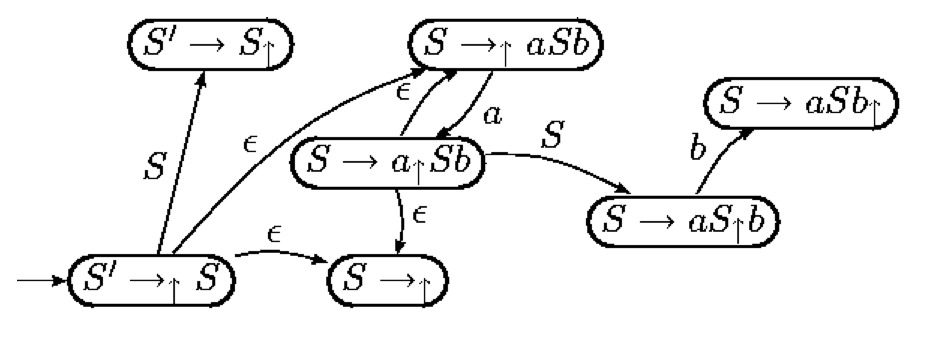
\epsfig{file=figures/nfa.eps, width=17cm}}
\caption{NFA que reconoce los prefijos viables}
\end{figure}
%\end{makeimage}
\end{center}
\end{example}

\begin{exercise}
Simule el comportamiento del autómata sobre la entrada $aabb$. ¿Donde rechaza?
¿En que estados está el autómata en el momento del rechazo?. ¿Qué etiquetas tienen?
Haga también las
trazas del autómata para las entradas $aaSbb$ y $aSb$. ¿Que antiderivación 
ha construido el autómata con sus sucesivos rechazos? ¿Que terminales
se puede esperar que hayan en la entrada cuando se produce el rechazo
del autómata?
\end{exercise}

\section{Construcción de las Tablas para el Análisis SLR}
\label{section:construcciontablasSLR}

\subsection{Los conjuntos de Primeros y Siguientes}
\label{subsection:firstandfollow}
Repasemos las nociones de conjuntos de \cei{Primeros} y \cei{siguientes}:

\begin{definition}
Dada una gramática $G=(\Sigma,V,P,S)$ y un símbolo $\alpha \in (V \cup \Sigma)^*$ se define el conjunto $FIRST(\alpha)$ como:

$FIRST(\alpha) = \left \{ b \in \Sigma :  \alpha  \stackrel{*}{\Longrightarrow}  b \beta \right \}
\cup N(\alpha)$ 

\noindent donde:

$N(\alpha) = \left \{ \begin{array}{ll}
                         \left \{ \epsilon \right \}& \mbox{si $\alpha \stackrel{*}{\Longrightarrow} \epsilon$} \\
                         \emptyset & \mbox{en otro caso} 
                      \end{array}
             \right. $ 

\end{definition}

\begin{definition}
Dada una gramática $G=(\Sigma,V,P,S)$ y una variable $A \in V$ se define el conjunto $FOLLOW(A)$ como: 

$FOLLOW(A) = \left \{ b \in \Sigma :  \exists\ S  \stackrel{*}{\Longrightarrow}  \alpha A b \beta \right \} \cup E(A)$

\noindent donde

$E(A) = \left \{ \begin{array}{ll}
                         \{ \$  \}& \mbox{si $S \stackrel{*}{\Longrightarrow} \alpha A$} \\
                         \emptyset & \mbox{en otro caso} 
                      \end{array}
             \right. $ 

\end{definition}

\begin{algorithm} Construcción de los conjuntos $FIRST(X)$
\begin{enumerate}
\item
$Si\ X \in \Sigma\ entonces\ FIRST(X) = {X}$
\item
$Si\ X \rightarrow \epsilon\ entonces\ FIRST(X) =  FIRST(X) \cup \{ \epsilon \}$
\item
$Si X \in V \ y\ X \rightarrow Y_1 Y_2 \cdots Y_k \in P\ entonces$
\begin{eqnarray*}
&&i = 1; \\
&&do\\
&&\ \ FIRST(X) = FIRST(X) \cup FIRST(Y_i) - \{ \epsilon \};\\
&&\ \ i++;\\
&&mientras\ (\epsilon \in FIRST(Y_i)\ and\ (i \leq k))\\
&&si\ (\epsilon \in FIRST(Y_k)\ and\ i > k)\ FIRST(X) = FIRST(X) \cup \{ \epsilon \}
\end{eqnarray*}
\end{enumerate}
\end{algorithm}
Este algoritmo puede ser extendido para calcular $FIRST(\alpha)$ para $\alpha = X_1 X_2 \cdots X_n \in (V \cup \Sigma)^*$.

\begin{algorithm} Construcción del conjunto $FIRST(\alpha)$ 
\begin{eqnarray*}
&&i = 1; \nonumber\\
&&FIRST(\alpha) = \emptyset; \nonumber\\
&&do \nonumber\\
&&\ \ FIRST(\alpha) = FIRST(\alpha) \cup FIRST(X_i) - \{ \epsilon \}; \nonumber\\
&&\ \ i++; \nonumber\\
&&mientras\ (\epsilon \in FIRST(X_i)\ and\ (i \leq n)) \nonumber\\
&&si\ (\epsilon \in FIRST(X_n)\ and\ i > n)\ FIRST(\alpha) = FIRST(X) \cup \{ \epsilon \}
\end{eqnarray*}
\end{algorithm} 

\begin{algorithm} Construcción de los conjuntos $FOLLOW(A)$
para las variables sintácticas $A \in V$: 

Repetir los siguientes pasos hasta que ninguno de los conjuntos $FOLLOW$ cambie:
\begin{enumerate} 
\item 
$FOLLOW(S) = \{\$\} $  ($\$$ representa el final de la entrada)
\item
$Si\ A \rightarrow \alpha B \beta\ entonces$
\[ FOLLOW(B) =  FOLLOW(B) \cup (FIRST(\beta) - \{\epsilon\})\]
\item
$Si\ A \rightarrow \alpha B$ o bien $A \rightarrow \alpha B \beta$
y $\epsilon \in FIRST(\beta)$  entonces

\[ FOLLOW(B) = FOLLOW(B) \cup FOLLOW(A)\]
\end{enumerate}
\end{algorithm}

\subsection{Construcción de las Tablas}
\label{subsection:eyappnfa2dfa}

Para la construcción de las tablas de un analizador SLR
se construye el \cei{autómata finito determinista} (\cei{DFA}) 
$(Q, \Sigma, \delta, q_0)$ equivalente al NFA 
presentado en la sección
\ref{section:eyappconceptosbasicos}
usando el \cei{algoritmo de construcción del subconjunto}.

Como recordará, en la construcción del subconjunto,
partiendo del estado de arranque $q_0$ del NFA con $\epsilon$-transiciones
se calcula su \cei{clausura} $\overline{\{q_0\}}$ y las 
clausuras de los conjuntos de estados $\overline{\delta(\overline{\{q_0\}},a)}$ 
a los que transita.  Se repite el proceso
con los conjuntos resultantes hasta que no se introducen nuevos
conjuntos-estado.

\parrafo{Clausura de un Conjunto de Estados}

La clausura $\overline{A}$ de un subconjunto de estados del autómata $A$ esta formada
por todos los estados que pueden ser alcanzados mediante transiciones
etiquetadas con la palabra vacía (denominadas $\epsilon$ transiciones)
desde los estados de $A$. Se incluyen en $\overline{A}$, naturalmente los estados 
de $A$.

\begin{center}
$\overline{A} = \{ q \in Q\ /\  \exists q' \in Q\ :\ \hat{\delta}(q, \epsilon) = q \}$
\end{center}

Aquí $\hat{\delta}$ denota la \cei{función de transición del autómata} extendida  a cadenas
de $\Sigma^*$.

\begin{equation}
\label{equation:eyappdeltahat}
\hat{\delta}(q, x) = \left \{ \begin{array}{ll}
                         \delta(\hat{\delta}(q,y),a) & \mbox{si $x = ya$} \\
                         q & \mbox{si $x = \epsilon$} 
                      \end{array}
             \right.  
\end{equation}

En la práctica, y a partir de ahora así lo haremos, se prescinde de diferenciar
entre $\delta$ y $\hat{\delta}$ usándose indistintamente la notación
$\delta$ para ambas funciones.

La clausura puede ser computada usando una estructura de pila o aplicando 
la expresión recursiva dada en la ecuación \ref{equation:eyappdeltahat}.
Una forma de computarla viene dada por el siguiente seudocódigo:
\begin{verbatim}
function closure(I : set of LR(0)-items) 
begin
  J = I;
  repeat
    changes = FALSE;
    for A->alpha . B beta in J do
      for B->gamma in G do
        next if B->.gamma in J
        insert B->.gamma in J
        changes = TRUE;
      end for
    end for
  until nochanges;
  return J
end
\end{verbatim}

\parrafo{Ejemplo de Construcción del DFA}

Para el NFA mostrado en el ejemplo \ref{example:eyappasb} el DFA construído mediante esta
técnica es el que se muestra en la figura \ref{fig:eyappdfa}. Se ha utilizado el símbolo
\verb|#| como marcador. Se ha omitido el número 3 para que los estados coincidan
en numeración con los generados por \verb|eyapp| (véase el cuadro
\ref{table:eyapptablaslalr}).

\begin{center}
\begin{figure}
\label{fig:eyappdfa}
\centerline{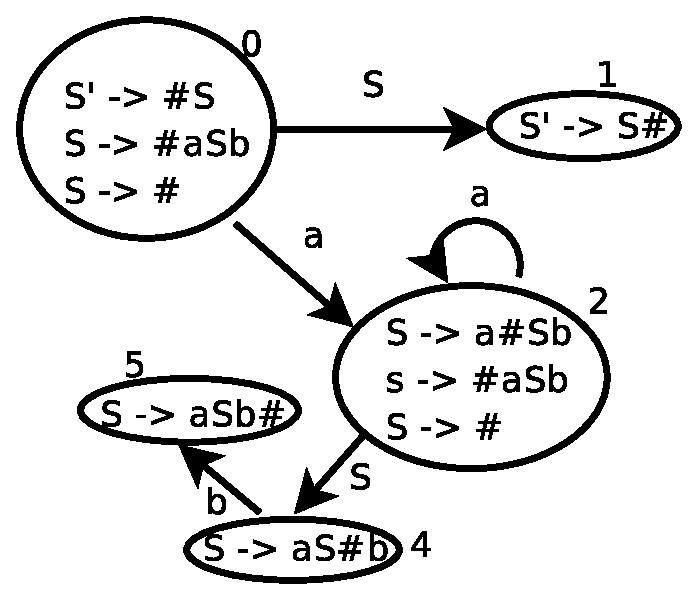
\epsfig{file=figures/dfa.eps, width=12cm}}
\caption{DFA equivalente al NFA de la figura \ref{fig:eyappnfa}}
\end{figure}
\end{center}

\parrafo{Las Tablas de Saltos y de Acciones}

Un analizador sintáctico LR utiliza una tabla para su análisis.
Esa tabla se construye a partir de la tabla de transiciones del DFA.
De hecho, la tabla se divide en dos tablas, una llamada 
\cei{tabla de saltos} o \cei{tabla de gotos} y la otra
\cei{tabla de acciones}.

La tabla \cei{goto} de un analizador \cei{SLR}
no es más que la tabla de transiciones del autómata DFA 
obtenido aplicando la construcción del subconjunto al NFA
definido en \ref{definition:eyappslrautomata}. De hecho es la tabla
de transiciones restringida a $V$ (recuerde que el alfabeto del
autómata es $V \cup \Sigma$).
Esto es, 

\begin{center}
$\delta_{| V \times Q} :  V \times Q \rightarrow Q$. 

donde se define $goto(i, A) = \delta(A,I_i)$
\end{center}

La parte de la función de transiciones
del DFA que corresponde a los terminales que no producen rechazo, 
esto es, $\delta_{| \Sigma \times Q} :  \Sigma \times Q \rightarrow Q$
se adjunta a una tabla que se denomina \cei{tabla de acciones}.
La tabla de acciones es una tabla de doble entrada en los estados
y en los símbolos de $\Sigma$.
Las acciones de transición ante terminales 
se denominan \cei{acciones de desplazamiento} o (\cei{acciones shift}):

\begin{center}
$\delta_{| \Sigma \times Q} :  \Sigma \times Q \rightarrow Q$

donde se define $action(i, a) = \delta(a,I_i)$
\end{center}

\parrafo{Ante que Terminales se debe Reducir}

Cuando un estado $s$ contiene un LR(0)-item de la forma 
$A \rightarrow \alpha_\uparrow$, 
esto es, el estado corresponde a un posible rechazo,
ello indica que hemos llegado a un final del prefijo viable, que hemos
visto $\alpha$ y que, por tanto, es probable que $A \rightarrow \alpha$
sea el \emph{handle} de la forma sentencial derecha actual. Por tanto,
añadiremos en entradas de la forma $(s,a)$ de la tabla de acciones 
una acción que indique que hemos encontrado el mango en la 
posición actual y que la regla asociada es $A \rightarrow \alpha$.
A una acción de este tipo se la denomina \cei{acción de reducción}.

La cuestión es, ¿para que valores de $a \in \Sigma$ debemos disponer que
la acción para $(s, a)$ es de reducción?
Podríamos decidir que ante cualquier terminal $a \in \Sigma$
que produzca un rechazo del autómata, pero podemos ser un poco mas
selectivos. No cualquier terminal puede estar en la entrada en el momento
en el que se produce la antiderivación o reducción. 
Observemos que si $A \rightarrow \alpha$ es el \emph{handle}
de $\gamma$ es porque:

\begin{center}
$\exists S \begin{array}{c} *\\ \Longrightarrow \\ {\scriptstyle RM} \end{array} \beta A b x \begin{array}{c} *\\ \Longrightarrow \\ {\scriptstyle RM} \end{array}  
\beta \alpha b x = \gamma$
\end{center}

Por tanto, cuando estamos reduciendo por $A \rightarrow \alpha$
los únicos terminales legales que cabe esperar en una reducción por $A \rightarrow \alpha$ son los terminales $b \in FOLLOW(A)$.

\parrafo{Algoritmo de Construcción de Las Tablas SLR}

Dada una gramática $G=(\Sigma,V,P,S)$, podemos construir las tablas de acciones (\emph{action table}) y  transiciones (\emph{gotos table}) mediante el siguiente algoritmo:

\begin{algorithm} 
\label{alg:eyapptables}       
Construcción de Tablas \cei{SLR}

\begin{enumerate}
\item
Utilizando el Algoritmo de Construcción del Subconjunto, se construye
el Autómata Finito Determinista (DFA) $(Q, V \cup \Sigma, \delta, I_0, F)$
equivalente al Autómata Finito No
Determinista (NFA) definido en \ref{definition:eyappslrautomata}.
Sea $C = \left \{ I_1, I_2, \cdots I_n \right \}$ el conjunto de estados
del DFA. Cada estado $I_i$ es un conjunto de LR(0)-items o estados
del NFA. Asociemos un índice $i$ con cada conjunto $I_i$.
\item
La tabla de \emph{gotos} no es más que la función de transición del 
autómata restringida a las variables de la gramática:

\begin{center}
$goto(i,A) = \delta(I_i, A)$ para todo $A \in V$
\end{center}
\item
Las acciones para el estado $I_i$ se determinan como sigue:
  \begin{enumerate}
  \item
  Si $A \rightarrow \alpha _\uparrow a \beta \in I_i$, $\delta(I_i,a) = I_j$, $a \in \Sigma$ 
  entonces:

\begin{center}
  $action[i][a] = shift\ j$
\end{center}
  \item
  Si $S' \rightarrow S_\uparrow \in I_i$ entonces 

\begin{center}
  $action[i][\$] = accept$
\end{center}
  \item
  Para cualquier otro caso de la forma $A \rightarrow \alpha _\uparrow \in I_i$ 
  distinto del anterior hacer

\begin{center}
  $\forall a \in\ FOLLOW(A):\ action[i][a] = reduce\ A \rightarrow \alpha$
\end{center}
  \end{enumerate}
\item
  Las entradas de la tabla de acción que queden indefinidas después de aplicado el proceso anterior corresponden a acciones de ``$error$''.
\end{enumerate}
\end{algorithm}

\parrafo{Conflictos en Un Analizador SLR}

\begin{definition}
Si alguna de las entradas de la tabla resulta multievaluada, decimos
que existe un conflicto y que la gramática no es \cei{SLR}.

\begin{enumerate}
\item
En tal caso, si una de las acciones es de `reducción'' y la otra es de
`desplazamiento'', decimos que hay un \cei{conflicto shift-reduce} o
\cei{conflicto de desplazamiento-reducción}. 
\item
Si las
dos reglas indican una acción de reducción, decimos que tenemos un 
\cei{conflicto reduce-reduce} o de \cei{reducción-reducción}.
\end{enumerate}
\end{definition}

\parrafo{Ejemplo de Cálculo de las Tablas SLR}

\begin{example}
\label{example:eyapptablasslr}
Al aplicar el algoritmo \ref{alg:eyapptables}       
a la gramática \ref{example:eyappasb} 

\vspace{0.5cm}
\begin{center}
\begin{tabular}{|l|l|}
\hline
1 & S      $\rightarrow$  a S b\\
\hline
2 & S      $\rightarrow$ $\epsilon$ \\
\hline
\end{tabular}
\end{center}
\vspace{0.25cm}

partiendo del autómata finito determinista
que se construyó en 
la figura \ref{fig:eyappdfa} y calculando los 
conjuntos de primeros y siguientes

\begin{center}
\begin{tabular}{|l|l|l|}
\hline
     & FIRST  & FOLLOW \\
\hline
S    & a, $\epsilon$ & b, \$\\
\hline
\end{tabular}
\end{center}

obtenemos la siguiente tabla de acciones SLR:

\begin{center}
\begin{tabular}{|l|l|l|l|}
\hline
     &  a  &  b  & \$ \\
\hline
0    & s2  &  r2 & r2 \\
\hline
1    &     &     & aceptar\\
\hline
2    & s2  & r2  & r2\\
\hline
4    &     & s5  &   \\
\hline
5    &     & r1  & r1\\
\hline
\end{tabular}
\end{center}

Las entradas denotadas con $s$ $n$ ($s$ por shift) indican un desplazamiento
al estado $n$, las denotadas con $r$ $n$ ($r$ por reduce o reducción) indican una operación
de reducción o antiderivación por la regla $n$.  Las entradas vacías 
corresponden a acciones de error.
\end{example}

\parrafo{Las Tablas Construidas por {\tt eyapp}}

El método de análisis \cei{LALR} usado por \verb|eyapp|
es una extensión del método SLR esbozado
aqui. Supone un compromiso entre potencia (conjunto de gramáticas
englobadas) y eficiencia (cantidad de memoria utilizada, tiempo de
proceso).
Veamos como \verb|eyapp| aplica la construcción del subconjunto a la 
gramática del ejemplo
\ref{example:eyappasb}.
Para ello construimos el siguiente programa \verb|eyapp|:
\begin{verbatim}
$ cat -n aSb.yp
     1  %%
     2  S:  # empty
     3      |   'a' S 'b'  
     4  ;
     5  %%
     ......
\end{verbatim}
y compilamos, haciendo uso de la opción \verb|-v| para que \verb|eyapp| produzca
las tablas en el fichero \verb|aSb.output|:
\begin{verbatim}
$ ls -l aSb.*
-rw-r--r--  1 lhp lhp  738 2004-12-19 09:52 aSb.output
-rw-r--r--  1 lhp lhp 1841 2004-12-19 09:52 aSb.pm
-rw-r--r--  1 lhp lhp  677 2004-12-19 09:46 aSb.yp
\end{verbatim}

El contenido del fichero \verb|aSb.output| se muestra
en la tabla 
\ref{table:eyapptablaslalr}.
Los números de referencia a las producciones en las acciones
de reducción vienen dados por:

\begin{verbatim}
                      0:	$start -> S $end
                      1:	S -> /* empty */
                      2:	S -> 'a' S 'b'
\end{verbatim} 

Observe que el final de la entrada se denota 
por \verb|$end| y el marcador en un LR-item 
por un punto. Fíjese en el estado 2: 
En ese estado están también los items

\begin{center}
 \verb|S -> . 'a' S 'b'|
y \verb|S -> .|
\end{center}

sin embargo no se explicitan
por que se entiende que su pertenencia es
consecuencia directa de aplicar la operación 
de clausura. Los LR items cuyo marcador
no está al principio se denominan
\cei{items núcleo}. 

\vspace{0.5cm}
\begin{table}[htb]
\label{table:eyapptablaslalr}
\begin{center}
\begin{tabular}{|p{4cm}|p{4cm}|p{4cm}|}
\hline
Estado 0 & Estado 1 & Estado 2\\
\hline
\begin{verbatim}
	$start -> . S $end	
	'a'	shift 2
	$default	reduce 1 (S)
	S	go to state 1
\end{verbatim} 
&
\begin{verbatim}
	$start -> S . $end	
	$end	shift 3
\end{verbatim} 
&
\begin{verbatim}
	S -> 'a' . S 'b'	
	'a'	shift 2
	$default	reduce 1 (S)
	S	go to state 4
\end{verbatim} 

\\

\hline
Estado 3 & Estado 4 & Estado 5\\
\hline

\begin{verbatim}
	$start -> S $end .	
	$default	accept
\end{verbatim} 
&
\begin{verbatim}
	S -> 'a' S . 'b'	
	'b'	shift 5
\end{verbatim} 
&
\begin{verbatim}
	S -> 'a' S 'b' .	
	$default	reduce 2 (S)
\end{verbatim}
\\
\hline
\end{tabular}
\end{center}
\caption{Tablas generadas por {\tt eyapp}. El estado 3 resulta de transitar con \$}
\end{table}
Puede encontrar el listado completo de las tablas en \verb|aSb.output|
en el apéndice que se encuentra en la página 
\ref{apendice:eyappasb}.

\begin{exercise}
Compare la tabla \ref{table:eyapptablaslalr} resultante de 
aplicar \verb|eyapp| con la que obtuvo en el ejemplo
\ref{example:eyapptablasslr}.
\end{exercise}

\section{Algoritmo de Análisis LR}
\label{section:algoritmoLR}
Asi  pues la tabla de transiciones del autómata nos genera dos tablas:
la tabla de acciones y la de saltos.
El  algoritmo  de análisis sintáctico \emph{LR} en el  que 
se basa \emph{eyapp} utiliza una pila y dos tablas 
para analizar la entrada. % (véase la figura \ref{fig:lrparser}). 
Como se ha visto, la tabla  de acciones contiene cuatro tipo de acciones: 
\begin{enumerate}
\item
Desplazar (\emph{shift})
\item
Reducir (\emph{reduce})
\item
Aceptar
\item
Error
\end{enumerate}
El algoritmo utiliza una pila en la que se guardan los estados
del autómata. De este modo se evita tener que ``comenzar'' 
el procesado de la forma sentencial derecha resultante
después de una reducción (antiderivación).
\begin{algorithm}
\label{alg:parser}       
Análizador LR
\begin{verbatim}
 my $parse = shift;
 my @stack;
 my $s0 = $parse->startstate;
 push(@stack, $s0);
 my $b = $parse->yylex();
 FOREVER: {
   my $s = top(0); 
   my $a = $b;
   switch ($parse->action[$s->state][$a]) {
     case "shift t" : 
       my $t;
       $t->{state} = t;
       $t->{attr}  = $a->{attr};
       push($t); 
       $b = $parse->yylex();
       break;
     case "reduce A ->alpha" : 
       my $r;
       $r->{attr} = $parse->Semantic{A ->alpha}->(top(|alpha|-1)->attr, ... , top(0)->attr); 
       pop(|alpha|);  # Saquemos length(alpha) elementos de la pila
       $r->{state} = $parse->goto[top(0)][A]; 
       push($r); 
       break;
     case "accept" : return ($s->attr); 
     default : $parse->yyerror("syntax error");
   }
   redo FOREVER;
 }
\end{verbatim}
\end{algorithm}
Como es habitual, $|x|$ denota la longitud de la cadena $x$.
La función \verb|top(k)| devuelve el elemento que ocupa la 
posición \verb|k| desde el \emph{top} de la pila (esto es, está a profundidad \verb|k|).
La función \verb|pop(k)| extrae \verb|k| elementos de la pila.
La notación \verb|state->attr| hace referencia al atributo
asociado con cada estado. Denotamos por \verb|$Semantic{A->alpha}|
el código de la acción asociada con la regla $A \rightarrow \alpha$.
%\begin{figure}
%\input{parser_fig.tex}
%\caption{Estructura de un Análizador LR}
%\label{fig:lrparser}       
%\end{figure}

Todos los analizadores LR comparten, salvo pequeñas
exepciones, el mismo algoritmo
de análisis. Lo que más los diferencia es la forma en 
la que construyen las tablas.
En \verb|eyapp|
la construcción de las tablas de \emph{acciones} y \emph{gotos}
se realiza mediante el algoritmo \emph{LALR}.

\begin{tabular}{|p{6.5cm}|p{6.5cm}|}
\hline
\begin{verbatim}
 1  pl@nereida:~/LEyapp/examples$ use_aSb.pl
 2  ----------------------------------------
 3  In state 0:
 4  Stack:[0]
 5  aabb
 6  Need token. Got >a<
 7  Shift and go to state 2.
 8  ----------------------------------------
 9  In state 2:
10  Stack:[0,2]
11  Need token. Got >a<
12  Shift and go to state 2.
13  ----------------------------------------
14  In state 2:
15  Stack:[0,2,2]
16  Need token. Got >b<
17  Reduce using rule 1 (S --> /* empty */): S -> epsilon
18  Back to state 2, then go to state 4.
19  ----------------------------------------
20  In state 4:
21  Stack:[0,2,2,4]
22  Shift and go to state 5.
23  ----------------------------------------
24  In state 5:
25  Stack:[0,2,2,4,5]
26  Don't need token.
27  Reduce using rule 2 (S --> a S b): S -> a S b
28  Back to state 2, then go to state 4.
29  ----------------------------------------
30  In state 4:
31  Stack:[0,2,4]
32  Need token. Got >b<
33  Shift and go to state 5.
34  ----------------------------------------
35  In state 5:
36  Stack:[0,2,4,5]
37  Don't need token.
38  Reduce using rule 2 (S --> a S b): S -> a S b
39  Back to state 0, then go to state 1.
40  ----------------------------------------
41  In state 1:
42  Stack:[0,1]
43  Need token. Got ><
44  Shift and go to state 3.
45  ----------------------------------------
46  In state 3:
47  Stack:[0,1,3]
48  Don't need token.
49  Accept.
\end{verbatim}
&
\begin{verbatim}
pl@nereida:~/LEyapp/examples$ cat -n aSb.output
 1  Rules:
 2  ------
 3  0:      $start -> S $end
 4  1:      S -> /* empty */
 5  2:      S -> 'a' S 'b'
 6
 7  States:
 8  -------
 9  State 0:
10
11          $start -> . S $end      (Rule 0)
12
13          'a'     shift, and go to state 2
14
15          $default        reduce using rule 1 (S)
16
17          S       go to state 1
18
19  State 1:
20
21          $start -> S . $end      (Rule 0)
22
23          $end    shift, and go to state 3
24
25  State 2:
26
27          S -> 'a' . S 'b'        (Rule 2)
28
29          'a'     shift, and go to state 2
30
31          $default        reduce using rule 1 (S)
32
33          S       go to state 4
34
35  State 3:
36
37          $start -> S $end .      (Rule 0)
38
39          $default        accept
40
41  State 4:
42
43          S -> 'a' S . 'b'        (Rule 2)
44
45          'b'     shift, and go to state 5
46
47  State 5:
48
49          S -> 'a' S 'b' .        (Rule 2)
50
51          $default        reduce using rule 2 (S)
52
53
54  Summary:
55  --------
56  Number of rules         : 3
57  Number of terminals     : 3
58  Number of non-terminals : 2
59  Number of states        : 6
\end{verbatim}\\
\hline
\end{tabular}
\section{Precedencia y Asociatividad}
\label{section:prioridades}
Recordemos que si al construir la tabla LALR,
alguna de las entradas de la tabla resulta multievaluada, decimos
que existe un conflicto.
Si una de las acciones es de `reducción'' y la otra es de
`desplazamiento'', se dice que hay un \cei{conflicto shift-reduce} o
\cei{conflicto de desplazamiento-reducción}. Si las
dos reglas indican una acción de reducción, decimos que tenemos un 
\cei{conflicto reduce-reduce} o de \cei{reducción-reducción}.
En caso de que no existan indicaciones específicas \emph{eyapp} resuelve
los conflictos que aparecen en la construcción de la tabla utilizando
las siguientes reglas:

\begin{enumerate}
\item
Un conflicto \emph{reduce-reduce} se resuelve eligiendo la producción
que se listó primero en la especificación de la gramática.
\item
Un conflicto \emph{shift-reduce} se resuelve siempre en favor del \emph{shift}
\end{enumerate}

Las declaraciones de precedencia y asociatividad mediante las
palabras reservadas \tei{\%left}, \tei{\%right}, \tei{\%nonassoc}
se utilizan para modificar estos criterios por defecto. 
La declaración de \tei{token}s mediante la palabra
reservada \tei{\%token} no modifica la precedencia. Si lo hacen las
declaraciones realizadas usando las palabras \tei{left}, \tei{right}
y \tei{nonassoc}. 

\begin{enumerate}
\item
Los \emph{tokens} declarados  en la misma línea
tienen igual precedencia e igual asociatividad. 
La precedencia es mayor cuanto mas abajo 
su posición en
el texto. Así, en el ejemplo de la calculadora en la sección 
\ref{section:ejemplodeuso}, el \emph{token} \verb1*1 tiene 
mayor precedencia que \verb1+1 pero la misma que \verb1/1.
\item
La precedencia de una regla $A \rightarrow \alpha$ se
define como la del terminal mas a la derecha que aparece en
$\alpha$. En el ejemplo, la producción 

\begin{center}
\verb1 expr : expr '+' expr1 
\end{center}

tiene la precedencia del \emph{token} \verb1+1.
\item
Para decidir en un conflicto \emph{shift-reduce} se comparan la precedencia 
de la regla con la del terminal que va a ser desplazado. Si la de la
regla es mayor se reduce
si la del \emph{token} es mayor, se desplaza.
\item
Si en un conflicto \emph{shift-reduce} ambos la regla y el terminal que
va a ser desplazado tiene la misma precedencia \emph{eyapp} considera la
asociatividad, si es asociativa a izquierdas, reduce y si es asociativa
a derechas desplaza. Si no es asociativa, genera un mensaje de error.\\
Obsérvese que, en esta situación, la asociatividad de la regla y la del
\emph{token} han de ser por fuerza, las mismas.  Ello es así, porque en
\emph{eyapp} los \emph{tokens} con la misma precedencia se declaran en
la misma línea y sólo se permite una declaración por línea.

\item
\emph{ Por tanto es imposible declarar dos \emph{tokens} con diferente
asociatividad y la misma precedencia}.
\item
Es posible modificar la precedencia ``natural'' de una regla, calificándola
con un \emph{token} específico.  para ello se escribe a la derecha de
la regla \verb|prec token|, donde \verb|token| es un \emph{token} con
la precedencia que deseamos. Vea el uso del \emph{token} \verb|dummy|
en el siguiente ejercicio.
\end{enumerate}


Para ilustrar las reglas anteriores usaremos el siguiente 
programa \verb|eyapp|:

\begin{verbatim}
$ cat -n Precedencia.yp
     1  %token NUMBER
     2  %left '@'
     3  %right '&'  dummy
     4  %%
     5  list
     6      :
     7      | list '\n'
     8      | list e
     9      ;
    10
    11  e : NUMBER
    12    | e '&' e
    13    | e '@' e %prec dummy
    14    ;
    15
    16  %%
\end{verbatim}            

El código del programa cliente es el siguiente:

\begin{verbatim}
$ cat -n useprecedencia.pl
cat -n useprecedencia.pl
     1  #!/usr/bin/perl -w
     2  use strict;
     3  use Precedencia;
     4
     5  sub Error {
     6    exists $_[0]->YYData->{ERRMSG}
     7    and do {
     8      print $_[0]->YYData->{ERRMSG};
     9      delete $_[0]->YYData->{ERRMSG};
    10      return;
    11    };
    12    print "Syntax error.\n";
    13  }
    14
    15  sub Lexer {
    16    my($parser)=shift;
    17
    18    defined($parser->YYData->{INPUT})
    19    or  $parser->YYData->{INPUT} = <STDIN>
    20    or  return('',undef);
    21
    22    $parser->YYData->{INPUT}=~s/^[ \t]//;
    23
    24    for ($parser->YYData->{INPUT}) {
    25        s/^([0-9]+(?:\.[0-9]+)?)//
    26                and return('NUMBER',$1);
    27        s/^(.)//s
    28                and return($1,$1);
    29    }
    30  }
    31
    32  my $debug_level = (@ARGV)? oct(shift @ARGV): 0x1F;
    33  my $parser = Precedencia->new();
    34  $parser->YYParse( yylex => \&Lexer, yyerror => \&Error, yydebug => $debug_level );
\end{verbatim}

Observe la llamada al analizador en la línea 34. Hemos 
añadido el parámetro con nombre \cei{yydebug} 
con argumento \verb|yydebug => $debug_level| (véase la
sección \ref{section:depuracion} para ver los posibles
valores de depuración).

Compilamos a continuación el módulo usando la opción \verb|-v| para
producir información sobre los conflictos y las tablas de salto y 
de acciones:
\begin{verbatim}
eyapp -v -m Precedencia Precedencia.yp
$ ls -ltr |tail -2
-rw-r--r--  1 lhp lhp   1628 2004-12-07 13:21 Precedencia.pm
-rw-r--r--  1 lhp lhp   1785 2004-12-07 13:21 Precedencia.output
\end{verbatim}

La opción \verb|-v| genera el fichero \verb|Precedencia.output|
el cual contiene información detallada sobre el autómata:

\begin{verbatim}
$ cat -n Precedencia.output
     1  Conflicts:
     2  ----------
     3  Conflict in state 8 between rule 6 and token '@' resolved as reduce.
     4  Conflict in state 8 between rule 6 and token '&' resolved as shift.
     5  Conflict in state 9 between rule 5 and token '@' resolved as reduce.
     6  Conflict in state 9 between rule 5 and token '&' resolved as shift.
     7
     8  Rules:
     9  ------
    10  0:      $start -> list $end
    11  1:      list -> /* empty */
    12  2:      list -> list '\n'
    13  3:      list -> list e
    14  4:      e -> NUMBER
    15  5:      e -> e '&' e
    16  6:      e -> e '@' e
    17  ...
\end{verbatim}
¿Porqué se produce un conflicto en el estado 8 entre la regla
6 (\verb|e -> e '@' e|) y el terminal \verb|'@'|?. Editando el fichero
\verb|Precedencia.output| podemos ver los contenidos
del estado 8:
\begin{verbatim}
85  State 8:
86
87          e -> e . '&' e  (Rule 5)
88          e -> e . '@' e  (Rule 6)
89          e -> e '@' e .  (Rule 6)
90
91          '&'     shift, and go to state 7
92
93          $default        reduce using rule 6 (e)
\end{verbatim}
El item de la línea 88 indica que debemos desplazar, el de 
la línea 89 que debemos reducir por la regla 6. ¿Porqué \verb|eyapp|
resuelve el conflicto optando por reducir?
¿Que prioridad tiene la regla 6?
¿Que asociatividad tiene la regla 6?
La declaración en la línea 13 modifica la precedencia y asociatividad
de la regla:

\begin{verbatim}
    13    | e '@' e %prec dummy
\end{verbatim}

de manera que la regla pasa a tener la precedencia y asociatividad
de \verb|dummy|. Recuerde que habíamos declarado \verb|dummy| como
asociativo a derechas:
\begin{verbatim}
     2  %left '@'
     3  %right '&'  dummy
\end{verbatim}
¿Que ocurre? Que \verb|dummy| tiene mayor prioridad
que \verb|'@'| y por tanto la regla tiene mayor prioridad
que el terminal: por tanto se reduce.

¿Que ocurre cuando el terminal en conflicto es \verb|'&'|?
En ese caso la regla y el terminal tienen la misma prioridad.
Se hace uso de la asociatividad a derechas que indica que el conflicto
debe resolverse desplazando.

\begin{exercise}
Explique la forma en que \verb|eyapp| resuelve 
los conflictos que aparecen en el estado 9.
Esta es la información sobre el estado 9:

\begin{verbatim}
State 9:

	e -> e . '&' e	(Rule 5)
	e -> e '&' e .	(Rule 5)
	e -> e . '@' e	(Rule 6)
	'&'	shift, and go to state 7
	$default	reduce using rule 5 (e)
\end{verbatim}
\end{exercise}

Veamos un ejemplo de ejecución:

\begin{verbatim}
$ ./useprecedencia.pl
----------------------------------------
In state 0:
Stack:[0]
Don't need token.
Reduce using rule 1 (list,0): Back to state 0, then go to state 1.
\end{verbatim}
Lo primero que ocurre es una reducción por la regla 
en la que \verb|list| produce vacío. Si miramos el estado 0
del autómata vemos que contiene:
\begin{verbatim}
20 State 0:
21
22   $start -> . list $end (Rule 0)
23
24   $default  reduce using rule 1 (list)
25
26   list  go to state 1
\end{verbatim}
A continuación se transita desde 0 con \verb|list|
y se consume el primer terminal:
\begin{verbatim}
----------------------------------------
In state 1:
Stack:[0,1]
2@3@4
Need token. Got >NUMBER<
Shift and go to state 5.
----------------------------------------
In state 5:
Stack:[0,1,5]
Don't need token.
Reduce using rule 4 (e,1): Back to state 1, then go to state 2.
----------------------------------------
\end{verbatim}
En el estado 5 se reduce por la regla \verb|e -> NUMBER|.
Esto hace que se retire el estado 5 de la pila y se
transite desde el estado 1 viendo el símbolo \verb|e|:
\begin{verbatim}
In state 2:
Stack:[0,1,2]
Need token. Got >@<
Shift and go to state 6.
----------------------------------------
In state 6:
Stack:[0,1,2,6]
Need token. Got >NUMBER<
Shift and go to state 5.
----------------------------------------
In state 5:
Stack:[0,1,2,6,5]
Don't need token.
Reduce using rule 4 (e,1): Back to state 6, then go to state 8.
----------------------------------------
In state 8:
Stack:[0,1,2,6,8]
Need token. Got >@<
Reduce using rule 6 (e,3): Back to state 1, then go to state 2.
----------------------------------------
...
Accept.
\end{verbatim}
Obsérvese la resolución del conflicto en el estado 8

La presencia de conflictos, aunque no siempre, en muchos casos es debida
a la introducción de ambiguedad en la gramática. Si el conflicto 
es de desplazamiento-reducción se puede resolver explicitando 
alguna regla que rompa la ambiguedad. Los conflictos de
reducción-reducción suelen producirse por un diseño erróneo
de la gramática. En tales casos, suele ser mas adecuado
modificar la gramática.

\section{Acciones en Medio de una Regla}
\label{section:mediaregla}
A veces necesitamos insertar una acción en medio de una regla.
Una acción en medio de una regla puede hacer referencia a los atributos de
los símbolos que la preceden (usando \verb|$n|), pero no a los que le siguen.

Cuando se  inserta una acción $\left \{ action_1\right \}$
para su ejecución en medio de una regla $A \rightarrow \alpha
\beta$ :
\begin{center}
$A \rightarrow \alpha \left \{ action_1 \right \} \beta \left \{ action_2\right \}$ 
\end{center}
\verb|eyapp| crea una variable sintáctica temporal $T$ e introduce una nueva regla:

\begin{center}
\begin{enumerate}
\item
$A \rightarrow \alpha T \beta \left \{ action_2\right \}$ 
\item
$T \rightarrow \epsilon \left \{ action_1 \right \}$ 
\end{enumerate}
\end{center}

Las acciones en mitad de una regla cuentan como un símbolo mas en la parte 
derecha de la regla. Asi pues, en una acción posterior en la regla,
se deberán referenciar los  atributos de los símbolos, teniendo en cuenta este hecho.

Las acciones en mitad de la regla pueden tener un atributo. 
Las acciones posteriores
en la regla se referirán a él como \verb|$_[n]|, siendo \verb|n| su número de orden
en la parte derecha. 

Observe que la existencia de acciones intermedias 
implica que la gramática inicial es modificada. La introducción  de las nuevas 
reglas puede dar lugar a ambiguedades y/o conflictos. Es responsabilidad
del programador eliminarlos.
Por ejemplo, dada la gramática:
\begin{verbatim}
cs : '{' decs ss '}' | '{' ss '}' ;
\end{verbatim}
Si la modificamos como sigue:
\begin{verbatim}
cs : { decl(); } '{' decs ss '}' 
   | '{' ss '}' 
   ;
\end{verbatim}
habremos introducido un conflicto.

\begin{exercise}
Explique las razones por las cuales la introducción de la acción que prefija
la primera regla da lugar a conflictos
\end{exercise}

\begin{exercise}
El conflicto no se arregla haciendo 
que la acción que precede sea la misma:
\begin{verbatim}
cs : { decl(); } '{' decs ss '}' 
   | { decl(); } '{' ss '}' 
   ;
\end{verbatim}
Explique donde está el fallo de esta propuesta
\end{exercise}

\begin{exercise}
¿Se arregla el conflicto anterior usando esta otra alternativa?

\begin{verbatim}
cs :  tp '{' decs ss '}' 
   |  tp { decl(); } '{' ss '}' 
   ;
   
tp : /* empty */ { decl(); }
   ;
\end{verbatim}
\end{exercise}

\section{Manejo en {\tt eyapp} de Atributos Heredados}
\label{section:heredados}
Supongamos  que \verb|eyapp| esta inmerso 
en la construcción de la antiderivación a derechas y que la forma sentencial
derecha en ese momento es:

\begin{center}
$X_m \ldots X_1 X_0 Y_1 \ldots  Y_n a_1 \ldots a_0$
\end{center}

y que el mango es $B \rightarrow Y_1 \ldots  Y_n$ y en la entrada quedan por 
procesar $a_1 \ldots a_0$.

Es posible acceder en \verb|eyapp| a los valores de los atributos de los estados en la pila
del analizador que se encuentran ``por debajo'' o si se quiere
``a la izquierda'' de los estados asociados
con la regla por la que se reduce. Para ello se usa una llamada al método
\cei{{\tt YYSemval}}. La llamada es de la forma 
\verb|$_[0]->YYSemval( index )|, donde \verb|index| es un entero.
Cuando se usan los valores \verb|1| \ldots \verb|n| devuelve lo mismo
que \verb|$_[1]|, \ldots \verb|$_[n]|. Esto es 
\verb|$_[1]| es el atributo asociado con $Y_1$ y \verb|$_[n]| es el atributo
asociado con $Y_n$.  Cuando se usa con el valor
0 devolverá el valor del atributo asociado con el símbolo que esta a la izquierda 
del mango actual, esto es el atributo asociado con $X_0$, 
si se llama con -1 el que está dos unidades a la izquierda de la variable actual, 
esto es, el asociado con $X_1$ etc. Así \verb|$_[-m]| denota el atributo
de $X_m$.

Esta forma de acceder a los atributos es especialmente útil cuando se 
trabaja con \cei{atributos heredados}. Esto es, cuando un atributo
de un nodo del árbol sintáctico se computa en términos
de valores de atributos de su padre y/o sus hermanos.
Ejemplos de atributos heredados son la clase y tipo en la declaración
de variables. Supongamos que tenemos el siguiente 
\cei{esquema de traducción} para calcular la clase (C) y tipo (T) en 
las declaraciones (D) de listas (L) de identificadores:

\vspace{0.5cm}
\begin{center}
\begin{tabular}{|l|ll|}
\hline
1 & D $\rightarrow$& C T \verb|{ $L{c} = $C{c}; $L{t} = $T{t} }| L\\
2 & C $\rightarrow$& global   \verb|{ $C{c} = "global" }|\\
3 & C $\rightarrow$& local    \verb|{ $C{c} = "local" }|\\
4 & T $\rightarrow$& integer  \verb|{ $T{t} = "integer" }|\\
5 & T $\rightarrow$& float    \verb|{ $T{t} = "float" }|\\
6 & L $\rightarrow$& \verb|{ $L|$_1$\verb|{t} = $L{t}; $L|$_1$\verb|{c} = $L{c}; }| L$_1$ ','\\
7 &                & id \verb|{ set_class($id{v}, $L{c}); set_type($id{v}, $L{t}); }|\\
8 & L $\rightarrow$& id   \verb|{ set_class($id{v}, $L{c}); set_type($id{v}, $L{t}); }|\\
\hline
\end{tabular}
\end{center}
\vspace{0.25cm}

Los atributos \verb|c| y \verb|t| denotan respectivamente
la clase y el tipo. 

\begin{exercise}
Evalúe el esquema de traducción para la entrada
\verb|global float x,y|. Represente el árbol de análisis, las
acciones incrustadas y determine el orden de ejecución.

Olvide por un momento la notación usada en las acciones y 
suponga que se tratara de acciones \verb|eyapp|. ¿En que orden
construye \verb|eyapp| el árbol y en que orden ejecutará las
acciones?
\end{exercise}

Observe que la simple razón por la cual la acción intermedia
\verb|{ $L|$_1$\verb|{t} = $L{t}; $L|$_1$\verb|{c} = $L{c}; }|
no puede ser ejecutada en un programa \verb|eyapp| es porque 
el nodo
del árbol sintáctico asociado con {\tt L}$_1$ no existe
en el momento en el que la acción es ejecutada. No es posible
guardar algo en {\tt L}$_1$\verb|{c}| ya que no hay nodo asociado
con {\tt L}$_1$. 
La situación es 
distinta si se esta trabajando con un esquema de traducción
ya que estos primero construyen el árbol y luego lo recorren.

A la hora de transformar este esquema de traducción en un programa
\verb|eyapp| es importante darse cuenta que en cualquier derivación a derechas
desde D, cuando se reduce por una de las reglas 

\begin{center}
L $\rightarrow$ id $|$ L$_1$  ',' id
\end{center}

el símbolo a la izquierda de L es T y el que esta a la izquierda de T es C.
Considere, por ejemplo la derivación a derechas:

\begin{center}
D $\Longrightarrow$ C T L $\Longrightarrow$ C T L, id $\Longrightarrow$ C T L, id, id
$\Longrightarrow$ C T id, id, id $\Longrightarrow$ \\
$\Longrightarrow$ C float id, id, id $\Longrightarrow$ local float id, id, id
\end{center}

\noindent Observe que el orden de recorrido de \verb|eyapp| es:
\begin{center}
local float id, id, id $\Longleftarrow$ C float id, id $\Longleftarrow$
C T id, id, id $\Longleftarrow$\\
$\Longleftarrow$ C T L, id, id $\Longleftarrow$ C T L, id $\Longleftarrow$ C T L $\Longleftarrow$ D
\end{center}

\noindent en la antiderivación, cuando el mango es una de las dos reglas 
para listas de identificadores, L $\rightarrow$ id y L $\rightarrow$ L, id 
es decir durante las tres ultimas antiderivaciones:

\begin{center}
C T L, id, id $\Longleftarrow$ C T L, id $\Longleftarrow$ C T L $\Longleftarrow$ D
\end{center}

\noindent las variables a la izquierda del mango son
T y C. Esto ocurre siempre. 
Estas observaciones nos conducen al siguiente
programa \verb|eyapp|: 

\begin{verbatim}
$ cat -n Inherited.yp
 1  %token FLOAT INTEGER
 2  %token GLOBAL
 3  %token LOCAL
 4  %token NAME
 5
 6  %%
 7  declarationlist
 8    : # vacio
 9    | declaration ';' declarationlist
10    ;
11
12  declaration
13    : class type namelist { ; }
14    ;
15
16  class
17    : GLOBAL
18    | LOCAL
19    ;
20
21  type
22    : FLOAT
23    | INTEGER
24    ;
25
26  namelist
27    : NAME
28       { printf("%s de clase %s, tipo %s\n",
29               $_[1], $_[0]->YYSemval(-1),$_[0]->YYSemval(0)); }
30    | namelist ',' NAME
31        { printf("%s de clase %s, tipo %s\n",
32                 $_[3], $_[0]->YYSemval(-1),$_[0]->YYSemval(0)); }
33    ;
34  %%
\end{verbatim}

A continuación escribimos el programa que usa 
el módulo generado por \verb|eyapp|:

\begin{verbatim}
$ cat -n useinherited.pl
 1  #!/usr/bin/perl -w
 2  use strict;
 3  use Inherited;
 4
 5  sub Error {
 6    exists $_[0]->YYData->{ERRMSG}
 7    and do {
 8      print $_[0]->YYData->{ERRMSG};
 9      delete $_[0]->YYData->{ERRMSG};
10      return;
11    };
12    print "Error sintáctico\n";
13  }
14
15  { # hagamos una clausura con la entrada
16    my $input;
17    local $/ = undef;
18    print "Entrada (En Unix, presione CTRL-D para terminar):\n";
19    $input = <stdin>;
20
21    sub scanner {
22
23      { # Con el redo del final hacemos un bucle "infinito"
24        if ($input =~ m|\G\s*INTEGER\b|igc) {
25          return ('INTEGER', 'INTEGER');
26        }
27        elsif ($input =~ m|\G\s*FLOAT\b|igc) {
28          return ('FLOAT', 'FLOAT');
29        }
30        elsif ($input =~ m|\G\s*LOCAL\b|igc) {
31          return ('LOCAL', 'LOCAL');
32        }
33        elsif ($input =~ m|\G\s*GLOBAL\b|igc) {
34          return ('GLOBAL', 'GLOBAL');
35        }
36        elsif ($input =~ m|\G\s*([a-z_]\w*)\b|igc) {
37          return ('NAME', $1);
38        }
39        elsif ($input =~ m/\G\s*([,;])/gc) {
40          return ($1, $1);
41        }
42        elsif ($input =~ m/\G\s*(.)/gc) {
43          die "Caracter invalido: $1\n";
44        }
45        else {
46          return ('', undef); # end of file
47        }
48        redo;
49      }
50    }
51  }
52
53  my $debug_level = (@ARGV)? oct(shift @ARGV): 0x1F;
54  my $parser = Inherited->new();
55  $parser->YYParse( yylex => \&scanner, yyerror => \&Error, yydebug => $debug_level );
\end{verbatim}
En las líneas de la 15 a la 51 esta nuestro analizador léxico.
La entrada se lee en una variable local cuyo valor permanece
entre llamadas: hemos creado una clausura con la variable
\verb|$input| (véase la sección \eref{section:clausura} para mas detalles
sobre el uso de clausuras en Perl). Aunque la variable \verb|$input|
queda inaccesible desde fuera de la clausura, persiste entre llamadas
como consecuencia de que la subrutina \verb|scanner| la utiliza.

A continuación sigue un ejemplo de ejecución:

\begin{verbatim}
$ ./useinherited.pl 0
Entrada (En Unix, presione CTRL-D para terminar):
global integer x, y, z;
local float a,b;
x de clase GLOBAL, tipo INTEGER
y de clase GLOBAL, tipo INTEGER
z de clase GLOBAL, tipo INTEGER
a de clase LOCAL, tipo FLOAT
b de clase LOCAL, tipo FLOAT
\end{verbatim}

%\begin{exercise}
%El siguiente programa \verb|eyapp| calcula 
%un árbol de análisis abstracto para la gramática
%del ejemplo anterior:
%\begin{verbatim}
%%token FLOAT INTEGER 
%%token GLOBAL 
%%token LOCAL 
%%token NAME
%
%%%
%declarationlist 
%  : /* vacio */                     { bless [], 'declarationlist' } 
%  | declaration ';' declarationlist { push @{$_[3]}, $_[1]; $_[3] }
%  ;
%
%declaration
%  : class type namelist 
%      { 
%        bless {class => $_[1], type => $_[2], namelist => $_[3]}, 'declaration'; 
%      }
%  ;
%
%class
%  : GLOBAL  { bless { GLOBAL => 0}, 'class' } 
%  | LOCAL   { bless { LOCAL => 1}, 'class' }
%  ;
%
%type
%  : FLOAT   { bless { FLOAT => 2}, 'type' } 
%  | INTEGER { bless { INTEGER => 3}, 'type' }
%  ;
%
%namelist
%  : NAME  
%     { bless [ $_[1]], 'namelist' }
%  | namelist ',' NAME 
%      { push @{$_[1]}, $_[3]; $_[1] }
%  ;
%%%
%\end{verbatim}
%sigue un ejemplo de ejecución:
%\begin{verbatim}
%$ ./useinherited3.pl
%Entrada (En Unix, presione CTRL-D para terminar):
%global float x,y;
%$VAR1 = bless( [
%  bless( {
%    'namelist' => bless( [ 'x', 'y' ], 'namelist' ),
%    'type' => bless( { 'FLOAT' => 2 }, 'type' ),
%    'class' => bless( { 'GLOBAL' => 0 }, 'class' )
%  }, 'declaration' )
%], 'declarationlist' );
%\end{verbatim}
%
%Extienda el programa del ejemplo para que la gramática 
%incluya las acciones del esquema de traducción.
%Las acciones se tratarán como un terminal \verb|CODE|
%y serán devueltas por el analizador léxico. Su atributo
%asociado es el texto del código. El programa 
%\verb|eyapp| deberá devolver el árbol abstracto
%extendido con las acciones-terminales.
%La parte mas difícil de este problema consiste en ``reconocer''
%el código Perl incrustado. La estrategia seguir consiste
%en contar el número de llaves que se abren y se cierran.
%Cuando el contador alcanza cero es que hemos llegado
%al final del código Perl incrustado. Esta estrategia
%tiene una serie de problemas. ¿Sabría decir cuáles?
%(sugerencia: repase la sección \ref{subsection:elcuerpo} 
%o vea como \verb|eyapp| resuelve el problema).
%\end{exercise}

\section{Acciones en Medio de una Regla y Atributos Heredados}
\label{section:mediaregla}
La estrategia utilizada en la sección \ref{section:heredados} funciona
si podemos predecir la posición del atributo en la pila del analizador.
En el ejemplo anterior los atributos clase y tipo estaban siempre,
cualquiera que fuera la derivación a derechas, 
en las posiciones 0 y -1. Esto no siempre es asi. Consideremos
la siguiente \cei{definición dirigida por la sintáxis}:

\vspace{0.5cm}
\begin{center}
\begin{tabular}{|l|l|}
\hline
S $\rightarrow$ a A C   & \verb|$C{i} = $A{s}|\\
\hline
S $\rightarrow$ b A B C & \verb|$C{i} = $A{s}|\\
\hline
C $\rightarrow$ c       & \verb|$C{s} = $C{i}|\\
\hline
A $\rightarrow$ a       & \verb|$A{s} = "a"|\\
\hline
B $\rightarrow$ b       & \verb|$B{s} = "b"|\\
\hline
\end{tabular}
\end{center}
\vspace{0.25cm}


\begin{exercise}
Determine un orden correcto de evaluación de la anterior
definición dirigida por la sintáxis para la entrada \verb|b a b c|.
\end{exercise}

C hereda el atributo sintetizado de A. El problema es que, en la pila
del analizador el atributo \verb|$A{s}| puede estar en la posición 0 
o -1 dependiendo de si la regla por la que se derivó fué
S $\rightarrow$ a A C o bien S $\rightarrow$ b A B C. La solución
a este tipo de problemas consiste en insertar acciones 
intermedias de copia del atributo de manera que se garantize que el atributo
de interés está siempre a una distancia fija. Esto es, se inserta
una variable sintáctica intermedia auxiliar M la cual deriva a vacío
y que tiene como acción asociada una regla de copia:

\vspace{0.5cm}
\begin{center}
\begin{tabular}{|l|l|}
\hline
S $\rightarrow$ a A C   & \verb|$C{i} = $A{s}|\\
\hline
S $\rightarrow$ b A B M C & \verb|$M{i} = $A{s}; $C{i} = $M{s}|\\
\hline
C $\rightarrow$ c       & \verb|$C{s} = $C{i}|\\
\hline
A $\rightarrow$ a       & \verb|$A{s} = "a"|\\
\hline
B $\rightarrow$ b       & \verb|$B{s} = "b"|\\
\hline
M $\rightarrow \epsilon$& \verb|$M{s} = $M{i}|\\
\hline
\end{tabular}
\end{center}
\vspace{0.25cm}

El nuevo esquema de traducción puede ser implantado mediante
un programa \verb|eyapp|:

\begin{verbatim}
$ cat -n Inherited2.yp
     1  %%
     2  S : 'a' A C
     3    | 'b' A B  { $_[2]; } C
     4    ;
     5
     6  C : 'c' { print "Valor: ",$_[0]->YYSemval(0),"\n"; $_[0]->YYSemval(0) }
     7    ;
     8
     9  A : 'a' { 'a' }
    10    ;
    11
    12  B : 'b' { 'b' }
    13    ;
    14
    15  %%
\end{verbatim}

La ejecución muestra como se ha propagado el valor del atributo:
\begin{verbatim}
$ ./useinherited2.pl '0x04'
Entrada (En Unix, presione CTRL-D para terminar):
b a b c
Shift 2.  Shift 6.
Reduce using rule 5 (A,1): Back to state 2, then state 5.
Shift 8.
Reduce 6 (B,1): Back to state 5, then state 9.
Reduce 2 (@1-3,0): Back to state 9, then state 12.
\end{verbatim}

En este momento se esta ejecutando la acción intermedia.
Lo podemos comprobar revisando el fichero \verb|Inherited2.output|
que fué generado usando la opción \verb|-v| al llamar a \verb|eyapp|.
La regla 2 por la que se reduce es la asociada con la acción 
intermedia:

\begin{verbatim}
$ cat -n Inherited2.output
     1  Rules:
     2  ------
     3  0:      $start -> S $end
     4  1:      S -> 'a' A C
     5  2:      @1-3 -> /* empty */
     6  3:      S -> 'b' A B @1-3 C
     7  4:      C -> 'c'
     8  5:      A -> 'a'
     9  6:      B -> 'b'
        ...
\end{verbatim}

Obsérvese la notación usada por \verb|eyapp| para la 
\cei{acción en medio de la regla}: \verb|@1-3|.
Continuamos con la antiderivación:

\begin{verbatim}
Shift 10.
Reduce 4 (C,1): 
Valor: a
Back to state 12, then 13.
Reduce using rule 3 (S,5): Back to state 0, then state 1.
Shift 4.
Accept.
\end{verbatim}

El método puede ser generalizado a casos en los
que el atributo de interés este a diferentes distancias en
diferentes reglas sin mas que introducir las correspondientes
acciones intermedias de copia.

